% A LaTeX (non-official) template for ISAE projects reports
% Copyright (C) 2014 Damien Roque
% Version: 0.2
% Author: Damien Roque <damien.roque_AT_isae.fr>

\documentclass[oneside]{book}
\usepackage[utf8]{inputenc}
\usepackage[T1]{fontenc}
\usepackage[frenchb]{babel} % If you write in French
%\usepackage[english]{babel} % If you write in English
\usepackage{a4wide}
\usepackage{graphicx}
\graphicspath{{images/}}
\usepackage{subfig}
\usepackage{tikz}
\usetikzlibrary{shapes,arrows}
\usepackage{pgfplots}
\pgfplotsset{compat=newest}
\pgfplotsset{plot coordinates/math parser=false}
\newlength\figureheight
\newlength\figurewidth
\pgfkeys{/pgf/number format/.cd,
set decimal separator={,\!},
1000 sep={\,},
}
\usepackage{ifthen}
\usepackage{ifpdf}
\usepackage{afterpage}
\ifpdf
\usepackage[pdftex]{hyperref}
\else
\usepackage{hyperref}
\fi
\usepackage{color}
\hypersetup{%
colorlinks=true,
linkcolor=black,
citecolor=black,
urlcolor=black}

\usepackage{lipsum}
\usepackage{titlesec}
\usepackage{sectsty}
\usepackage{eurosym}
\usepackage{listings}  




\usepackage{etoolbox}% http://ctan.org/pkg/etoolbox


\renewcommand{\contentsname}{test}

\renewcommand{\baselinestretch}{1.05}
\usepackage{fancyhdr}
\pagestyle{fancy}
\fancyfoot{}
\fancyhead[LO]{\bfseries\nouppercase{\rightmark}}
\setlength{\headheight}{15pt}

\let\headruleORIG\headrule
\renewcommand{\headrule}{\color{black} \headruleORIG}
\renewcommand{\headrulewidth}{1.0pt}
\usepackage{colortbl}
\arrayrulecolor{black}

\fancypagestyle{plain}{
  \fancyhead{}
  \fancyfoot[C]{\thepage}
  \renewcommand{\headrulewidth}{0pt}
}

\makeatletter
\def\@textbottom{\vskip \z@ \@plus 1pt}
\let\@texttop\relax
\makeatother

\makeatletter
\def\cleardoublepage{\clearpage\if@twoside \ifodd\c@page\else%
  \hbox{}%
  \thispagestyle{empty}%
  \newpage%
  \if@twocolumn\hbox{}\newpage\fi\fi\fi}
\makeatother

\usepackage{amsthm}
\usepackage{amssymb,amsmath,bbm}
\usepackage{array}
\usepackage{bm}
\usepackage{multirow}
\usepackage[footnote]{acronym}

\newcommand*{\SET}[1]  {\ensuremath{\mathbf{#1}}}
\newcommand*{\VEC}[1]  {\ensuremath{\boldsymbol{#1}}}
\newcommand*{\FAM}[1]  {\ensuremath{\boldsymbol{#1}}}
\newcommand*{\MAT}[1]  {\ensuremath{\boldsymbol{#1}}}
\newcommand*{\OP}[1]  {\ensuremath{\mathrm{#1}}}
\newcommand*{\NORM}[1]  {\ensuremath{\left\|#1\right\|}}
\newcommand*{\DPR}[2]  {\ensuremath{\left \langle #1,#2 \right \rangle}}
\newcommand*{\calbf}[1]  {\ensuremath{\boldsymbol{\mathcal{#1}}}}
\newcommand*{\shift}[1]  {\ensuremath{\boldsymbol{#1}}}

\newcommand{\eqdef}{\stackrel{\mathrm{def}}{=}}
\newcommand{\argmax}{\operatornamewithlimits{argmax}}
\newcommand{\argmin}{\operatornamewithlimits{argmin}}
\newcommand{\ud}{\, \mathrm{d}}
\newcommand{\vect}{\text{Vect}}
\newcommand{\sinc}{\ensuremath{\mathrm{sinc}}}
\newcommand{\esp}{\ensuremath{\mathbb{E}}}
\newcommand{\hilbert}{\ensuremath{\mathcal{H}}}
\newcommand{\fourier}{\ensuremath{\mathcal{F}}}
\newcommand{\sgn}{\text{sgn}}
\newcommand{\intTT}{\int_{-T}^{T}}
\newcommand{\intT}{\int_{-\frac{T}{2}}^{\frac{T}{2}}}
\newcommand{\intinf}{\int_{-\infty}^{+\infty}}
\newcommand{\Sh}{\ensuremath{\boldsymbol{S}}}
\newcommand{\C}{\SET{C}}
\newcommand{\R}{\SET{R}}
\newcommand{\Z}{\SET{Z}}
\newcommand{\N}{\SET{N}}
\newcommand{\K}{\SET{K}}
\newcommand{\reel}{\mathcal{R}}
\newcommand{\imag}{\mathcal{I}}
\newcommand{\cmnr}{c_{m,n}^\reel}
\newcommand{\cmni}{c_{m,n}^\imag}
\newcommand{\cnr}{c_{n}^\reel}
\newcommand{\cni}{c_{n}^\imag}
\newcommand{\tproto}{g}
\newcommand{\rproto}{\check{g}}
\newcommand{\LR}{\mathcal{L}_2(\SET{R})}
\newcommand{\LZ}{\ell_2(\SET{Z})}
\newcommand{\LZI}[1]{\ell_2(\SET{#1})}
\newcommand{\LZZ}{\ell_2(\SET{Z}^2)}
\newcommand{\diag}{\operatorname{diag}}
\newcommand{\noise}{z}
\newcommand{\Noise}{Z}
\newcommand{\filtnoise}{\zeta}
\newcommand{\tp}{g}
\newcommand{\rp}{\check{g}}
\newcommand{\TP}{G}
\newcommand{\RP}{\check{G}}
\newcommand{\dmin}{d_{\mathrm{min}}}
\newcommand{\Dmin}{D_{\mathrm{min}}}
\newcommand{\Image}{\ensuremath{\text{Im}}}
\newcommand{\Span}{\ensuremath{\text{Span}}}

\newtheoremstyle{break}
  {11pt}{11pt}%
  {\itshape}{}%
  {\bfseries}{}%
  {\newline}{}%
\theoremstyle{break}

%\theoremstyle{definition}
\newtheorem{definition}{Définition}[chapter]

%\theoremstyle{definition}
\newtheorem{theoreme}{Théorème}[chapter]

%\theoremstyle{remark}
\newtheorem{remarque}{Remarque}[chapter]

%\theoremstyle{plain}
\newtheorem{propriete}{Propriété}[chapter]
\newtheorem{exemple}{Exemple}[chapter]

\parskip=5pt
%\sloppy

\begin{document}

%%%%%%%%%%%%%%%%%%
%%% First page %%%
%%%%%%%%%%%%%%%%%%

\begin{titlepage}
\begin{center}

\begin{figure}[!tbp]
  \centering
  \begin{minipage}[b]{0.4\textwidth}
    
\includegraphics[width=\textwidth]{parisnanterre.jpg}
  \end{minipage}
  \hfill
  \begin{minipage}[b]{0.4\textwidth}
    
\includegraphics[width=\textwidth]{logo.png}
  \end{minipage}
\end{figure}

\noindent

{\large Master MIAGE 1\up{ère} année}\\[0.5cm]

{\large Rapport de stage Nicolas Piot}\\[0.5cm]

% Title
\rule{\linewidth}{0.5mm} \\[0.4cm]
{ \huge \bfseries Stage de développement Android \\[0.4cm] }
\rule{\linewidth}{0.5mm} \\[1.5cm]
% Author and supervisor
\noindent
\begin{minipage}{0.4\textwidth}
  \begin{flushleft} \large
    \emph{Auteur :}\\
    Nicolas \textsc{Piot}\\
  \end{flushleft}
\end{minipage}%
\begin{minipage}{0.4\textwidth}
  \begin{flushright} \large
    \emph{Encadrant université :} \\
    Mme. Marta \textsc{Rukoz}\\
    \emph{Encadrant entreprise :} \\
    M. Bilal \textsc{Ajaj}\\
  \end{flushright}
\end{minipage}

\vfill

% Bottom of the page
{\large Année universitaire 2017-2018 \\Stage du 9 avril 2018 au 24 août 2018}

\end{center}
\end{titlepage}

%%%%%%%%%%%%%%%%%%%%%%%%%%%%%
%%% Non-significant pages %%%
%%%%%%%%%%%%%%%%%%%%%%%%%%%%%


\chapter*{Remerciements}

Je souhaite avant toute chose remercier les personnes qui ont contribué à la réussite de mon stage.\\


Tout d'abord, j'aimerais remercier toute l'équipe Tastycloud avec laquelle j'ai travaillé durant ce stage, que ce soit du côté technique ou non chacun d'entre eux ont pu m'apporter des connaissances et me faire partager leur expertise au sein de l'entreprise. Plus particulièrement dans les domaines techniques, commercial et marketing. Cela m'a notamment permis de me sensibiliser aux différents pôles de l'entreprise et de mieux appréhender son fonctionnement et ainsi ne pas me restreindre au technique.\\
Merci donc à Arthur et Victor (commercial), Aurélie et Morgane (Marketing et communication), Ghassenne et Mohamed (Technique)\\


Je voudrais plus particulièrement remercier ;\\


Geoffrey Cuberos, fondateur de Tastycloud, pour m'avoir accepté dans son entreprise et m'avoir fait confiance. Il a su suivre mon travail sur les différents projets plus ou moins minimes qui m'ont été donnés et me fournir de précieux conseils.\\


Bilal Ajaj, mon tuteur et CTO qui a toujours été présent et attentif lorsque j'avais des questions. Il m'a toujours orienté dans le bon sens que ce soit dans mon travail ou dans mes recherches. Ses connaissances techniques sur l'application Tastycloud en général et plus particulièrement sur Android et Kotlin m'ont été d'une aide précieuse pour la compréhension de mes missions et des objectifs qui en découlaient. Il a également fait en sorte que je me sente au mieux durant le stage pour que je sois en confiance et que je puisse être un maximum productif. \\




\makeatletter
\def\@makechapterhead#1{%
  \vspace*{50\p@}%
  {\parindent \z@ \raggedright \normalfont
    \ifnum \c@secnumdepth >\m@ne
      \if@mainmatter
        \Huge\bfseries\space\thechapter.\space
      \fi
    \fi
    \interlinepenalty\@M
    \Huge \bfseries #1\par\nobreak
    \vskip 40\p@
  }}
\makeatother

\makeatletter
% \patchcmd{<cmd>}{<search>}{<replace>}{<success>}{<failure>}
% --- Patch \chapter
\patchcmd{\@makechapterhead}{50\p@}{\chapheadtopskip}{}{}% Space from top of page to CHAPTER X
\patchcmd{\@makechapterhead}{20\p@}{\chapheadsep}{}{}% Space between CHAPTER X and CHAPTER TITLE
\patchcmd{\@makechapterhead}{40\p@}{\chapheadbelowskip}{}{}% Space between CHAPTER TITLE and text
% --- Patch \chapter*
\patchcmd{\@makeschapterhead}{50\p@}{\chapheadtopskip}{}{}% Space from top of page to CHAPTER TITLE
\patchcmd{\@makeschapterhead}{40\p@}{\chapheadbelowskip}{}{}% SPace between CHAPTER TITLE and text
\makeatother
% Set new lengths
\newlength{\chapheadtopskip}\setlength{\chapheadtopskip}{-90pt}
\newlength{\chapheadsep}\setlength{\chapheadsep}{10pt}
\newlength{\chapheadbelowskip}\setlength{\chapheadbelowskip}{10pt}

\renewcommand{\contentsname}{Sommaire}

{\small\tableofcontents}






%%%%%%%%%%%%%%%%%%%%%%%%%%%%%%%%%%%%%%%%%%%%
%%% Content of the report and references %%%
%%%%%%%%%%%%%%%%%%%%%%%%%%%%%%%%%%%%%%%%%%%%

\mainmatter
\pagestyle{fancy}
\afterpage{\cfoot{\thepage}}
\setcounter{page}{3}

\cleardoublepage



\chapter{Présentation}
\label{chap:presentation}
%\minitoc

\section{Introduction}
Dans le cadre de mon cursus universitaire en master MIAGE (méthodes informatiques appliquées à la gestion des entreprises) à l'université Paris Nanterre, je réalise un stage du 09/04/2018 au 24/08/2018 au sein de l'entreprise Tastycloud. Ce stage a pour but de mettre en pratique les aspects théoriques vus en master c'est à dire les processus de modélisation et développement à la réalisation de tâches. Il est donc important que le stage soit en adéquation avec un profil master qui demande au stagiaire de ne plus avoir un simple rôle d'exécutant mais d'être un maillon à part entière dans l'entreprise en participant activement à son développement et en y apportant ses idées et comment les mettre en oeuvre.\\

Ce premier stage du cursus MIAGE est donc un point essentiel pour avoir une première approche réelle de la conception accompagnée de la réflexion dans un milieu professionnel. Il permet également à l'étudiant d’évaluer sa capacité, son adaptabilité, ses connaissances et sa réactivité à différentes situations auxquelles on peut le confronter.\\

C'est donc pourquoi, lors de ma recherche de stage, je me suis orienté vers un stage de développement informatique qui recherchait un profil d'ingénieur (bac plus quatre et plus cinq) qui demandait un esprit analytique, être autonome et responsable dans son travail. J'avais auparavant cherché différents stages dans le développement que ce soit du web ou d'autre domaine mais c'était bel et bien le développement mobile qui m'intéressait le plus. C'est donc tout naturellement que j'ai postulé chez Tastycloud qui proposait un stage Android pour la maintenance de leur logiciel.\\

Ce rapport de stage a pour but de présenter l'entreprise et les différentes missions réalisées. Que propose l'entreprise et quel est sa solution ? En quoi consistait mon travail durant ce stage ? Quels sont les choix qui ont été décidés pour les différentes missions et pourquoi ? Comment ont-elles été mises en oeuvres ?\\

Dans un premier temps je ferai une mise en contexte en présentant l'entreprise de manière générale c'est à dire son secteur d'activité, ses différents pôles, son logiciel et ma place dans cette dernière. Je parlerai ensuite de mes différentes missions de stage les objectifs attendus ainsi que les outils mis à ma disposition pour la réalisation des missions. Enfin j’expliquerai les solutions choisies et adoptées pour résoudre les différents problèmes rencontrés durant le stage. Je préciserai également tout le processus de développement et réflexion qui a été mis en oeuvre. Je conclurai ainsi sur une synthèse de l'apport de mon travail à l'entreprise, ce que j'ai appris à titre professionnel et personnel.

\clearpage


\section{Présentation de l'entreprise}
\subsection{TastyCloud}
Tastycloud est une startup fondée en septembre 2016 spécialisée dans le digital. L'idée est d'apporter aux restaurateurs une solution de tablettes numériques qui viendraient remplacer le menu papier. L'objectif de cette solution est de donner aux restaurateurs un moyen de mieux gérer leur carte et d'augmenter leur chiffre d'affaire. Cette augmentation du chiffre d'affaire passe par des fonctionnalités du logiciel qui pousse et oriente le l'utilisateur dans sa consommation. La société a su, depuis 2016, se développer en mettant en place sa charte graphique, son business plan puis en trouvant ses premiers clients en 2017. Elle est aujourd'hui une des sociétés les plus importantes du marché des tablettes tactiles dans les restaurants.\\

Les clients de Tastycloud se trouvent un peu partout en France. Au départ la société se limitait à des restaurants parisiens mais aujourd'hui elle se développe dans le sud de la France, les Alpes, en Bretagne, dans le Jura etc... Tastycloud a pour objectif de s'exporter à l'international dans le futur et conquérir de nouveaux marchés.\\

Tastycloud possède aujourd'hui son siège à Paris plus précisément dans le 15ème arrondissement près de porte de Versailles. Cela n'empêche pas l'équipe d'être polyvalente et itinérante et de se déplacer pour leurs clients et pour les salons.


\subsection{L'entreprise en quelques chiffres}

\begin{figure}[!htb]
  \centering
  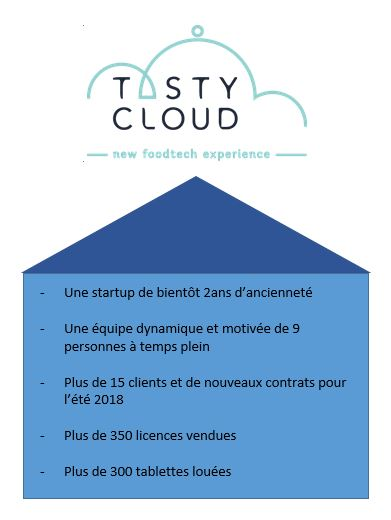
\includegraphics[width=75mm,scale=0.5]{tastystat.JPG}
  \caption{Les chiffres de l'entreprise}
  \label{fig:boat1}
\end{figure}

\subsection{Fonctionnement de l'entreprise}

Tastycloud est une solution clé-en-main. En plus du logiciel sur tablette, l'entreprise fournit divers services tels que :

- L'écoute du besoin client et le développement de fonctionnalités suivant leurs besoins. Le client est constamment mis à contribution dans l'évolution de la solution et le processus de développement étant une partie prenante importante.

- Configuration de la carte à l'aide d'un back office (qui sera présenté plus tard) côté restaurateur qui lui permet de gérer sa carte. Il peut rajouter des produits des formules, des conditions (carte du midi, carte du soir), des options. Ce back office permet aussi au restaurateur d'avoir des statistiques sur ses ventes et les consultations des clients.

- Photographie professionnelle des plats, un photographe professionnel est dépêché sur place pour shooter la totalité de la carte. Bien sûr cela est facultatif si le restaurateur veut prendre ses photos lui-même.

- Traductions des menus,. Comme pour les photos, des professionnels traduisent les menus selon les langues choisies par le client.

- Installation de la solution dans le restaurant (tablettes, espace de rechargement, paramétrage et formation).

- Mise à jour automatique du logiciel lors de la mise en production de nouvelles fonctionnalités.

- L'hébergement des données et data sur le cloud

Tastycloud fournit aussi une assistance aux restaurants toute la semaine et le week-end si besoin ainsi que des assurances vol et casse sur les tablettes. Le service est facturé à 1,50\euro/jour par tablette. Il y a aussi des frais d'installation.
La startup compte beaucoup sur son réseau et les salons autour du foodtech et digital pour trouver de nouveaux clients. Elle s'adonne aussi à la prospection à Paris et à la communication sur les réseaux sociaux.

\subsection{Le logiciel}

Pour bien comprendre de quoi nous parlons, faisons une petite présentation du logiciel d'un point de vue client :

\begin{figure}[!htb]
  \centering
  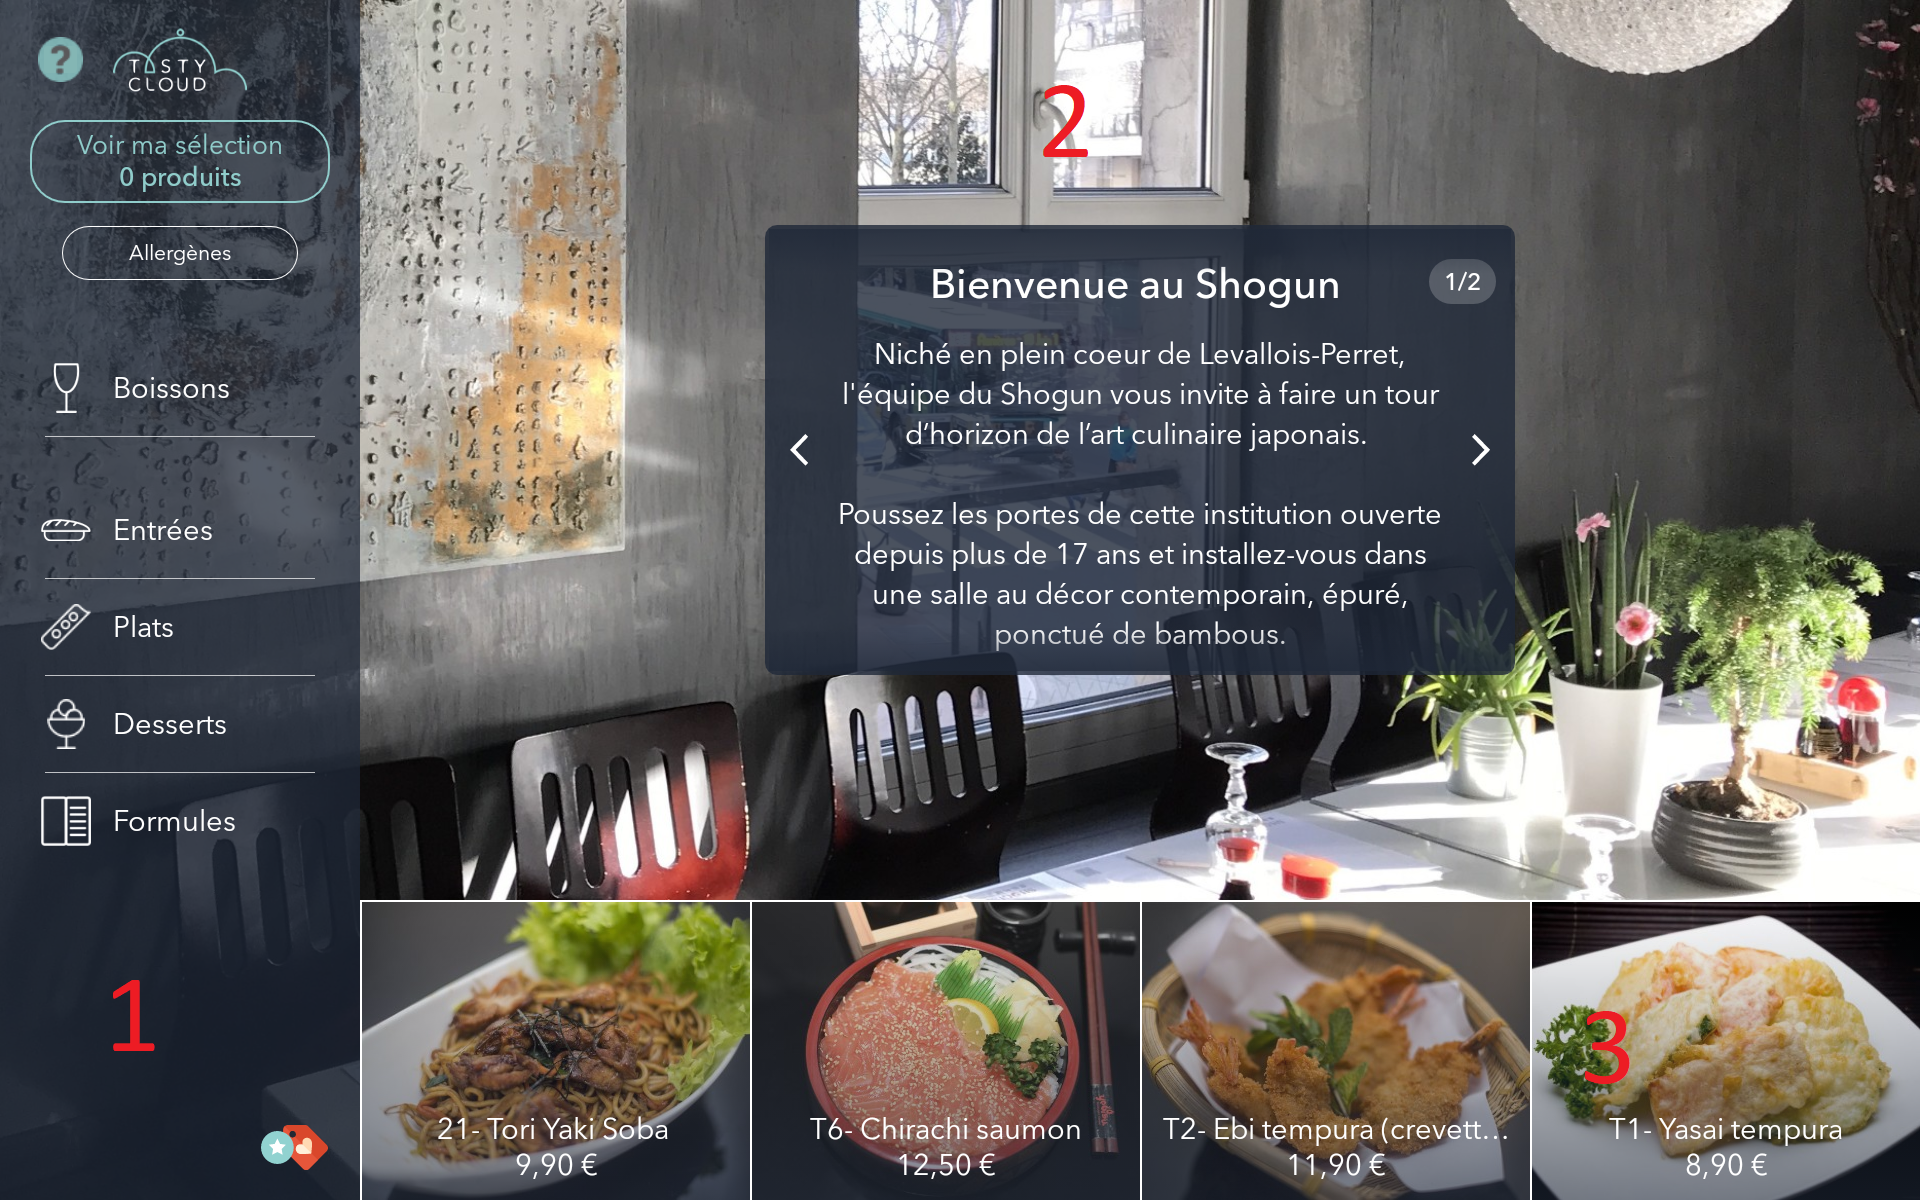
\includegraphics[width=105mm,scale=0.5]{home_tastycloud.png}
  \caption{Le menu "Home" de l'application}
  \label{fig:boat1}
\end{figure}

Voici la page d'accueil d'un restaurant (ici le Shogun). C'est la première page sur laquelle tombe le client. Si nous décomposons l'accueil en 3 rectangles délimités sur la capture d'écran par les numéros un, deux, trois en rouge nous pouvons dire que :

- Le 1 désigne le menu sur lequel le client peut aller chercher ses produits, ses formules ou sa sélection. Comme nous pouvons le voir les produits sont classés par type (boissons, entrées ...). Nous pouvons aussi avoir le choix des langues en bas à gauche mais cette option n'est pas disponible sur ce restaurant. Il y a aussi une option pour les allergènes qui est normalement obligatoire dans les restaurants. La sélection et les allergènes s'ouvrent dans des pop-ups. Pour ce qui est du bouton en haut à gauche il s'agit d'une fonctionnalité que j'ai moi-même développée et nous aurons par conséquent l'occasion de voir tout ça ultérieurement.

- Le 2 est une page de présentation, c'est sur ce rectangle et le 3 que les sous menus vont s'ouvrir (visible sur la capture d'écran ci-dessous) et que l'on va pouvoir naviguer dans l'application.

- Le 3 représente les suggestions de l'établissement, c'est le restaurateur qui choisit les produits qu'il veut mettre en avant sur sa page d'accueil pour avoir une meilleure visibilité des clients.

\begin{figure}[!htb]
  \centering
  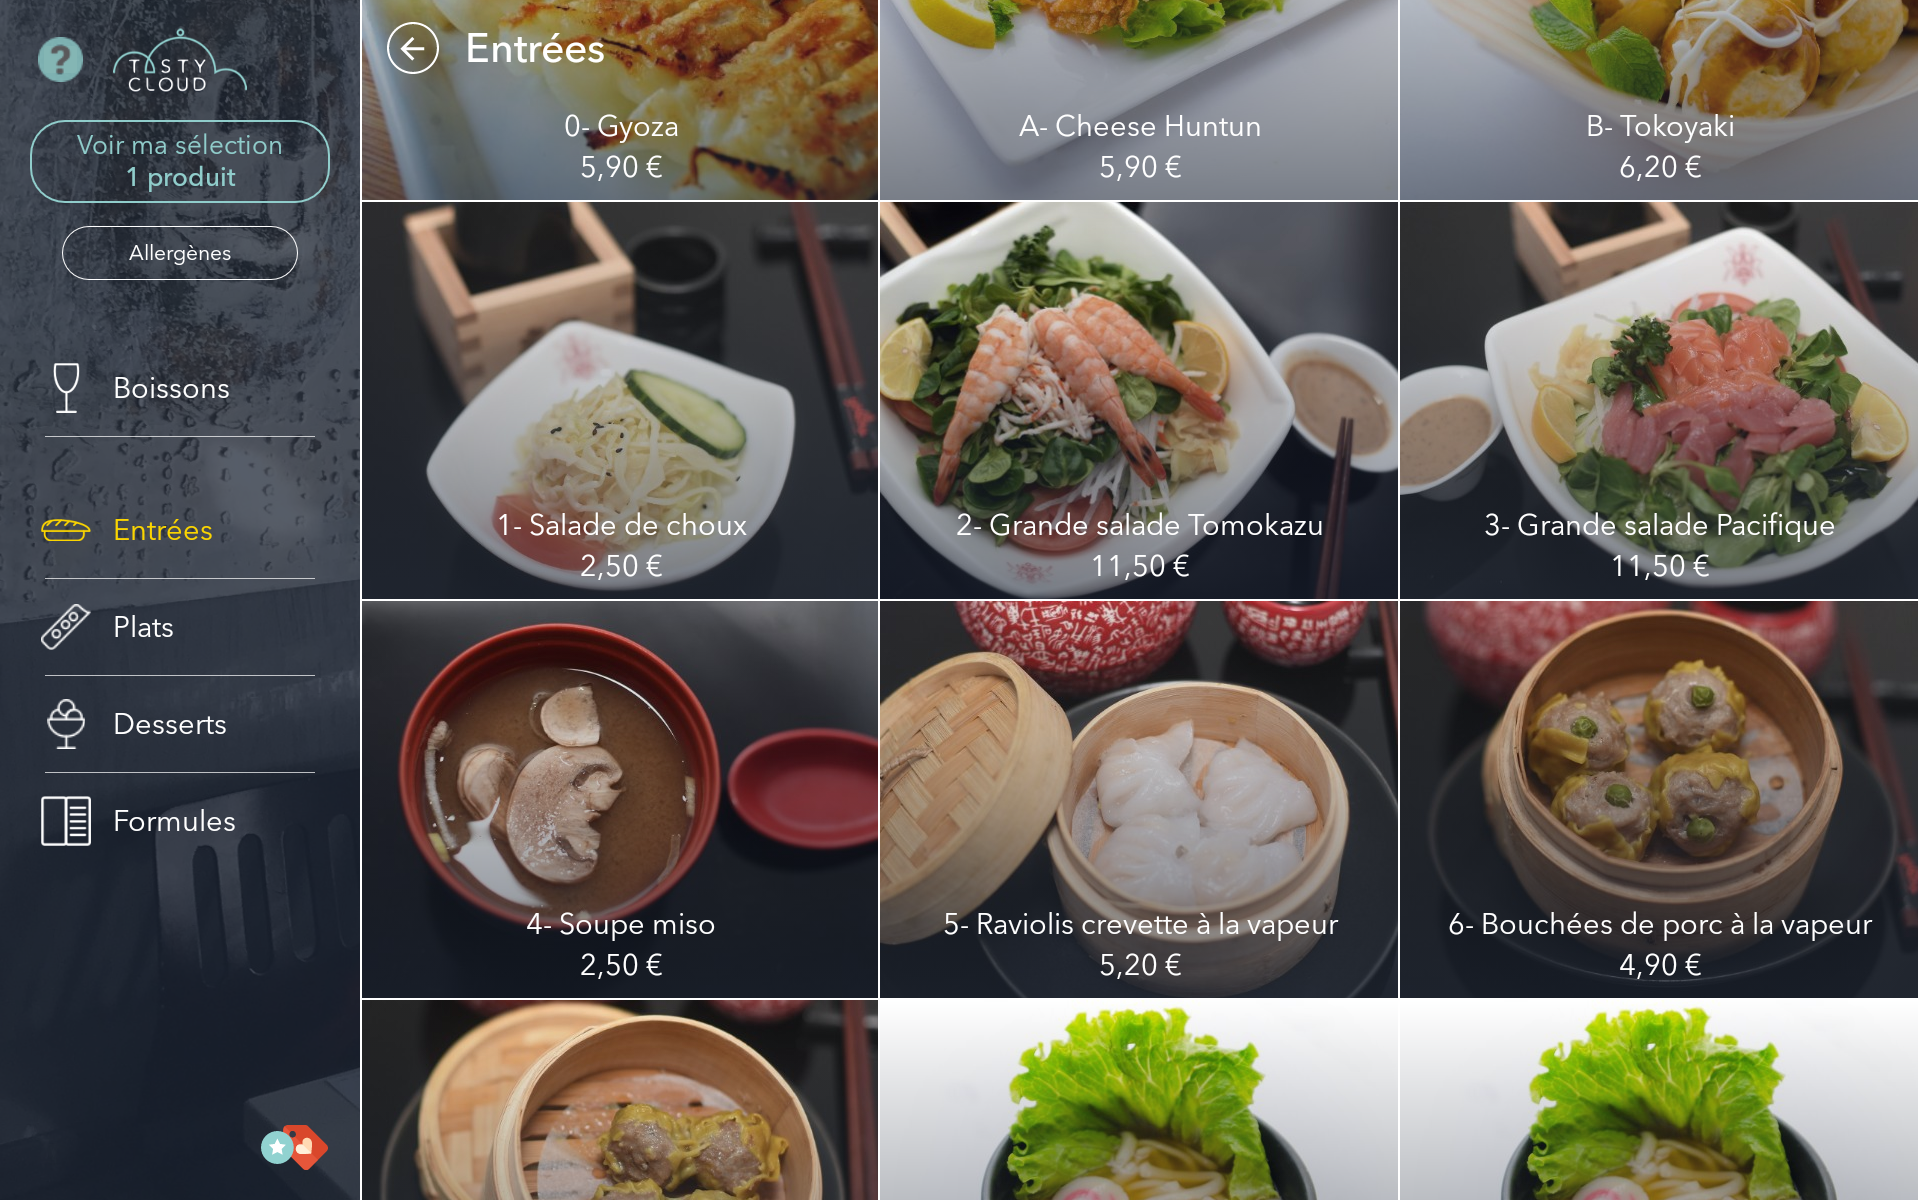
\includegraphics[width=105mm,scale=0.5]{entree_tastycloud.png}
  \caption{Ouverture du menu "Entrées" sur l'application}
  \label{fig:boat1}
\end{figure}

\subsection{Mon poste de travail}

J'ai donc effectué mon stage au siège de Tastycloud dans le 15ème arrondissement à Paris. La société est composée de plusieurs pôles : technique, commercial, opérationnel et marketing. J'ai logiquement travaillé dans le pôle technique avec mon tuteur et d'autres stagiaires. C'est le plus important en terme d'effectifs. L'application grandissant de jour en jour il faut de plus en plus de personnes pour la maintenir (Que ce soit le logiciel ou le back office).\\

L'organisation du bureau est dite en "OpenSpace" ce qui favorise la communication entre les différents membres de l'équipe et qui a pour conséquence d’augmenter la créativité, favoriser l’efficacité au résultat, l'échange d'idées et les suggestions selon les différents points de vue de la startup.

%%% Local Variables: 
%%% mode: latex
%%% TeX-master: "isae-report-template"
%%% End: 

\chapter{Le stage}
\label{chap:lestage}

\section{Présentation du stage}




\subsection{Présentation}

Le stage pour lequel j'ai postulé consiste au développement de l'application Tastycloud sur tablette. J'ai été recruté pour travailler sur différentes missions et accompagner l'évolution de la plateforme avec la mise en place de nouveaux modules et fonctionnalités. Ces dernières peuvent être de nouveaux projets (et donc commencer quelque chose de zéro) ou bien des missions de maintenance par rapport à des retours clients. J'ai par exemple travaillé sur le tutoriel de l'application depuis zéro et ajouté des options utilisateurs disponibles depuis le back office de l'application pour le restaurateur. Bien sûr tout ceci sera détaillé dans les missions de stages.\\

Aujourd'hui la société a de plus en plus de clients et donc de plus en plus de demandes, de maintenance et de suivi clients. Tout ceci génère donc plus de travail et le besoin d'avoir différentes personnes qui travaillent sur l'application. C'est donc dans ce contexte et avec l'encadrement de mon tuteur que mon stage s'inscrit.\\

\subsection{Étude du poste}

Dans un premier temps, il a été important d'être informé sur le contexte du stage que ce soit d'un point de vue technique ou non. C'est pour cela que j'ai eu des formations par rapport à la solution de l'entreprise, comment la présenter et ce qu'elle contient. J'ai également eu des informations sur les différentes fonctionnalités de l'application sur tablette ou le back office, les avantages pour les clients et les restaurateurs. Il a été important de bien comprendre tous les enjeux de la solution et comment elle fonctionnait pour que mon travail reflète au mieux l'identité de l'entreprise.\\

J'ai également eu la présentation du fonctionnement de l'entreprise côté serveur et application à savoir le serveur test et le serveur de production qui servent comme leur nom l'indique l'un à faire les tests et le deuxième pour les clients. Nous avons à notre disposition un back office test. Les clients ont eux un back office séparé du test (nous parlerons de ça dans la partie suivante).\\

J'ai ensuite eu une formation technique après m'être familiarisé avec le fonctionnement de l'application. On m'a expliqué la structure de l'application et son fonctionnement interne. Que ce soit pour la partie graphique, data ou contrôleur. On m'a, la première semaine du stage expliqué tout ceci en détail et répondu à toutes mes questions. J'ai pu ainsi entreprendre mes premières missions plus sereinement. Il a été décidé que d'abord je ferai des petites missions de maintenance pour me familiariser avec la structure de l'application. Ces premières missions étaient diverses et touchaient surtout la partie graphique et la partie base de données. Il n'y avait donc à ce moment-là pas de réelle modélisation mais juste des petits ajouts ou correction de bug. Cela à bien sûr été bénéfique pour moi avant de me lancer dans de réels projets.

\clearpage

\subsection{Le logiciel sur tablette}

Nous avons, dans la première partie présenté le logiciel sur tablette d'un point de vue client. Nous allons rentrer plus en détail de ce qui était à ma disposition dans la version "dev" de l'application. Il faut savoir que le logiciel a une version "dev" et une version "prod". J'ai travaillé principalement sur la version "dev" et mon tuteur s'occupait de faire les mises en productions. On peut mettre l'application à jour en changeant son code (donc on a affaire à un changement interne du fonctionnement de l'application) ou bien en ajoutant par exemple des vins ou des desserts etc, que l'on peut le faire depuis le back office (que l'on va présenter dans la partie suivante). Nous avons une fonctionnalité sur l'application pour mettre directement à jour les changements faits sur le back office.\\

\begin{figure}[!htb]
  \centering
  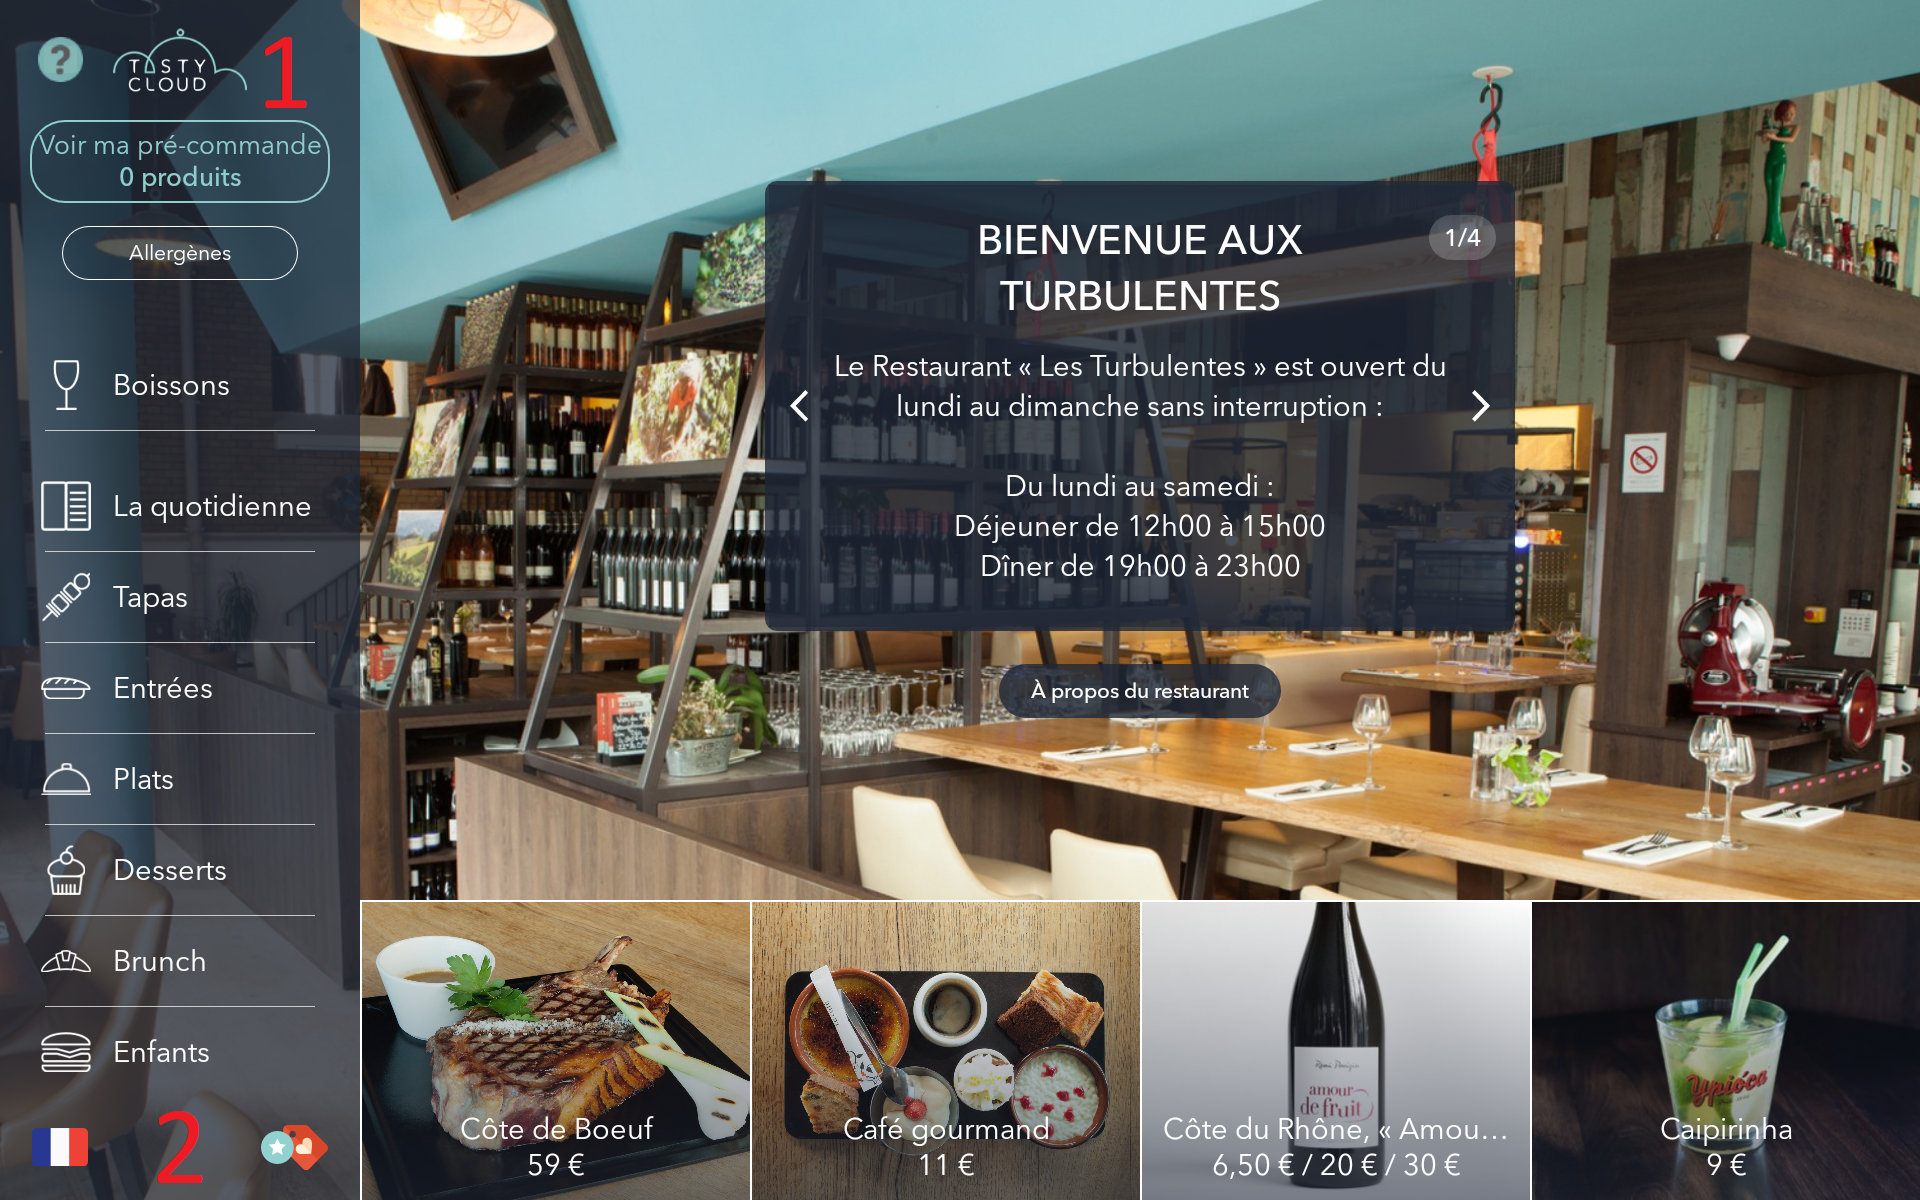
\includegraphics[width=81mm,scale=0.5]{home2_tastycloud.png}
  \caption{Le menu du restaurant "Les Turbulentes"}
  \label{fig:boat1}
\end{figure}

Comme on peut le voir sur la figure ci-dessus, nous avons deux chiffres en rouge. À gauche du 1 c'est le logo de l'application et c'est aussi en faisant ce qu'on appelle un "long click" dessus (donc rester longtemps appuyé sur le logo) qu'on va faire une mise à jour de l'application en synchronisation avec les informations du back office (tout ceci se fait à distance avec le cloud). Pour ce qui est du 2 c'est ici que l'on peut faire un autre "long click" pour accéder à la liste des restaurants sur lesquels on peut naviguer pour faire différents tests (chaque restaurant a ses propres particularités). On peut d'ailleurs vérifier cela avec la présence sur ce restaurant des langues en bas à gauche ce qui n'était pas présent sur le Shogun, le restaurant de l'introduction. On peut voir ci-dessous la page du choix des restaurants, bien sûr ces pages ne sont pas accessibles aux clients du restaurant (voir au restaurateur lui-même).

\begin{figure}[!htb]
  \centering
  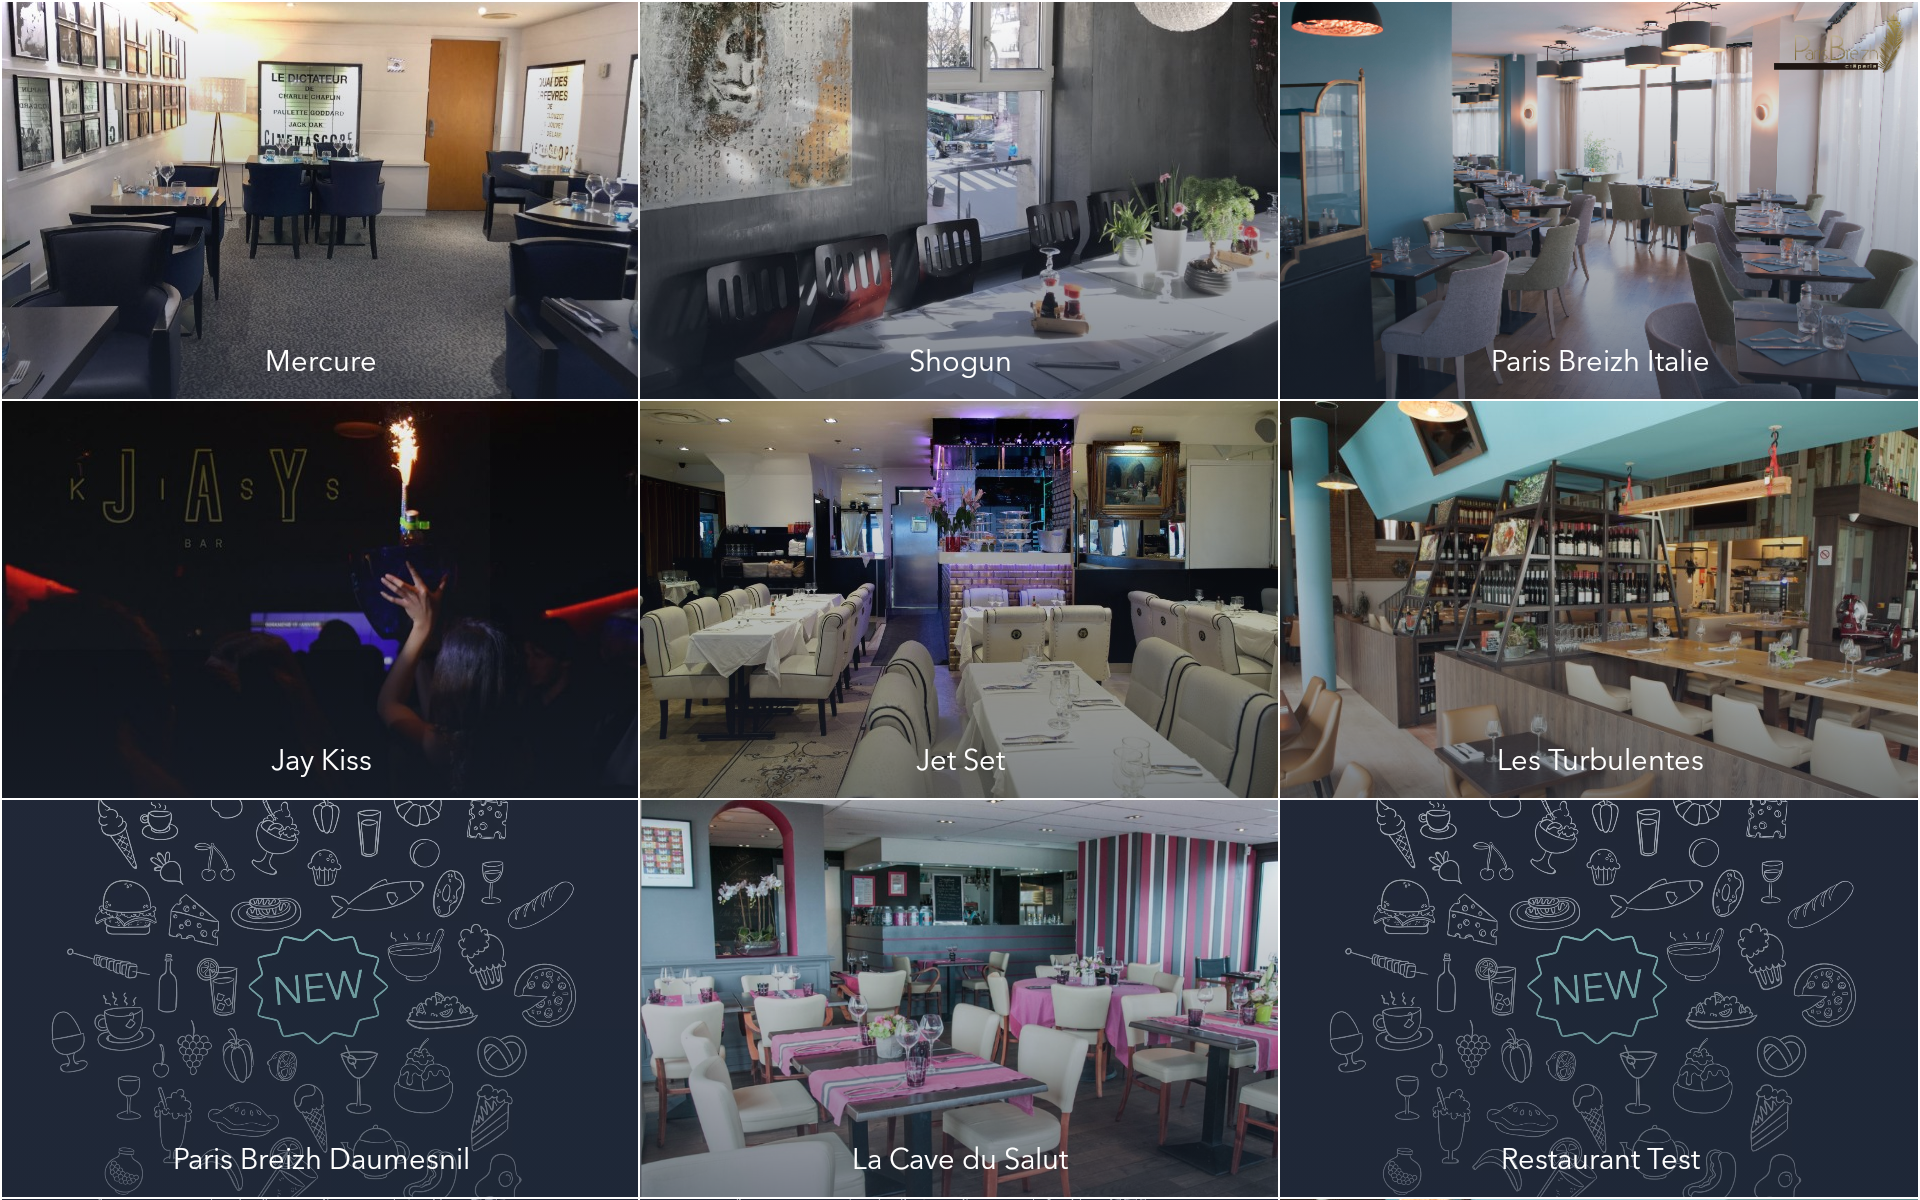
\includegraphics[width=81mm,scale=0.5]{restaurants_tastycloud.png}
  \caption{Page de choix des restaurants}
  \label{fig:boat1}
\end{figure}


\clearpage
\subsection{Le back office}

Le back office est un point essentiel de l'application. C'est ici que sont centralisées toutes les données du restaurant, que ce soit les plats, les boissons, les options, les menus, les descriptions etc... Ce back office est surtout utile pour le restaurateur, c'est avec ce dernier qu'il va pouvoir mettre par exemple à jour sa carte. Comme pour l'application sur tablette, il y a un back office test et prod. Le test est lié à l'application "dev" sur tablette et en toute logique le prod et lié à l'application prod sur tablette. Voyons un aperçu du back office (celui de test) :

\begin{figure}[!htb]
  \centering
  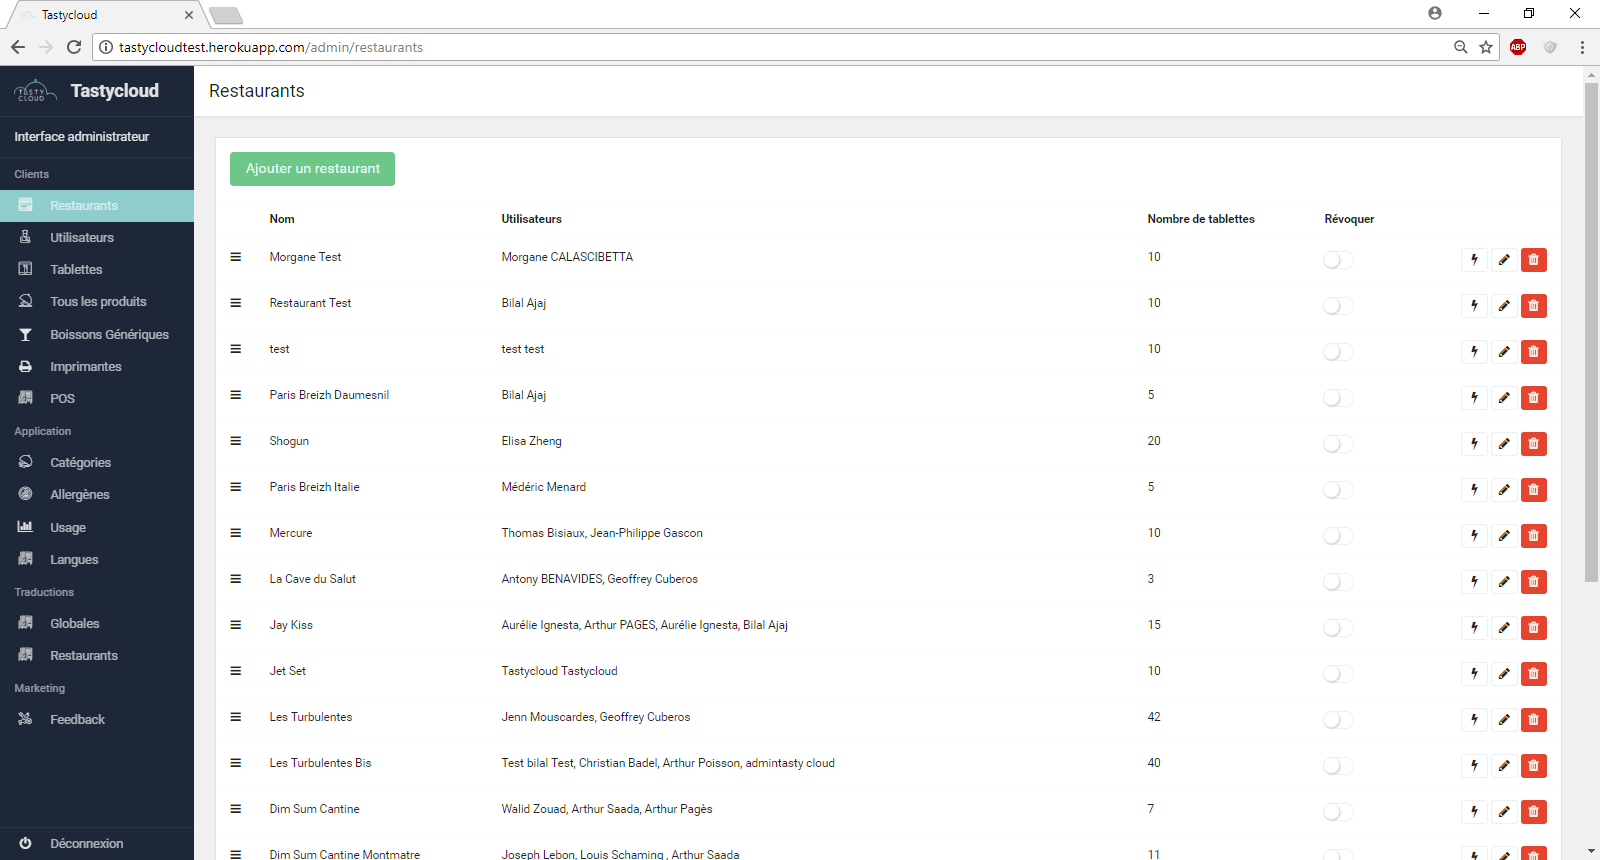
\includegraphics[width=110mm,scale=0.5]{backoffice_tastycloud.png}
  \caption{Back office test}
  \label{fig:boat1}
\end{figure}

Comme nous pouvons le voir sur la figure ci-dessus, le back office contient un menu à gauche et la liste des restaurants dans la fenêtre à droite. C'est sur ce back office que l'on peut par exemple rajouter des tablettes et les affilier à un restaurant. Pour cela on peut cliquer sur l'édition d'un restaurant (bouton à gauche des trois boutons sur la droite d'un restaurant) et par exemple y ajouter de nouvelles tablettes, une nouvelle formule, de nouvelles traductions etc...

\begin{figure}[!htb]
  \centering
  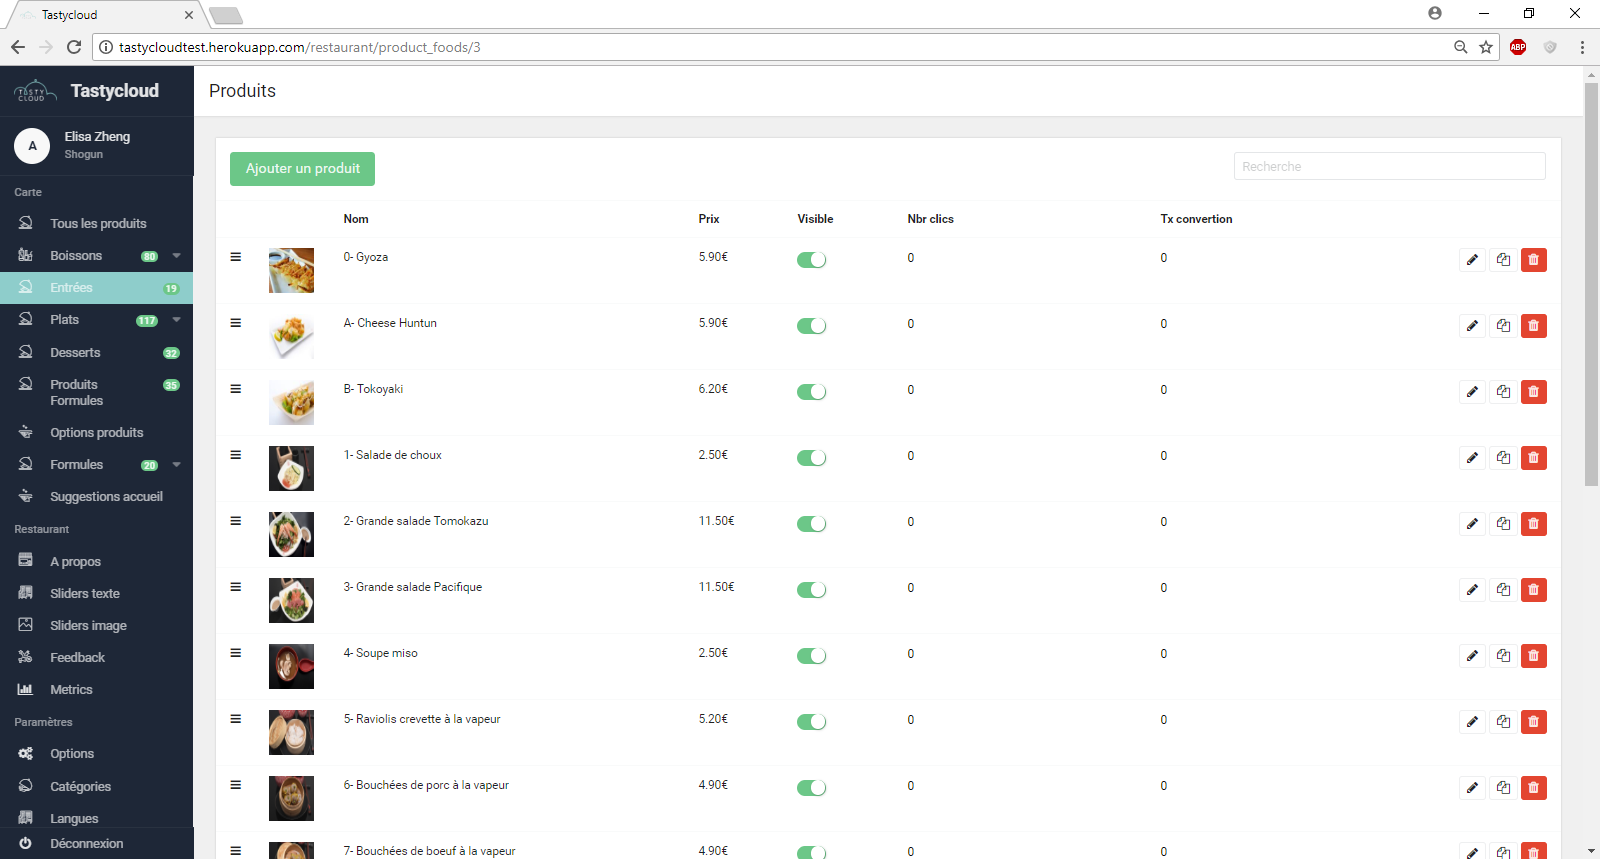
\includegraphics[width=110mm,scale=0.5]{backoffice2_tastycloud.png}
  \caption{Restaurant "Shogun" dans le back office test}
  \label{fig:boat1}
\end{figure}

\section{Technologies et outils utilisés}

\subsection{Android Studio et languages}

L'IDE utilisé pour le développement sur tablette a été Android Studio, nous n'avons pas utilisé d'émulateur puisque les tablettes pour les tests sont fournies. Par rapport au moteur de production (pour builder l'application) nous utilisons Gradle. Les langages utilisés ont principalement été Kotlin et le XML. Kotlin est aujourd'hui un langage supporté officiellement par Android et proche de JAVA. On peut en effet convertir du JAVA en Kotlin (ça ne marche pas tout le temps mais ça existe). Il est intéropérable avec JAVA, qui est le premier langage supporté par Android. Kotlin est un langage récent mais qui propose des avantages pour la sécurité et l'extensibilité du code. Il a en effet des fonctionnalités intéressantes en termes de nullabilité et d'immutabilité. Pour la partie graphique c'est XML qui est utilisé, un langage de balisage qui permet une facilité de lecture et de conception en terme d'arborescence d'éléments. Toutes les vues (éléments qui composent les pages) sont donc définies en XML.\\



\begin{figure}[!htp]
  \centering
  \begin{minipage}[b]{0.2\textwidth}
    
\includegraphics[width=\textwidth]{logo_androidstudio.png}
    \caption{Logo Android}
  \end{minipage}
  \hfill
  \begin{minipage}[b]{0.2\textwidth}
    
\includegraphics[width=\textwidth]{logo_kotlin.png}
    \caption{Logo Kotlin}
  \end{minipage}
  \hfill
  \begin{minipage}[b]{0.2\textwidth}
    
\includegraphics[width=\textwidth]{logo_xml.png}
    \caption{Logo XML}
  \end{minipage}
\end{figure}

\subsection{Les tablettes}

Pour ce qui est des tablettes ce sont des Galaxy Tab A modèle SM-T580. Le logiciel est essentiellement distribué sur ce modèle et donc la taille (10,1 pouces) est unique. Nous n'avons donc pas besoin de prévoir différentes tailles dans le développement de l'application. Ce sont les tablettes fournies aux clients.

\begin{figure}[!htb]
  \centering
  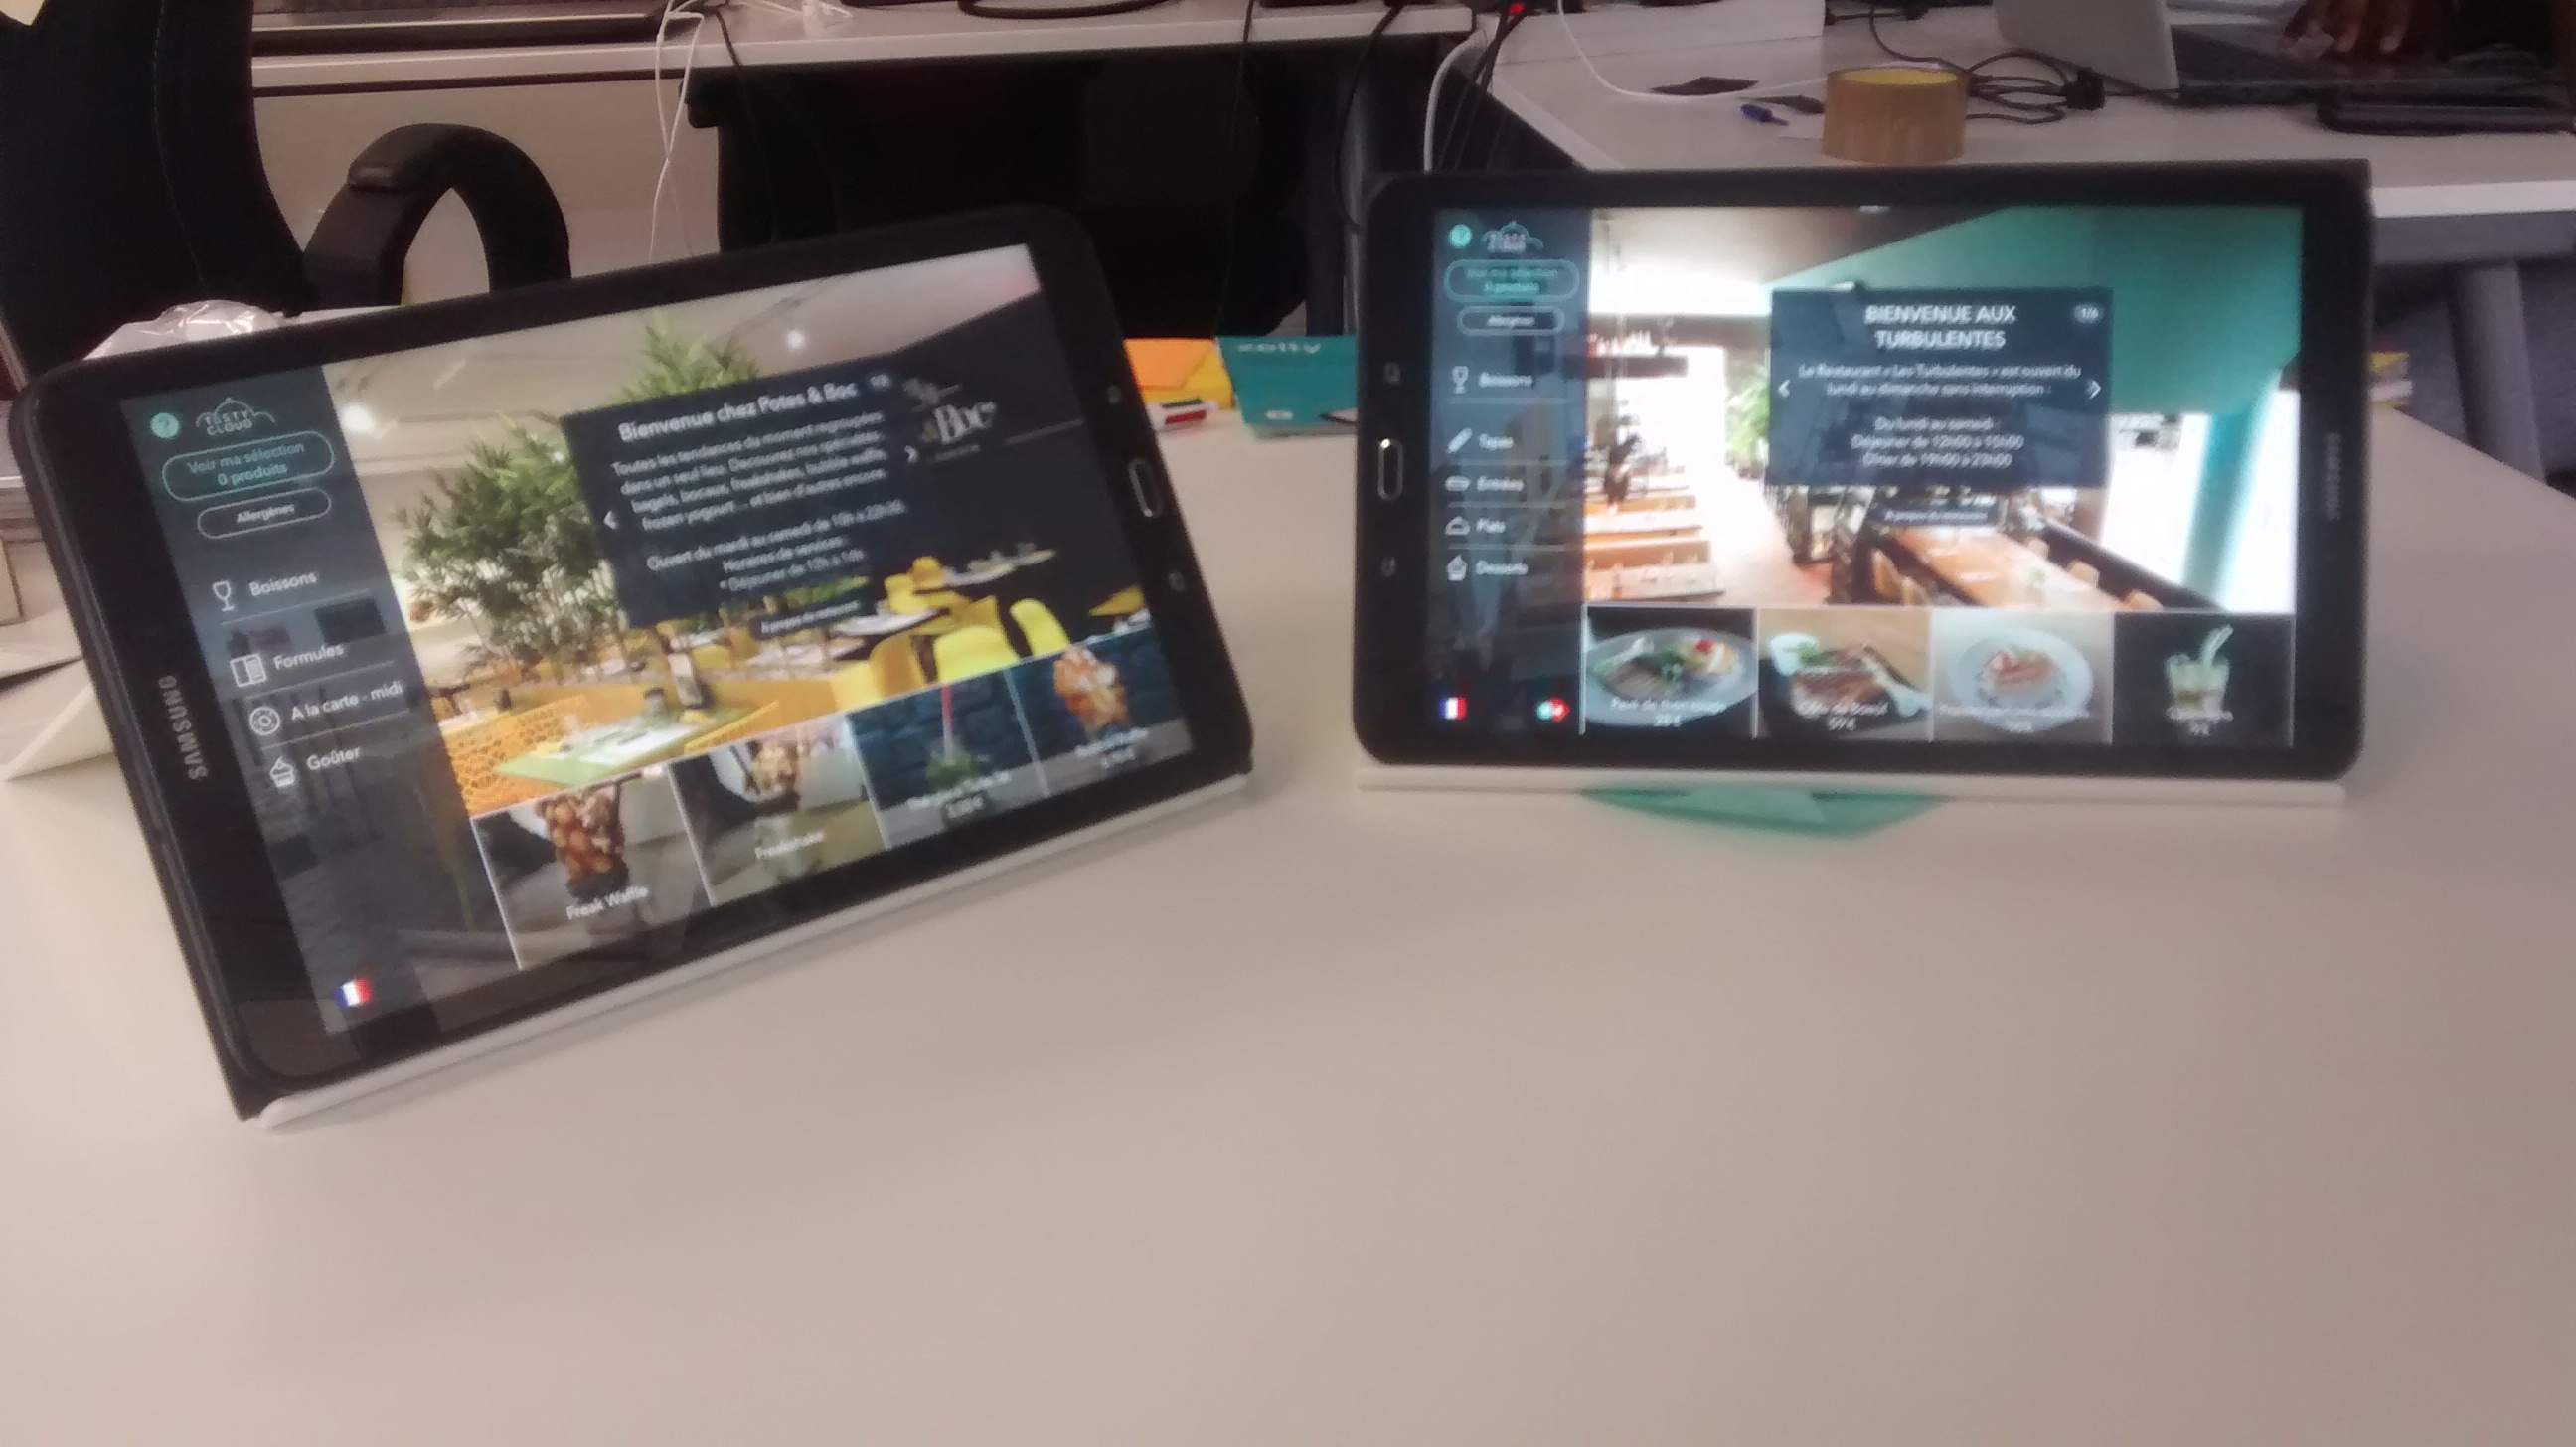
\includegraphics[width=105mm,scale=0.5]{img_tablettes.jpg}
  \caption{Aperçu des tablettes avec l'application}
\end{figure}

\subsection{Git, bit bucket}

Ne travaillant pas seul sur le développement du logiciel et étant amené à travailler en collaboration il a donc été décidé de travailler avec un logiciel de gestion de versions décentralisé tel que git. Ce dernier permet donc à l'équipe de pouvoir échanger des versions du logiciel selon qui travaille sur quoi. C'est ainsi que je peux travailler sur mes propres projets pendant que mon tuteur lui travaille sur autre chose. On met alors en commun ce travail à l'aide de git. Le service web utilisé pour l'hébergement et la visualisation des versions est BitBucket.

\begin{figure}[!htb]
  \centering
  \begin{minipage}[b]{0.25\textwidth}
    
\includegraphics[width=\textwidth]{logo_git.png}
    \caption{Logo git}
  \end{minipage}
  \hfill
  \begin{minipage}[b]{0.3\textwidth}
    
\includegraphics[width=\textwidth]{logo_bitbucket.png}
    \caption{Logo bitbucket}
  \end{minipage}
\end{figure}


\subsection{Outils de communication}

Nous avons utilisé divers outils de communication durant le stage, de manière formelle comme avec des réunions ou des points de parcours, ou de manière organisationnelle avec des logiciels. Les principaux outils logiciels utilisés ont été Basecamp pour la mise en place des tâches et l'affectation de tâches. Basecamp est un outil web de gestion de projet qui permet notamment de me donner des "to-do" qui signifie des objectifs à réaliser dans un temps donné. Chaque tâche peut être plus ou moins complexe et le logiciel permet de communiquer et "taguer" des gens sur cette tâche. C'est un outil pratique car il donne la possibilité de communiquer facilement avec toute l'équipe sur un point donné.

Pour le cas de Basecamp, ce dernier permet de communiquer notamment avec la partie non technique de l'entreprise (par exemple pour communiquer sur des aspects graphiques). Pour l'aspect purement technique nous avons utilisé Slack. Nous avions notamment des channels par rapport à la partie Android et NodeJs.

Enfin dans un souci pratique nous avons également utilisé Whatsapp si nous devions communiquer rapidement et par téléphone lorsque mon tuteur était en déplacement par exemple.

\begin{figure}[!htb]
  \centering
  \begin{minipage}[b]{0.2\textwidth}
    
\includegraphics[width=\textwidth]{logo_basecamp.png}
    \caption{Logo Basecamp}
  \end{minipage}
  \hfill
  \begin{minipage}[b]{0.2\textwidth}
    
\includegraphics[width=\textwidth]{logo_slack.png}
    \caption{Logo Slack}
  \end{minipage}
    \hfill
  \begin{minipage}[b]{0.2\textwidth}
    
\includegraphics[width=\textwidth]{logo_whatsapp.png}
    \caption{Logo Whatsapp}
  \end{minipage}
\end{figure}



%%% Local Variables: 
%%% mode: latex
%%% TeX-master: "isae-report-template"
%%% End: 
\chapter{Les missions}


\section{Missions importantes}
\subsection{Remise en place de l'affiliation}


Ma première mission importante de ce stage a été de remettre en place le système d'affiliation de table du logiciel. L'affiliation est optionnelle et est choisie par le bon vouloir du restaurateur. À mon arrivé côté client voici comment marchait l'affiliation : 

- Un clic long ouvrait sur l'état de la table (sur une table ouverte), un clic simple fermait la table, la table s'ouvrait dès l'instant où un plat était commandé ou choisi.

Et l'objectif de cette mission était de suivre ce schéma d'utilisation :

- Un clic long ferme la table et demande le nombre de convives, un clic simple sur une table ouverte rouvre la table avec l'état. Pour finir la table s'ouvre dès lors que l'on a fait un clic simple sur une table fermée et choisi le nombre de convives.

Pour illustrer mes propos voici des captures d'écrans des deux pages d'affiliation :

\begin{figure}[!htb]
  \centering
  \begin{minipage}[b]{0.45\textwidth}
    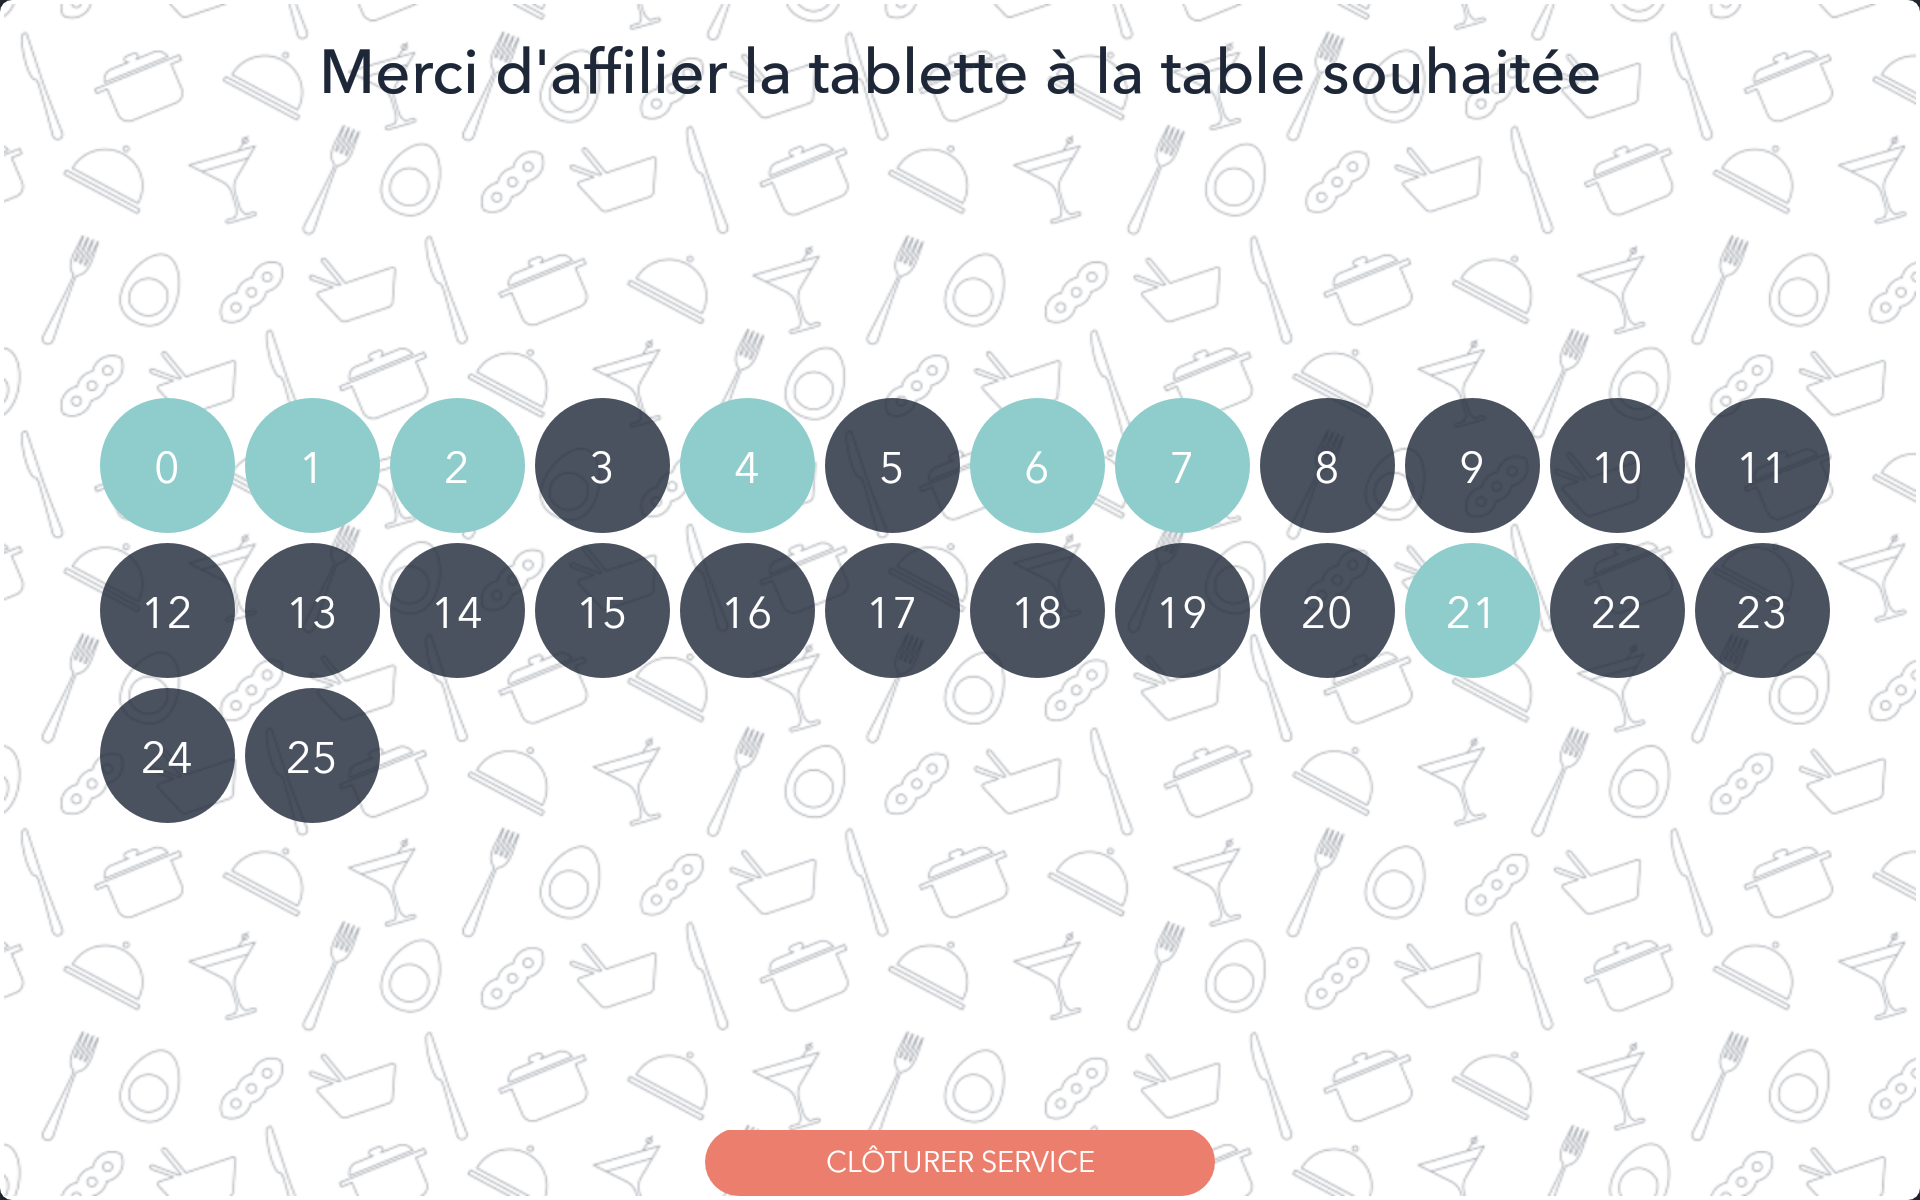
\includegraphics[width=\textwidth]{images/affiliation_table.png}
    \caption{Page d'affiliation de la table}
  \end{minipage}
  \hfill
  \begin{minipage}[b]{0.45\textwidth}
    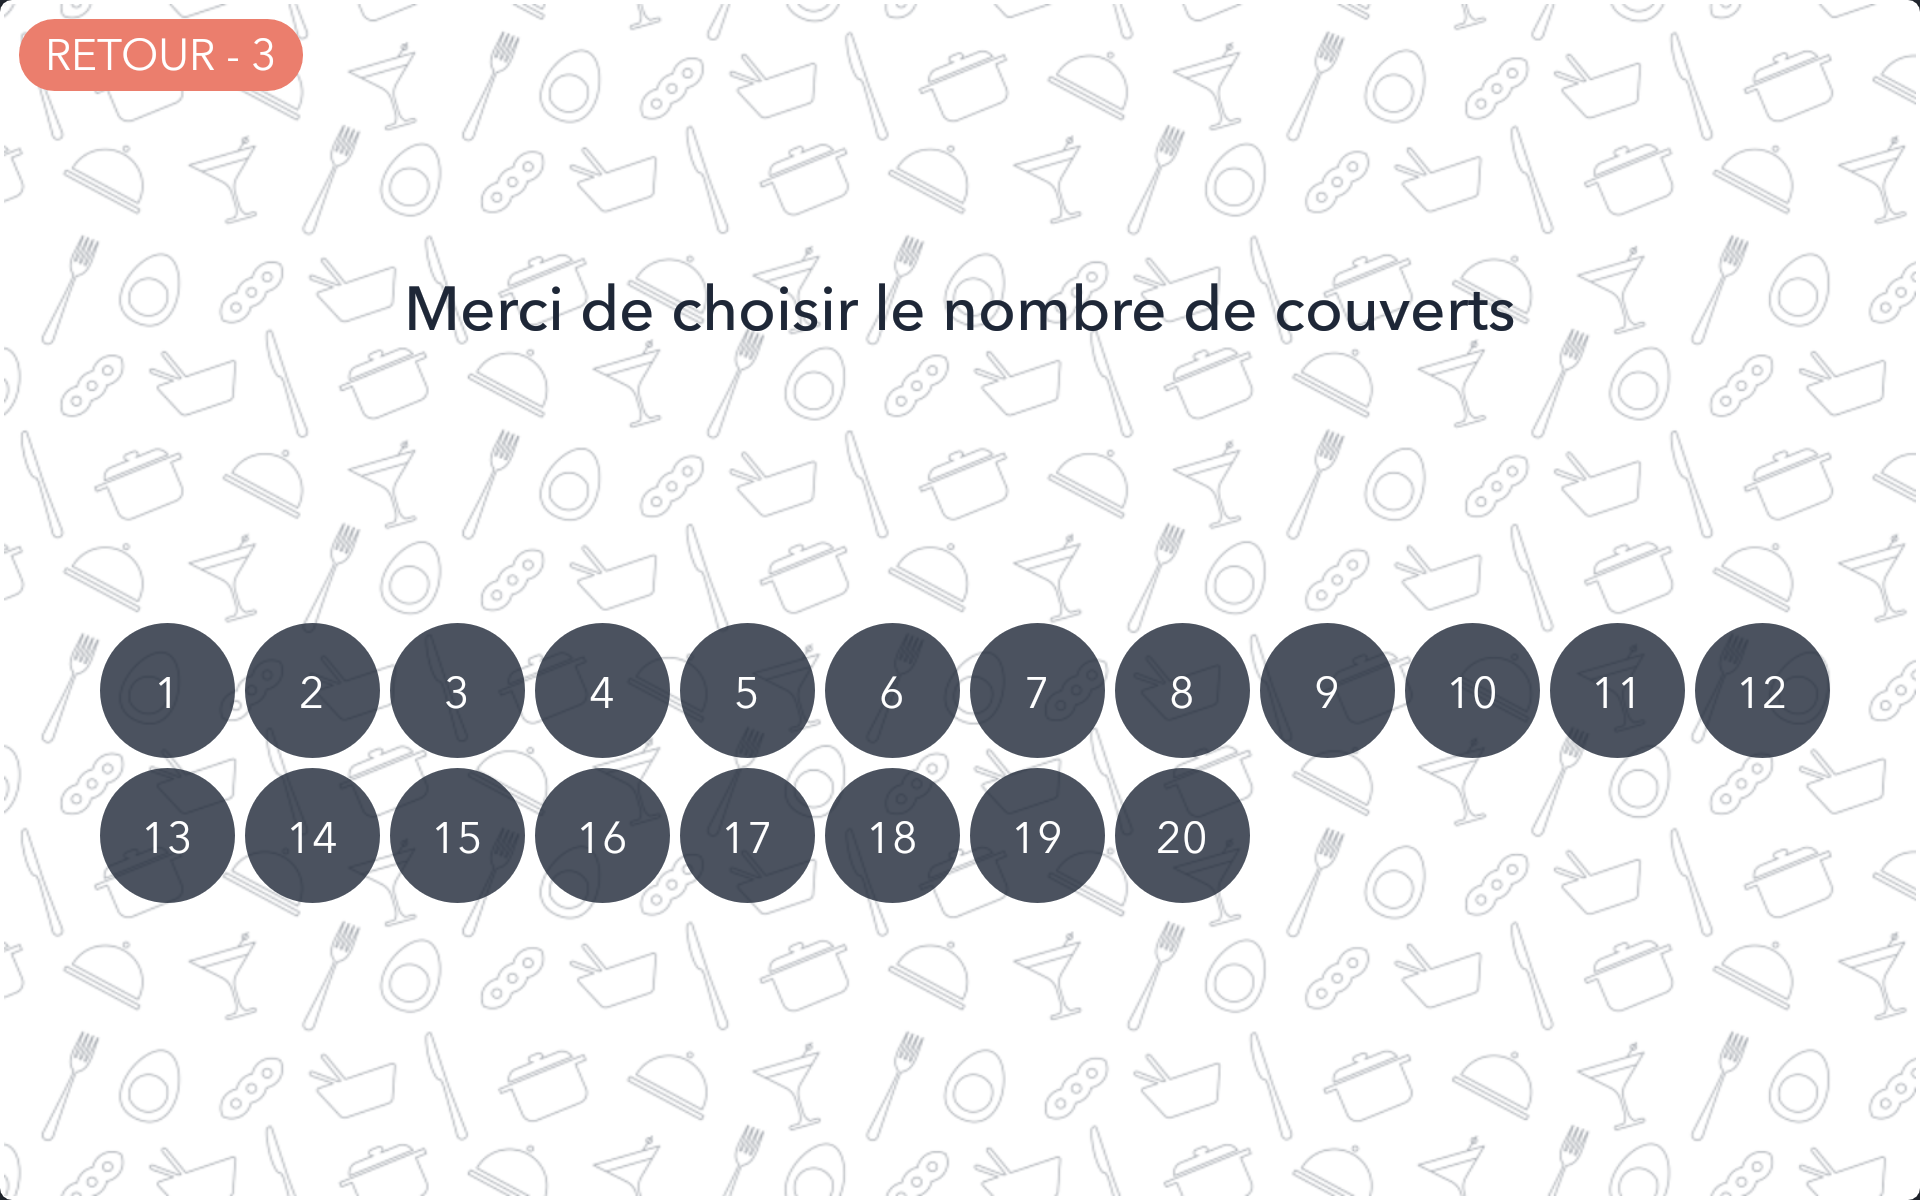
\includegraphics[width=\textwidth]{images/affiliation_convive.png}
    \caption{Choix du nombre de convives}
  \end{minipage}
\end{figure}

Ces deux pages de l'application sont réservées au serveur. C'est lui qui va choisir la table et le nombre de convives. Il a pour cela à sa disposition une liste ou choisir la table dans un premier temps et le nombre de convives dans un deuxième temps. La couleur bleu clair que l'on observe sur certaines tables signifie qu'elles sont ouvertes. C'est sur ces tables que par exemple un clic long entraînerai une fermeture puis une demande du nombre de convives. Les tables sans cette couleur sont donc logiquement des tables fermées.

En plus de cette mission où il a fallu repenser l'affiliation d'un point de vue utilisateur, il m'a été demandé de repenser complètement la structure existante dans l'affiliation. Plus précisément, ma mission consistait à utiliser en Android ce qu'on appelle un "RecyclerView" qui est un conteneur de vues (ici les vues sont les ronds que l'on peut voir dans les captures d'écran ci-dessus). En effet, construire une vue peut être une opération lourde et aujourd'hui Tastycloud commence à avoir des clients qui peuvent par exemple avoir des centaines de tables.

\begin{figure}[!htb]
  \centering
  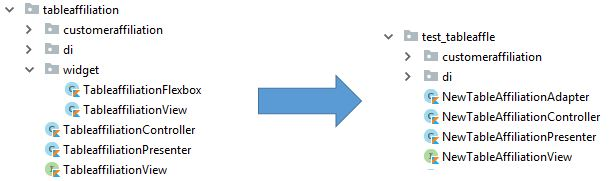
\includegraphics[width=115mm,scale=0.5]{schema_affiliation}
  \caption{Objectif structural de la mission}
  \label{fig:boat1}
\end{figure}

Comme on peut le voir dans la figure ci-dessus à gauche, l'ancienne version possédait une classe "Flexbox" qui utilisait un "FlexboxLayout" qui est donc un outil de mise en page d'Android moins adapté que le "RecyclerView" que je devais moi mettre en place.


Pour le développement de cette structure j'ai donc dû apprendre et réfléchir au fonctionnement du RecyclerView. J'ai dans un premier temps, fais des tests sur la structure déjà existante côté utilisateur, puis j'ai commencé à changer le XML pour mettre en place le ReyclerView. Un premier problème s'est posé quand j'ai compris que je ne devais pas utiliser la même structure qu'avant ce que j'avais fait naïvement dans un premier temps. C'est à dire utiliser un répertoire widget ou j'aurais mis "TableaffiliationRecycler". Après m'être renseigné sur internet et à l'aide de mon tuteur, j'ai compris que le "RecyclerView" a un attribut "adapter". Ce dernier sert à faire la liaison entre le RecyclerView et le contrôleur. Le contrôleur contiendra les logiques précédemment définies à savoir les clics longs et courts et leurs actions ainsi que la création des listes d'éléments qui seront passés à l'adaptateur.

Il a donc fallu créer : 

- Un contrôleur qui contiendra la logique utilisateur et qui créera la liste de tables en fonction de leurs statuts (ouvert, fermé) appelés depuis la base de données de l'application.

- Un adaptateur qui sera en attribut du RecyclerView et qui contiendra la liste des tables.  C'est dans ce dernier que les tables seront traitées une par une pour donner l'effet visuel de table ouverte ou non (rond bleu clair ou non)

- Un presenter qui fera le lien avec la base de données. Ce sera lui qui remontera les informations dans le contrôleur. Le contrôleur héritera d'une interface "View" qui elle contiendra les fonctions appelées par le presenter (en asynchrone).

Bien évidemment, après ce travail de modélisation il faut le réaliser. Heureusement, une structure similaire existait déjà pour une autre fonctionnalité dans l'application, j'ai pu m'en inspirer pour ensuite mettre en place la propre logique de l'affiliation. Seulement, j'ai dû aussi m'inspirer de ce qui existait déjà pour l'affiliation et plusieurs problèmes ont été rencontrés. Le principal a été de convertir toute la logique du Flexbox (donc sur la figure précédente le "TableaffiliationFlexbox") dans le contrôleur.  Ce dernier s'occupait d'ajouter les vues (donc les tables) et de leur attribuer une couleur selon qu'elles étaient ouverte ou non. La première étape à déjà été de construire la liste des tables dans le contrôleur. Pour cela, mon tuteur a décidé de créer une nouvelle table dans la base de données "Table" et d'utiliser un nouveau modèle "TableInformation" qui aura comme attribut le nombre de tables maximum du restaurant et la liste des tables ouvertes (Les éléments de la liste c'est donc par rapport à la nouvelle table créée). Nous avons décidé avec mon tuteur cette solution qui sera beaucoup plus simple pour construire la liste des tables par rapport à ce qui a été fait précédemment pour contrôler ce qui est ouvert ou non. 

Relativement à ce qui a été dit sur le presenter, c'est un cas typique de son utilisation. Lors de l'appel du contrôleur dans l'application une fonction est appelée ("onAttach" dans Android). C'est celle-ci qui est appelée quand le contrôleur est associé à la page courante affichée sur l'application. C'est aussi dans cette dernière que nous allons appeler les fonctions du presenter. Dans notre cas courant voilà ce qui a été fait : Le presenter appelle une fonction dans le OnAttach, ce dernier rappelle une fonction de la vue de manière asynchrone en lui passant un paramètre (donc TableInformation). Cette fonction est définie dans le contrôleur. Le presenter s'occupe lui de faire l'appel à la base de données et à récupérer les informations. Le contrôleur traite TabeInformation dans sa fonction, créé la liste et l'a passe à l'adaptateur. Nous pouvons faire un schéma de ce fonctionnement pour mieux comprendre (un diagramme UML est aussi disponible en annexe).

\clearpage


\begin{figure}[!htp]
  \centering
  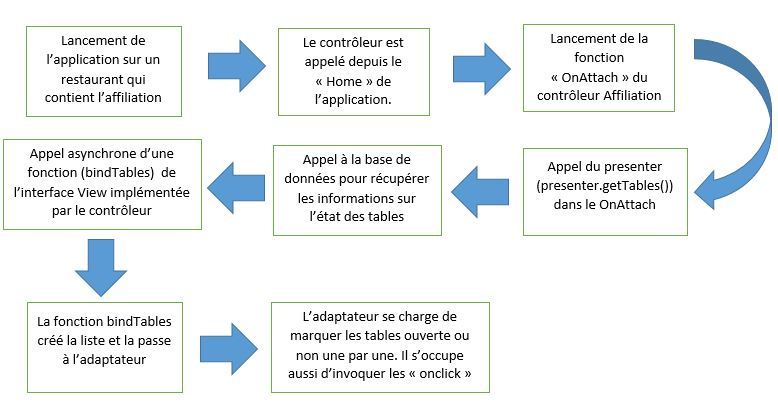
\includegraphics[width=115mm,scale=0.5]{schema2_affiliation}
  \caption{Chemin du programme pour l'affichage des tables}
  \label{fig:boat1}
\end{figure}

Pour ce qui est du presenter il aura des fonctions auxquels nous feront ce qu'on appelle une souscription pour que ce soit asynchrone. Par exemple getTables aura la forme suivante :

\begin{lstlisting}[frame=single]  % Start your code-block
    
    fun getTables() {
        repository.getAllTables()
                .subscribe{ view?.bindTables(it) }
                .toDisposables("getTables")
    }
    
\end{lstlisting}

C'est ainsi que marcheront les appels pour récupérer des informations de la base de données dans le contrôleur. Nous aurons des fonctions définies dans l'interface View qui seront utilisées dans le contrôleur. Le paramètre passé contiendra les informations relatives à la base de données et c'est avec ces informations que nous ferons les traitements.\\

C'est avec l'aide de mon tuteur que j'ai pu comprendre comment créer le chemin pour récupérer les informations et faire le lien avec la base de données. Notamment avec la fonction citée ci-dessus et faire le chemin pour le "repository.getAllTables()". Dans la mise en place de la nouvelle affiliation. Nous avons utilisé cette nouvelle table :

\begin{lstlisting}[frame=single]  % Start your code-block
    
open class TableEntity(
        @PrimaryKey
        override var id: Int = 0,
        open var table_information: String = "",
        open var nb_customers: Int = 0,
        open var is_validated: Boolean = false
) : RealmObject(), Indexed<Int>
    
\end{lstlisting}

TableInformation aura elle une List<Table> des tables ouvertes. Par rapport à l'adaptateur, j'ai suivi ce qui a été fait sur d'autres exemples de l'application j'ai donc entrepris de mettre en place le design pattern "View Holder". Il va construire les vues la première fois et ensuite pourra les mettre à jour sans les reconstruire. C'est ceci qui va permettre à la construction de la liste d'être moins lourde. C'est dans ce ViewHolder que seront faites les mises à jour de couleurs, de texte et dans lequel seront invoqués les "onclick". La logique donnée en début de partie sera par contre définie dans le contrôleur. 

\clearpage

Une fois tout ceci mis en place, il a fallu appliquer la même logique pour les convives. Une fois la méthode assimilée sur l'affiliation le travail sur les convives a été plus rapide. Il a fallu instaurer la même logique avec un adaptateur, un contrôleur et un presenter. Contrairement à l'affiliation les vues doivent simplement amener sur le "home" de l'application quand on clic dessus. La construction de la liste est définie par un nombre X de convives maximum et ainsi une liste de X vues sont créées. Nous n'avons pas besoin d'appel à la base de données dans ce cas le nombre est défini autrement.

Si nous pouvons parler de cette mission d'un point de vue graphique, j'ai aussi géré le cas ou le nombre de tables dépasse le cadre donné au RecyclerView. On peut alors dans ce cas tout simplement scroller. Auparavant nous avions un bug graphique et les ronds prenaient tout l'écran. J'ai dû pour cela me renseigner sur les logiques arborescentes d'Android en XML et j'ai donné différents poids aux éléments graphiques : 

\begin{figure}[!htp]
  \centering
  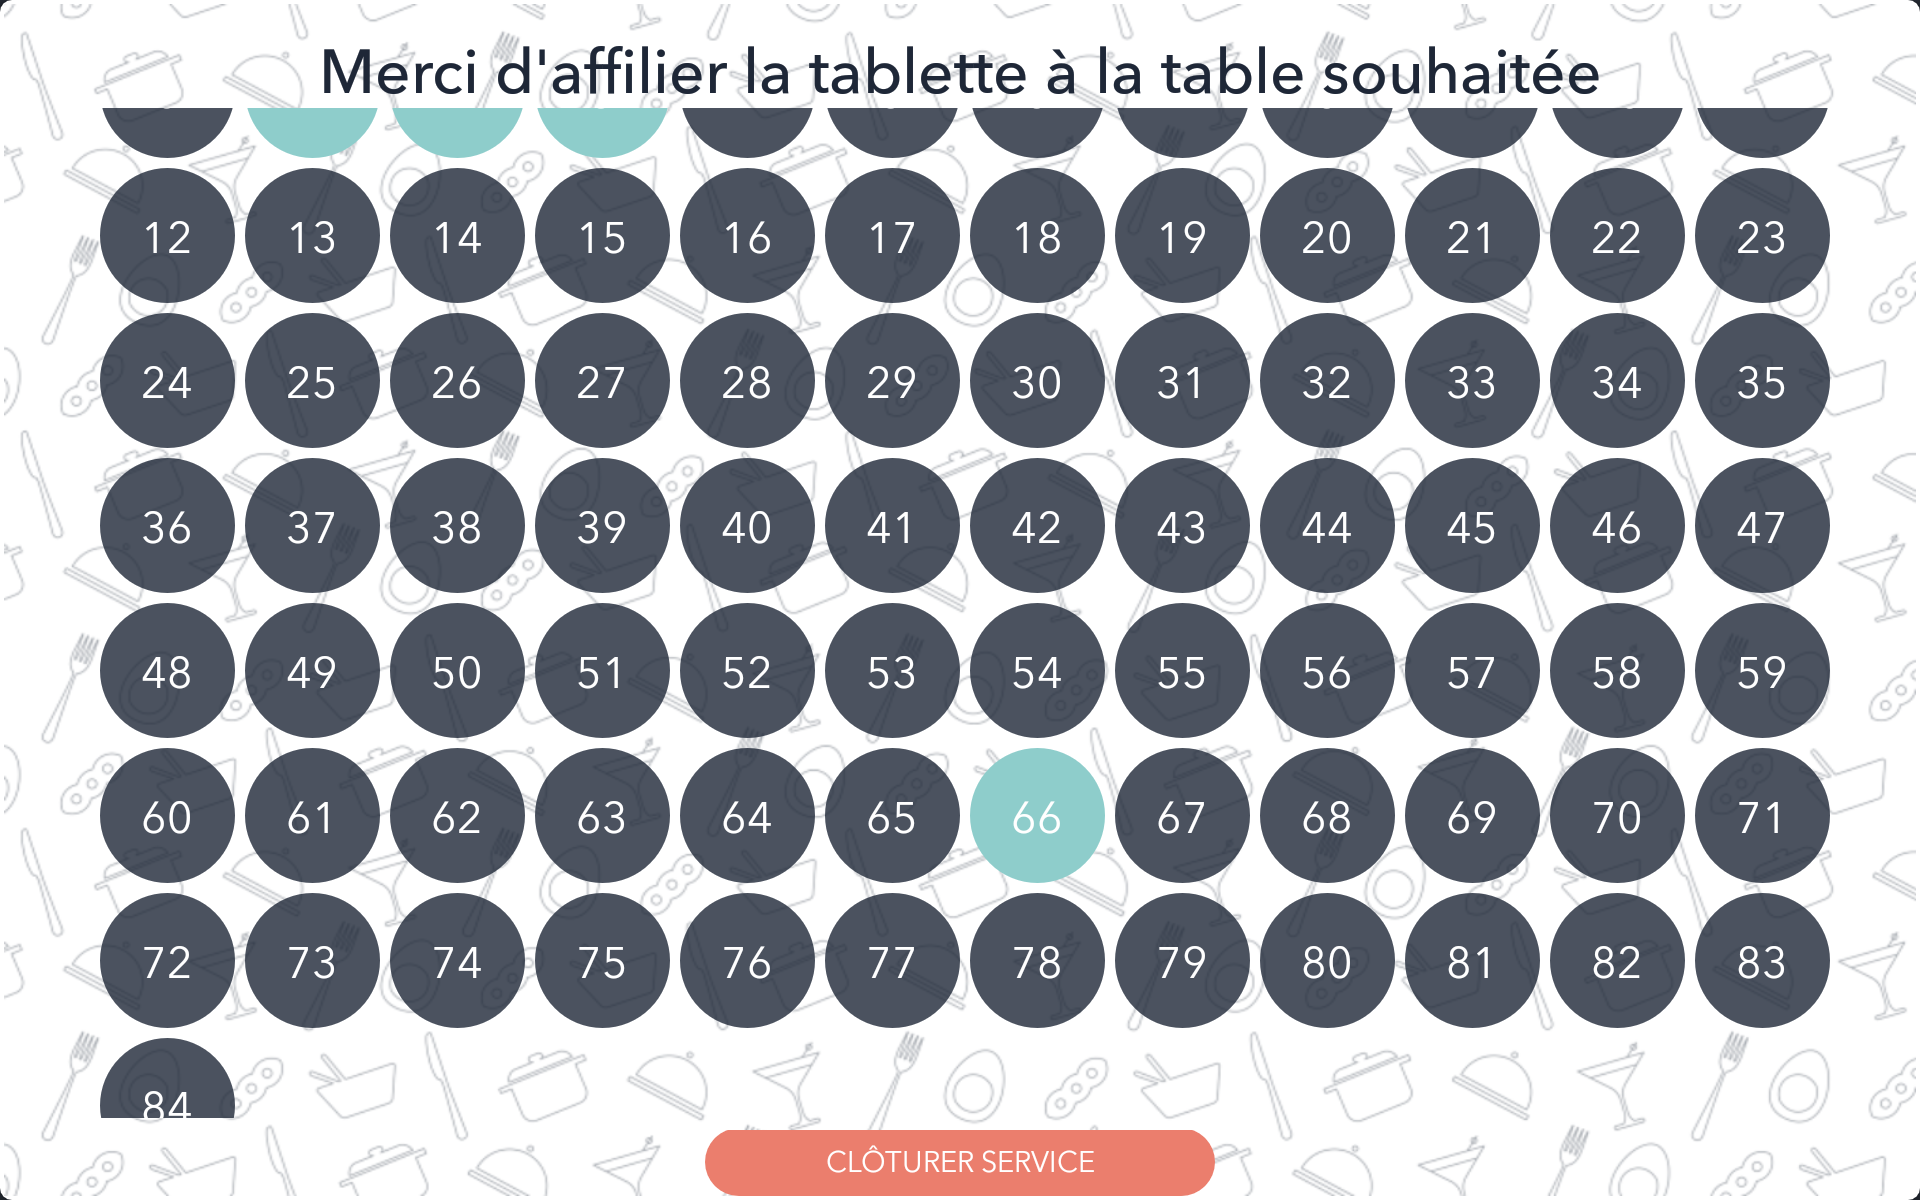
\includegraphics[width=115mm,scale=0.5]{images/affiliation_screen.png}
  \caption{Exemple de restaurant ou le nombre de tables est élevé}
  \label{fig:boat1}
\end{figure}

Comme on peut le voir sur cette capture d'écran, nous pouvons découper la page en 3 vues : Le titre en haut, le RecyclerView (donc le conteneur) et enfin le bouton pour clôturer le service. Pour avoir ce résultat j'ai décidé de donner au conteneur des 3 vues un poids avec l'attribut "WeightSum" et de donner 9/10ème de ce poids au RecyclerView.

Cette mission a surtout été une mission de recherche et d'adaptation d'un modèle à l'autre. La conception et le développement y étaient relativement restreints mais elle m'a permis de bien comprendre comment fonctionne l'application d'un point de vue technique. Elle m'a également permis de bien comprendre certaines subtilités d'Android. C'était la mission la plus technique du stage car très peu visuelle par rapport aux autres. Ce qui n'est pas le cas, par exemple, de la mission suivante où le développement s'est fait de zéro et où il a fallu inventer une nouvelle structure.

\clearpage

\subsection{Tutoriel}

Dès mon entretien l'équipe m'avait parlé d'un projet de didacticiel à mettre en place sur le logiciel visant les personnes moins à l'aise avec la technologie pour leur proposer un parcours ludique qui expliquerait rapidement un chemin d'utilisation de l'application de manière visuelle. Avant mon arrivée, l'équipe a réfléchi aux différentes pop-ups présentes dans le tutoriel et a demandé à des designers de mettre en place une première version sous forme de PNG :

\begin{figure}[!htb]
  \centering
  \begin{minipage}[b]{0.45\textwidth}
    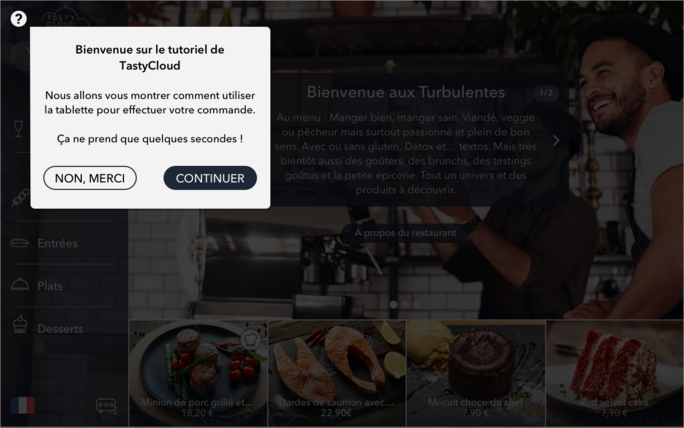
\includegraphics[width=\textwidth]{images/tutoriel_design.png}
    \caption{Première étape du didacticiel}
  \end{minipage}
  \hfill
  \begin{minipage}[b]{0.45\textwidth}
    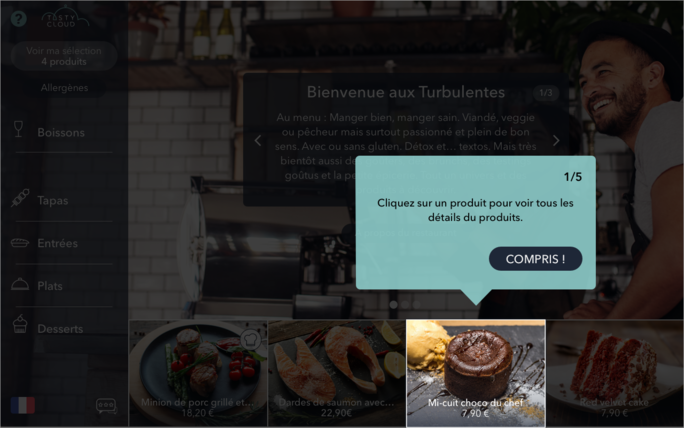
\includegraphics[width=\textwidth]{images/tutoriel_design2.png}
    \caption{Deuxième étape du diacticiel}
  \end{minipage}
\end{figure}

Comme on peut le voir sur les images ci-dessus, le but était de travailler avec des pop-ups et de parcourir l'application. J'avais à ma disposition ces 2 images et les textes à mettre dans les pop-ups pour les étapes suivantes. Le didacticiel étant un nouveau projet j'ai dû dans un premier temps faire des recherches sur quoi utiliser pour mettre en oeuvre une première version. J'ai d'abord décidé de mettre en place le bouton sur la page d'accueil de l'application entre le bord gauche et le logo. Tout ceci se fait dans le XML, j'ai centré le bouton dans l'espace vide entre le logo et le bord gauche. Après cette première étape terminée il a fallu trouver un moyen de créer les pop-ups. J'ai d'abord réfléchi au "DialogBox" d'Android. Cet outil affiche par défaut une fenêtre avec deux boutons "Ok" et "Annuler" et grise le fond. Je me suis vite rendu compte que cet outil n'était pas vraiment fait pour l'utilisation d'un didacticiel car il aurait fallu redéfinir tout le contexte par défaut. Les DialogBox sont plus utiles pour un cas où l'on aura un pop-up qui nous demanderait de cocher des choix ou bien entrer un texte pour un traitement futur ce qui n'était pas réellement le cas d'utilisation ici. Après recherche sur le guide de développeur d'Android je me suis aperçu qu'un autre outil "PopupWinow" répondait plus à mes attentes. Dans le cas du didacticiel nous avons besoin que la pop-up s'affiche, s'efface et se réaffiche assez souvent sans avoir de ralentissement. Avec un DialogBox cela aurait été moins fluide. Le PopupWindow était intéressant car il permet facilement le changement de position (les pop-ups du didacticiel changent de place assez souvent). On peut aussi facilement lui associer un layout (donc une page graphique) dans le XML.

J'ai donc dans un premier temps créé mon layout en XML en reprenant les PNG que l'on m'avait fournis ci-dessus. On a par ailleurs décidé avec mon tuteur qu'il serait mieux de donner la possibilité à l'utilisateur de pouvoir quitter le tutoriel à tout moment. Par conséquent, excepté pour le message d'introduction qui propose déjà un bouton pour quitter, nous avons décidé de mettre un bouton en haut à gauche pour quitter durant les autres étapes du tutoriel. Il a aussi été décidé à ce moment-là de garder la même couleur pour tout le tutoriel et de ne plus utiliser le bleu que l'on peut apercevoir dans la deuxième capture d'écran ci-dessus.

D'un point de vue graphique nous avons donc 3 principaux conteneurs dans le XML du pop-up. Le premier en haut et horizontal qui contient le bouton pour quitter et le compteur pour savoir à quelle étape on est, le deuxième qui contient le texte (titre et texte) qui est vertical et le dernier qui contient les deux boutons.

\clearpage


\begin{figure}[!htp]
  \centering
  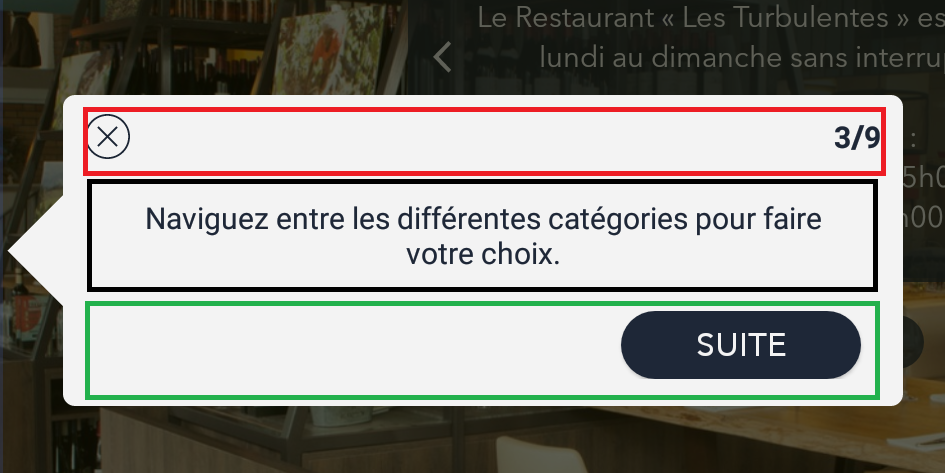
\includegraphics[width=115mm,scale=0.5]{images/tutorial_popup.png}
  \caption{Exemple d'une étape du didacticiel}
  \label{fig:boat1}
\end{figure}

Nous avons par exemple dans l'image ci-dessus décomposé le didacticiel en 3 rectangles qui délimitent les conteneurs définis précédemment. Ce qu'on peut noter c'est que dans certains cas certains éléments graphiques seront rendus invisibles. Par exemple, tout rectangle rouge dans le message de bienvenue du didacticiel est caché. Dans les étapes du tutoriel c'est le titre présent dans le rectangle noir qui est caché et le bouton de gauche dans le rectangle vert.

Une dernière étape dans la mise en place graphique des pop-ups ont été les triangles. On peut dans la capture d'écran en voir un à gauche. Ces triangles peuvent être présents en haut, en bas, à droite, à gauche. J'ai au début pensé à définir un triangle que je pourrais déplacer et retourner en fonction des cas. Cependant c'était une solution loin d'être pratique surtout que l'on peut dans le futur rajouter des étapes. J'ai donc directement défini 4 triangles dans le XML qui se mettaient à chaque fois dans la bonne orientation et au milieu d'un des quatre côtés. Ces quatre triangles sont donc cachés et peuvent être rendus visibles dans le code. C'est une utilisation bien plus simple par rapport à ce que j'avais préconisé dans un premier temps, c'est aussi bien plus simple de réutilisation.

Une fois le côté graphique des pop-ups créé, il a fallu penser à la réutilisabilité du didacticiel. C'est à dire prévoir les cas où il faudrait rajouter des étapes, changer le style graphique etc. Pour cela j'ai décidé de définir ma propre classe qui hérite de PopupWindow et qui aura en attribut les textes, les boutons et les triangles. J'ai pensé à un système où l'on aurait seulement besoin de définir les textes, le nombre d'étapes et les localisations des pop-up sur l'écran pour créer le tutoriel. Pour revenir sur les triangles j'ai par exemple une fonction de cette classe héritée "setTriangle" qui prend en paramètre une "Orientation" soit une énumération qui peut prendre comme valeurs différentes : LEFT, BOTTOM, TOP, RIGHT, GONE. Pour les positions différentes et pour le cas où il n'y a pas de triangles. Cette fonction est simplement appelée selon les différentes étapes et selon l'orientation que l'on souhaite. Cette solution permet par exemple une lecture du code simple si quelqu'un devait reprendre mon travail dans le futur. J'ai aussi pensé à créer deux fonctions, une "startTutorial" qui permet de lancer les éléments graphiques du tutoriel (c'est à dire après avoir appuyé sur "continuer" sur la première pop-up) et une autre fonction "nextStep" qui permet l'incrémentation du compteur, du texte et de la position de la pop-up. Ces 3 éléments étant définis dans des tableaux à l'initialisation.

Une fois que cette première étape a été réalisée j'ai été confronté à un premier problème auquel il a été, dans un premier temps, difficile de répondre. Comme on peut le voir dans les captures d'écrans de la page précédente, pendant que le didacticiel est déroulé le fond de l'application est foncé et les éléments sur lesquels on doit mettre l'accent (par exemple le bouton du tutoriel et un des plats de la barre de suggestion) sont mis, eux, en transparent.

Dans un premier temps il a fallu mettre le fond en foncé. J'ai alors fait des tests sur l'élément qui englobait tous les autres dans la page d'accueil de l'application. Le problème est que cet élément étant parent d'autres éléments fils, changer la couleur de fond ne se verra pas, en effet ses fils vont "prendre le dessus". J'ai alors testé avec l'attribut "foreground" que l'on pourrait traduire par premier plan. Dans ce cas le fond devenait bien foncé mais malheureusement on a fait face au problème que les éléments graphiques ajoutés seront forcément sous le premier plan et donc tous les éléments seront assombris. Il a donc été décidé de faire une nouvelle arborescence. On va dans un premier temps définir un père qui aura un fils qui lui va contenir tous les éléments graphiques de la page d'accueil. Hors de ce fils, on va définir une nouvelle vue qui prendra l'ensemble de la page et qui sera "au dessus" de l'autre vue qui contient tous les autres éléments graphiques. Ainsi sur cette vue on pourra définir les pop-ups et les éléments à rendre plus clair. On peut donner un aperçu de cette arborescence avec le code XML ci-dessous : 

\begin{lstlisting}[frame=single]  % Start your code-block
    
<RelativeLayout
    android:id="@+id/home"
    android:layout_width="match_parent"
    android:layout_height="match_parent">
    
    <FrameLayout... />
    
    <com.tastycloud.ui.home.tutorial.BrightView.../>
    
    </RelativeLayout>
    
\end{lstlisting}

Le RelativeLayout est le père, le FrameLayout contient tous les éléments graphiques de la page et le BrightView sera celui qu'on affichera quand on lancera le didacticiel. Rendre les éléments plus clairs a été un autre problème, il a fallu réfléchir à une solution pour rendre le fond foncé sauf à quelques endroits précis où il devait devenir transparent. J'ai pensé dans un premier temps à créer au dessus du BrightView un "ImageView" (un élément graphique pour les images) et à superposer cet élément sur ceux qu'il fallait rendre plus clair. Seulement, cette solution n'est pas vraiment viable car il faudrait reprendre le même "design" qui existe déjà sur les éléments à rendre plus clair pour pouvoir y mettre l'ImageView. On a donc réfléchi à une solution avec mon tuteur et j'ai après quelques recherches sur internet trouvé un moyen de dessiner des formes (rectangle, rond) à l'intérieur de la "BrightView". Ces formes seraient alors transparentes. Comme on peut le voir dans l'extrait de code "BrightView" est une classe définie dans le projet. Elle hérite de FrameLayout et on va alors pouvoir redéfinir sa fonction onDraw. La fonction "onDraw" va contenir elle comme paramètre un "Canvas" qui lui va contenir les appels qui vont permettre de dessiner sur le BrightView. L'idée est d'ensuite avoir ce BrightView en attribut du PopupWindow défini lui aussi dans le code. Ainsi, on pourra directement définir avec cette classe qui étend de PopupWindow les éléments à éclairer, la forme qu'ils doivent avoir, leur emplacement etc... Pour que l'utilisateur ne passe pas par BrightView toutes les fonctions de BrightView pour dessiner des formes (par exemple "setRoundedRectangle", "setRectangle", "setCircle") sont redéléguées à BrightView dans PopupTutorial (donc la classe qui hérite de PopupWindow). C'est à dire qu'on aura des fonctions de ce type dans PopupTutorial :

\begin{lstlisting}[frame=single]  % Start your code-block
    
    fun setBrightViewRectangle(v: View) {
        brightView.setRectangle(v)
    }
    
    fun setBrightViewCircle(x: Float, y: Float, radius: Float) {
        brightView.setCircle(x, y, radius)
    }
    
\end{lstlisting}

Tout ceci est donc fait dans un souci de réutilisabilité et pour que si un autre utilisateur venait à reprendre ce code, qu'il n'est pas à instancier différents éléments pour par exemple créer une nouvelle étape. Les fonctions définies dans BrightView s'occupent d'affecter les valeurs passées en paramètre puis d'appeler le onDraw qui va dessiner l'élément selon le type défini par une énumération et qui est affecté dans les dites fonctions : 

\begin{lstlisting}[frame=single]  % Start your code-block
    
    override fun onDraw(canvas: Canvas?) {
        
        canvas?.drawColor(mTutorialColor); //couleur de fond
        
        //dessine selon de type (DrawType)
        if (mCx >= 0 && mCy >= 0) {
            when (currentDrawType) {
                DrawType.CIRCLE -> canvas?.drawCircle(...)
                DrawType.RECTANGLE -> canvas?.drawRect(...)
                DrawType.ROUND_RECTANGLE -> canvas?.drawRoundRect(...)
                DrawType.EXTRA_RECTANGLE -> {
                    canvas?.drawRect(...)
                    canvas?.drawRect(...)
                }
            }
        }

    }
    
\end{lstlisting}

Comme nous pouvons le voir, on utilise une énumération "DrawType" qui selon les cas va dessiner différentes choses. Soit comme on peut le voir CIRCLE, RECTAGLE, ROUNDRECTANGLE (un rectangle avec les bords rond) et EXTRARECTANGLE (2  rectangles).
Pour que tout ceci soit plus clair nous pouvons faire un diagramme UML de la structure du didacticiel comprenant toutes les classes précédemment définies et les liens entre elles.


\begin{figure}[!htp]
  \centering
  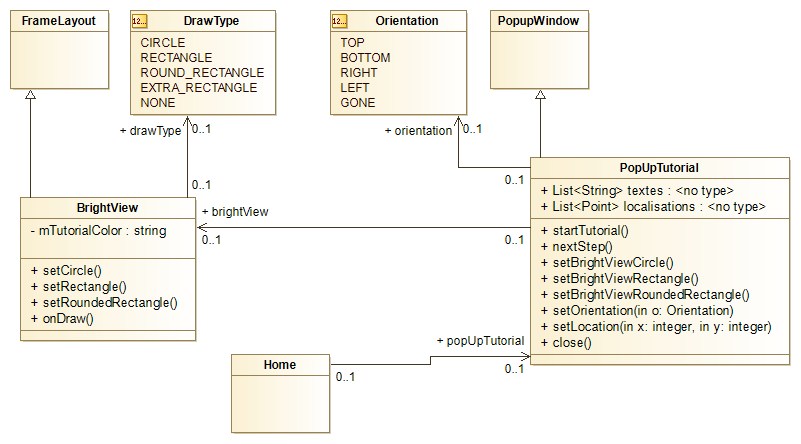
\includegraphics[width=115mm,scale=0.5]{images/diagramme.png}
  \caption{Diagramme UML simplifié du didacticiel}
  \label{fig:boat1}
\end{figure}

Le diagramme est volontairement simplifié pour faire apparaître l'essentiel sur la structure qui a été définie tout au long de cette partie. Home correspond au contrôleur de la page d'accueil où est appelé PopUpTutorial. Il n'est pas nécessaire de connaître les valeurs passées aux fonctions dans la plupart des cas, l'important ici est juste de comprendre la structure globale du didacticiel.

Une fois tout ceci mis en place on peut dorénavant dérouler un tutoriel avec les différentes étapes. Dans la version qui a été définie par Tastycloud le didacticiel comportait 9 étapes (ou 8 selon les cas de restaurants). Ces étapes sont disponibles en annexe. Ce qu'il faut savoir c'est que certaines de ces étapes nécessitent de simuler une navigation et donc de parcourir l'application. Pour un cas unique de restaurant on peut facilement définir un chemin (et c'est d'ailleurs ce qui a été fait dans un premier temps). Cependant, comme dit précédemment, chaque restaurant a ses spécificités. Par exemple certains restaurants ne possèdent pas les allergènes, certains n'ont pas les même structure dans le menu de gauche. Il faut donc adapter tout ceci pour que le didacticiel couvre le plus de cas possible. Un exemple a été pour l'étape où l'on présente la page de sélection de produits. Dans certains cas le menu est différent. 

\begin{figure}[!htb]
  \centering
  \begin{minipage}[b]{0.45\textwidth}
    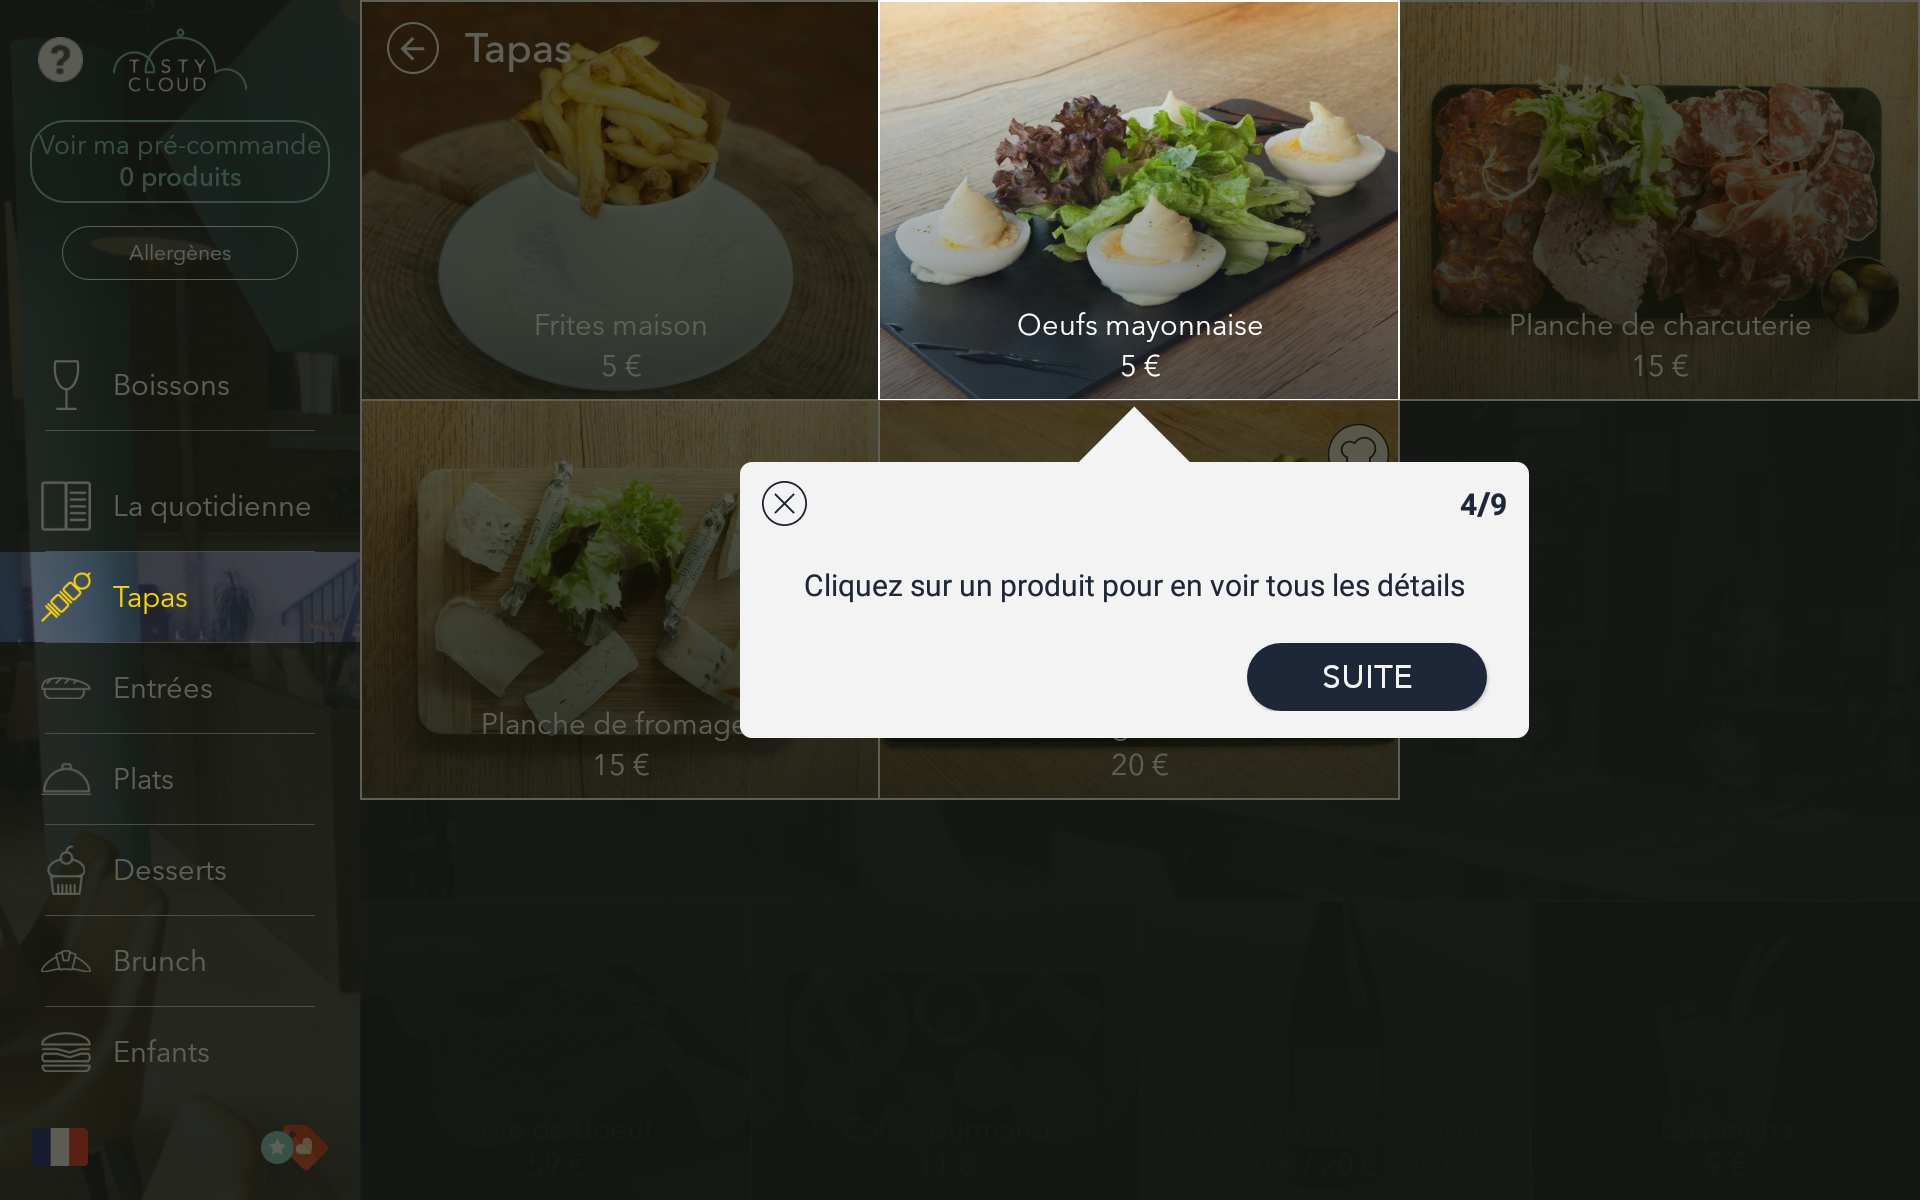
\includegraphics[width=\textwidth]{images/tutoriel_screen2.png}
    \caption{Étape 4 du didacticiel}
  \end{minipage}
  \hfill
  \begin{minipage}[b]{0.45\textwidth}
    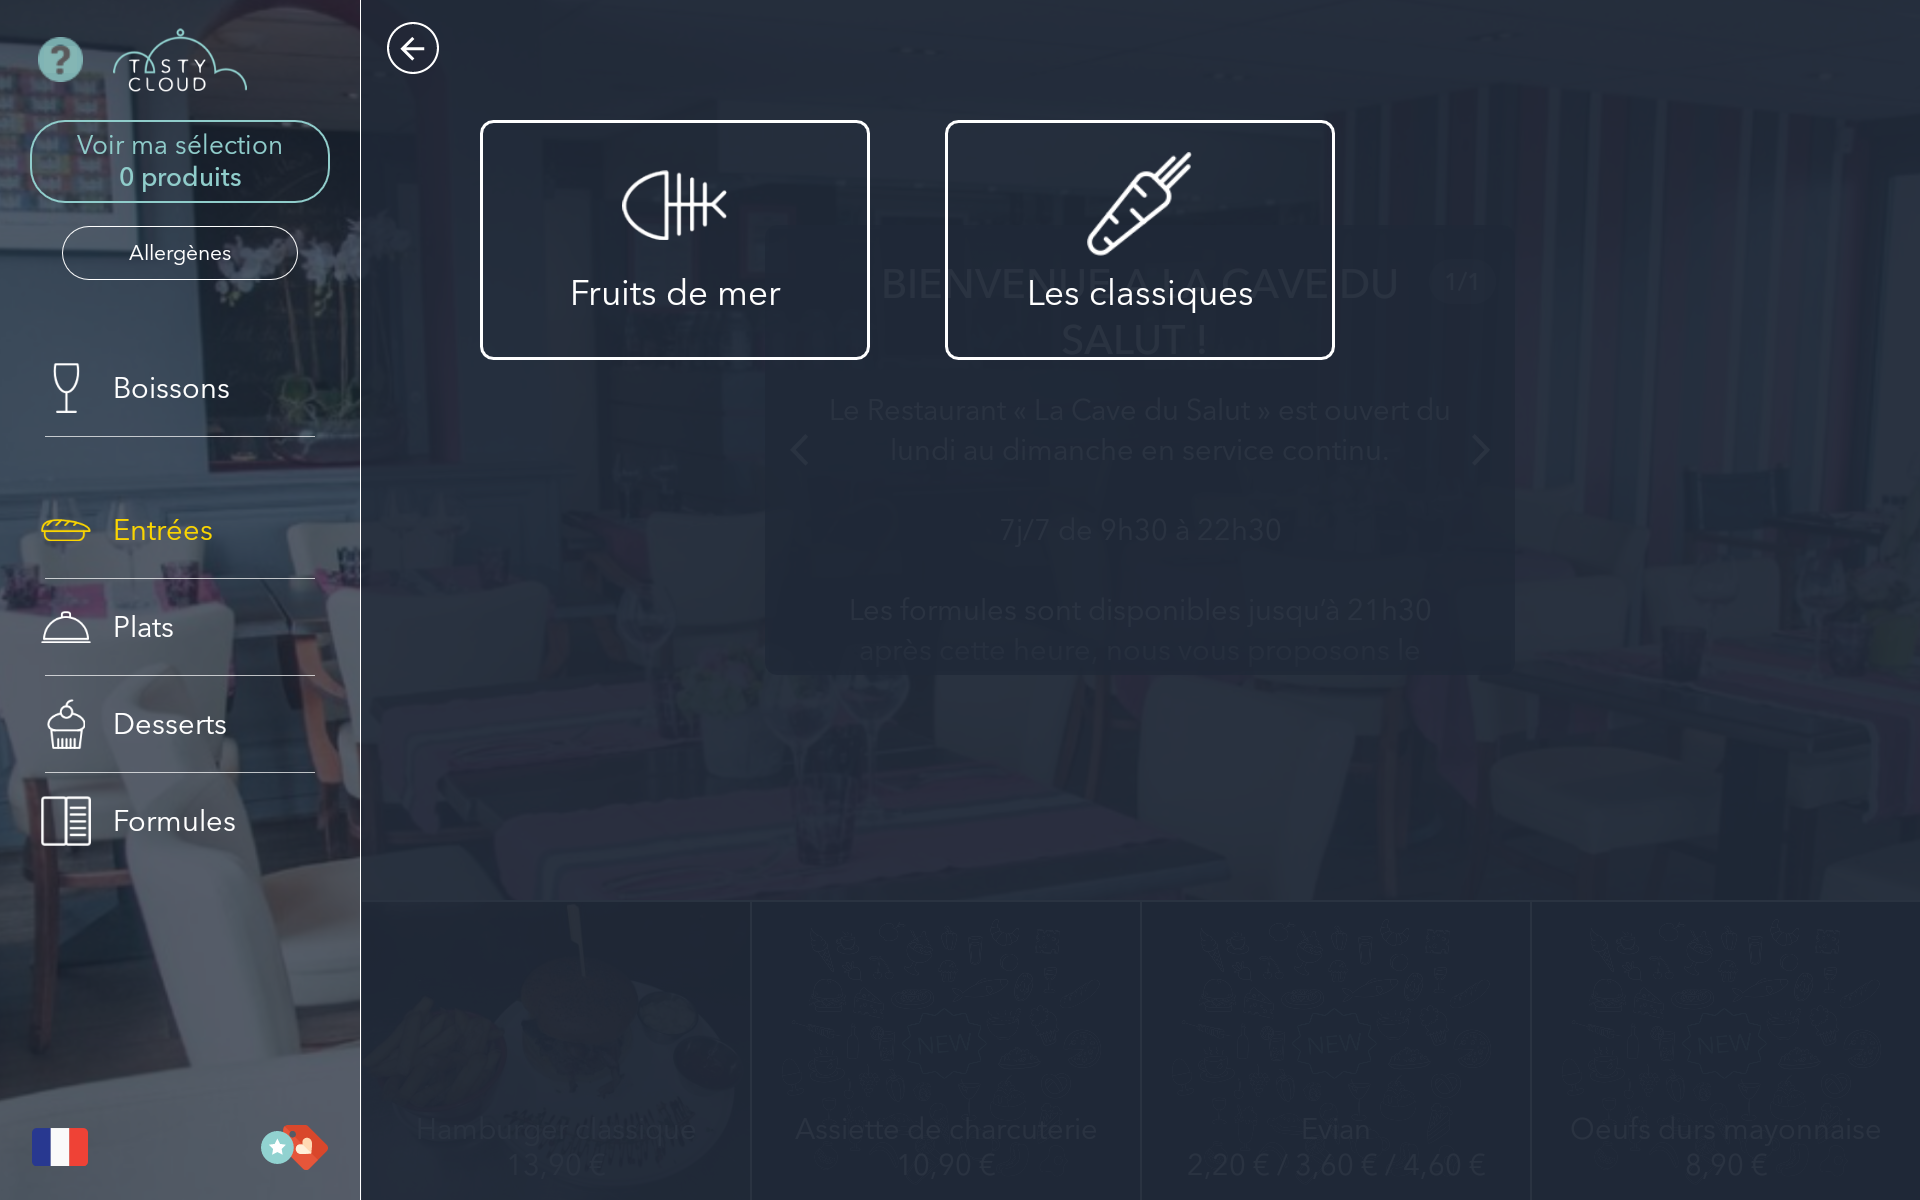
\includegraphics[width=\textwidth]{images/tutoriel_screen1.png}
    \caption{Menu entrées}
  \end{minipage}
\end{figure}

Comme on peut le voir sur les captures d'écrans, il y a parfois un autre menu avant d'atteindre la sélection des produits. Il a fallu, dans le code vérifier ce cas et l'ignorer pour contourner ce problème. Il faut aussi gérer la présence ou non des allergènes. Heureusement le restaurant courant et ses options peuvent être récupérés depuis le home et ces cas particuliers peuvent être traité plus facilement.

Un autre problème a été que le tutoriel nous montre aussi comment commander et comment voir sa sélection. Il a donc fallu simuler un choix et l'afficher dans l'onglet des commandes. Seulement, lorsque l'on mémorise un choix dans l'application celui-ci est envoyé à la base de données. Or, logiquement dans notre cas le didacticiel est juste là pour montrer le fonctionnement de l'application et non pas pour faire des appels à la base. Pour faire face à ce problème j'ai décidé de créer une variable associée au restaurant qui est disponible dans les classes de sélection de l'application et qui permet de faire un test (donc avec cette variable qui est un booléen) pour savoir si oui ou non il faut faire un appel à la base. Dans un premier temps, il n'était même pas prévu de simuler l'utilisation de l'application avec un produit mais finalement lors du développement du tutoriel nous avons trouvé cela plus logique. 

Par exemple, dans la capture d'écran que l'on a sur la page suivante, "les frites maison" sont ajoutées dans la sélection mais elles ne le sont pas dans la base données. C'est à dire qu'elles sont ajoutées seulement graphiquement sur l'application. Dans le cas où l'utilisateur quitte le tutoriel à cette étape, l'élément ajouté "virtuellement" dans la sélection est supprimé. Et seulement celui-là si l'utilisateur avait déjà choisi des produits avant de lancer le tutoriel. Rajoutons aussi que lorsque l'on appui sur le bouton quitter l'application revient toujours sur le menu home, et si on clic sur le didacticiel dans un sous menu, le tutoriel commencera toujours aussi sur le home (sinon le parcours ne se ferait pas sur les bonnes pages de l'application).

\clearpage

\begin{figure}[!htb]
  \centering
  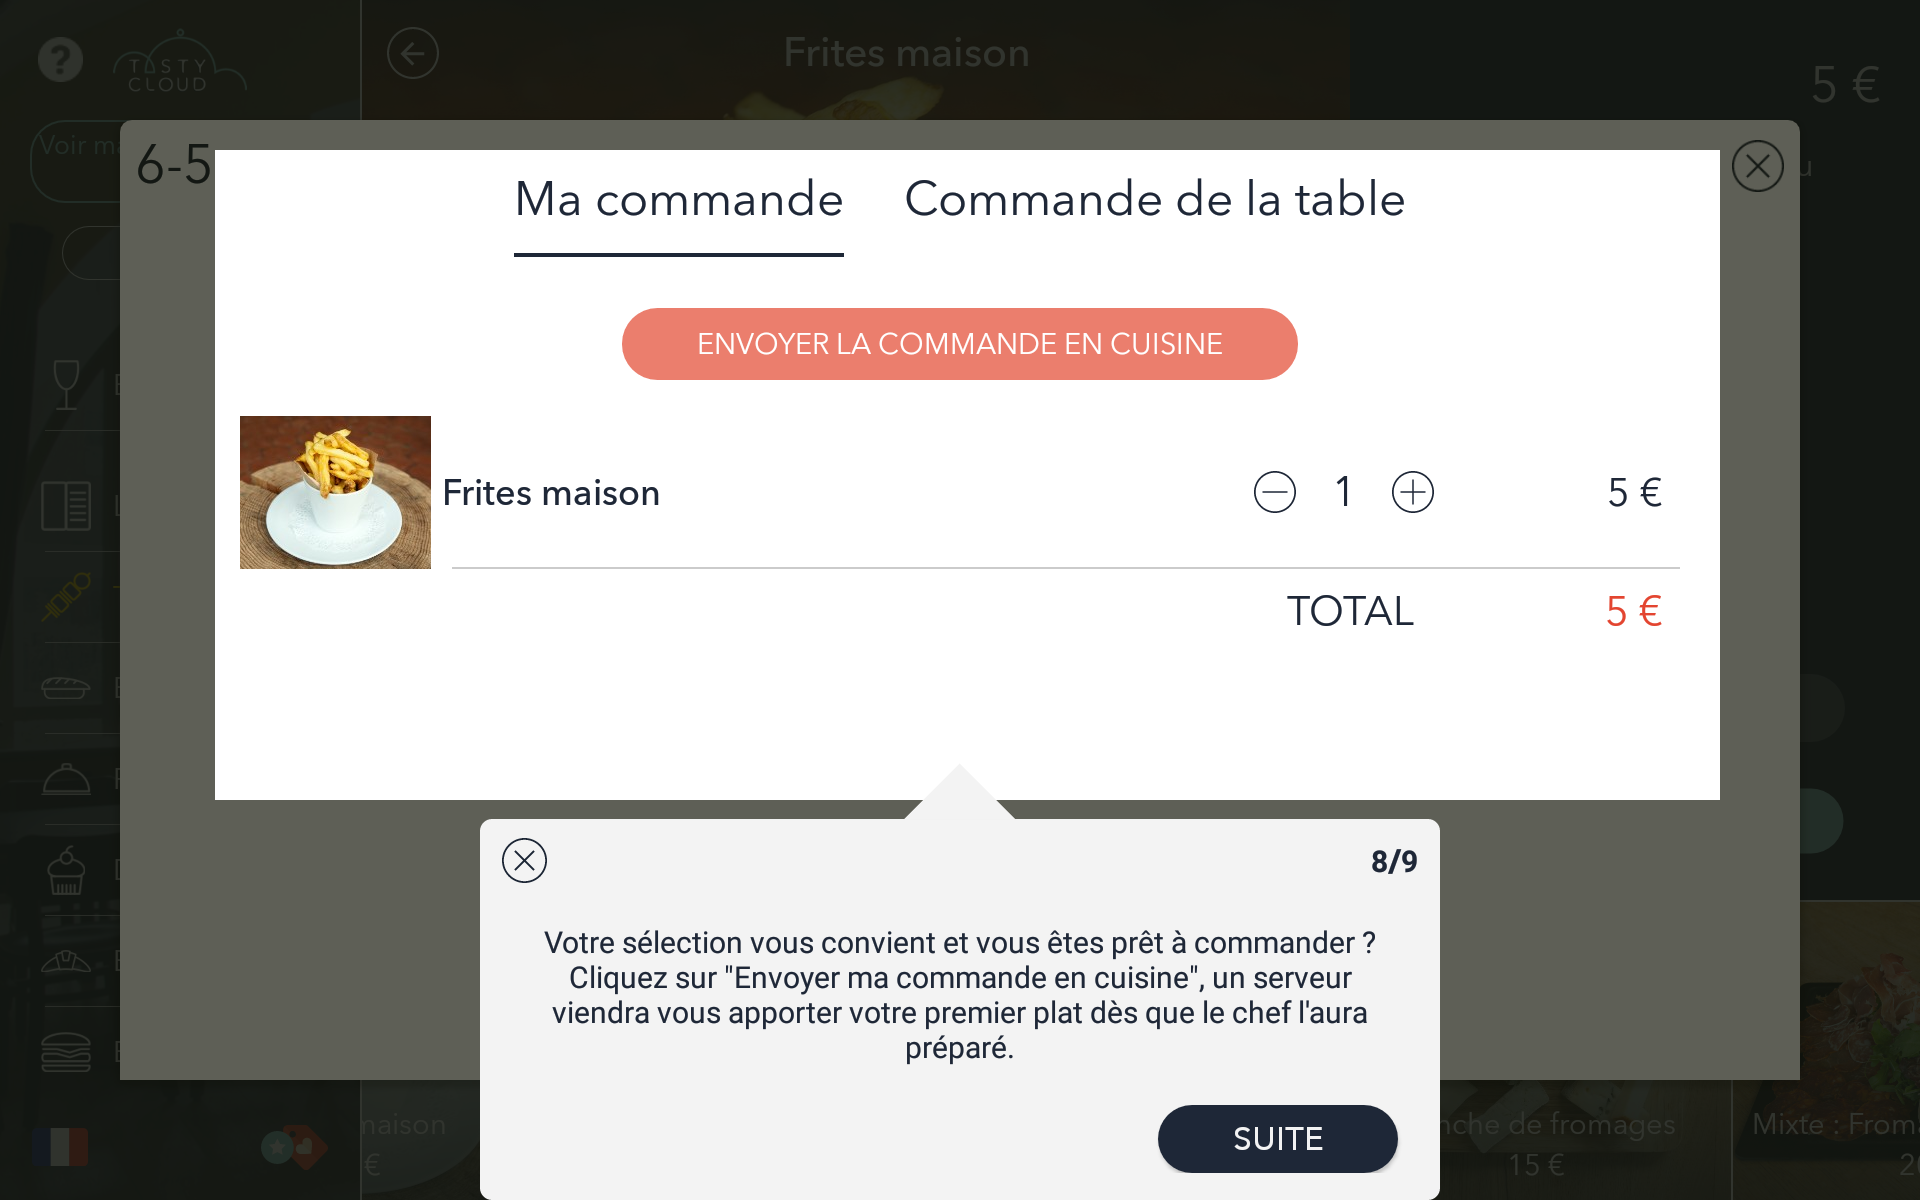
\includegraphics[width=115mm,scale=0.5]{images/tutoriel_screen3.png}
  \caption{Étape de présentation de la commande}
  \label{fig:boat1}
\end{figure}

Une fois tout ceci mis en place ainsi que la charte graphique, il a fallu gérer les textes des pop-ups. Plus particulièrement les traductions. Déjà auparavant j'avais dès le début de la conception du didacticiel prévu le fait que la taille des pop-ups s'adapterait à la taille du texte pour les traductions. Cependant, il fallait préparer le code pour que selon la langue choisie le didacticiel s'adapte à cette langue. Dans un premier temps, tous les textes étaient définis en "dur" dans le code, il a fallu faire un appel vers la base de données pour récupérer les traductions. Dans le code on fait un appel au presenter du home et l'on définit les clés qui seront récupérées dans le code. Pour les textes à écrire tout est défini dans le back office de l'application.

\begin{figure}[!htb]
  \centering
  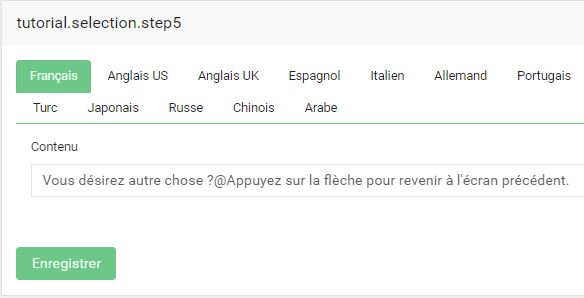
\includegraphics[width=115mm,scale=0.5]{images/tutoriel_trad.JPG}
  \caption{Clé de traduction}
  \label{fig:boat1}
\end{figure}

Voici un exemple de clé de traduction, on va dans les onglets pouvoir choisir d'autres langues. Pour finir j'ai mis en place le mot clé "@" pour pouvoir faire des retours à la ligne dans le cas où l'on doit adapter le texte. C'est ainsi que s'achève ma mission sur le didacticiel qui a été très intéressante d'un point de vue conception et modélisation. Le didacticiel a ensuite été ajouté à la version suivante de l'application et a pu être mis en place dans différents restaurants.

\subsection{Zone cliquable}

Plusieurs retours clients ont fait état de difficultés à bien enclencher le clic sur certains boutons de l'application. Certains boutons ont une forme rectangle arrondie alors que la zone cliquable est un rectangle simple. Par exemple si on clic sur les bords de ces boutons on ne pourra pas enclencher l'appel à la fonction qui écoute sur ce clic. Cela est d'autant plus problématique que ce problème est survenu lors de démonstrations à des clients. Pour pallier ce problème, il m'a été demandé d'agrandir cette zone cliquable sur certains boutons. Plus particulièrement sur les boutons du menu à gauche et sur le bouton pour commander un produit. C'est le genre de boutons constamment présentés en démonstration de la solution.

Pour pallier ce problème et éviter les risques, j'ai cherché une solution pour agrandir la zone cliquable et je suis notamment tombé sur "TouchDelegate", une classe d'assistance pour gérer la situation ou une vue doit avoir une surface tactile plus grande bien sûr dans les limites de la vue englobante ou père. Avec cette classe, j'ai pu notamment définir sur une vue avec sa vue parente une zone cliquable plus grande. Il suffit pour cela de récupérer les coordonnées de la vue (par exemple le bouton allergène) puis de lui affecter des valeurs plus grande de X dp (density-independant pixel) pour chacun des quatre points du rectangle (top, left, bottom right). Pour finir, les vues ont un attribut "touchelegate" et il suffit alors de leur affecter le touchDelegate créé.

Seulement comme dit précédemment, TouchDelegate ne marche que pour une vue. Or, dans de nombreux cas j'ai besoin d'agrandir la zone cliquable sur plusieurs boutons du même layout. Par conséquent il a fallu que je redéfinisse la fonction "onTouchEvent" pour que cette dernière puisse appeler tous les "onTouchEvent" d'une liste de touchDelegate.
Pour faire face à ce problème j'ai décidé d'appliquer le design pattern Composite, j'ai ainsi défini une classe TouchDelegateComposite à laquelle on peut ajouter ou supprimer des TouchDelegate. Cette classe a donc en attribut une liste de TouchDelegate, la redéfinition de onTouchEvent et enfin la fonction pour faire le rectangle agrandi.

\begin{figure}[!htb]
  \centering
  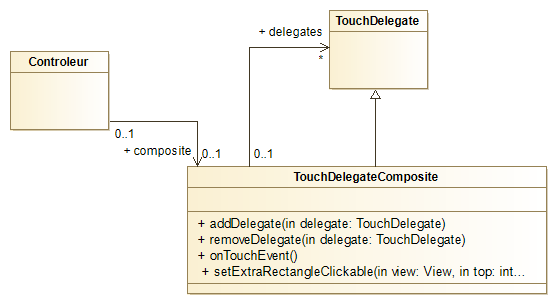
\includegraphics[width=115mm,scale=0.5]{images/diagramme_composite.png}
  \caption{Diagramme UML du composite}
  \label{fig:boat1}
\end{figure}

Dans un souci de réutilisabilité, j'ai voulu créer une fonction qui va s'occuper de tout ; l'ajout dans la liste de délégation, la récupération du rectangle et la création du rectangle agrandi. Elle fera aussi l'affectation du delegate au père de la vue. Ainsi l'utilisateur n'aura qu'à utiliser le "setExtraRectangleClickable" (dont le code est disponible en annexe).

\clearpage

Voici, ainsi, comment du côté utilisateur on utilise un TouchDelegateComposite pour pouvoir l'utiliser sur plusieurs vues. Comme on peut le voir dans le diagramme, le TouchDelegateComposite peut être utilisé dans un contrôleur lors de la création de la page dans le OnAttach.

\begin{lstlisting}[frame=single]  % Start your code-block
    
var composite = TouchDelegateComposite(Rect(), homeRelative)

composite.setExtraRectangleClickable(selectionLayout, 10, 20, 5, 20)
composite.setExtraRectangleClickable(allergensTextView, 5, 30, 20, 20)
composite.setExtraRectangleClickable(aproposView, 25, 25, 25, 25)
composite.setExtraRectangleClickable(mTutorial, 15, 20, 5, 12)
    
\end{lstlisting}

Comme on peut le voir c'est aujourd'hui très simple d'utilisation. Si il faut plus tard dans l'application refaire ce système de zone tactile agrandie il suffira alors d'initialiser un composite en lui passant un rectangle et une vue (qui ne sert qu'à récupérer le contexte de l'application). Ensuite, on appellera la fonction avec la vue à laquelle on veut agrandir la zone tactile et les valeurs en dp à agrandir (haut, gauche, bas et droite). Dans l'exemple de code ci-dessus on peut par exemple voir que cela a été fait sur le bouton de sélection (selectionLayout), allergènes, à propos et le bouton de tutoriel.

\begin{figure}[!htb]
  \centering
  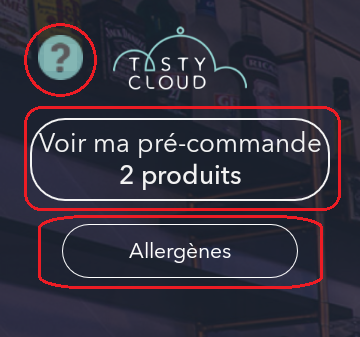
\includegraphics[width=115mm,scale=0.5]{images/tutoriel_click.png}
  \caption{Zones cliquables agrandies}
  \label{fig:boat1}
\end{figure}

Voilà pour se donner une idée ce que donne la zone tactile (en rouge pour chaque bouton) dans l'ajout du code ci-dessus. Alors qu'avant les bords des boutons en rectangle arrondi ne déclenchaient pas le clic, maintenant même si nous appuyons un peu à côté cela marche tout de même et par conséquent les problèmes qu'a pu rencontrer auparavant l'équipe lors de démonstrations n'ont plus lieu d'être.

\clearpage




%%% Local Variables: 
%%% mode: latex
%%% TeX-master: "isae-report-template"
%%% End: 
\section{Autres missions}
\subsection{Option changement de couleurs des boutons}

Un autre retour client par rapport au bouton de commande révélait que ce dernier n'était pas assez visible pour l'utilisateur et que parfois il pouvait l'omettre. Bien évidemment, ce bouton est primordial dans l'application et il est important qu'il soit bien visible et bien utilisé. Avant cette mission, le bouton avait cette forme :

\begin{figure}[!htb]
  \centering
  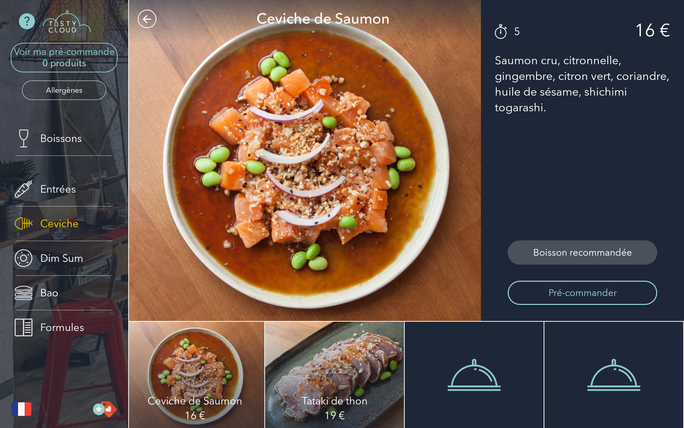
\includegraphics[width=110mm,scale=0.5]{images/couleur_bouton.png}
  \caption{Précédente version graphique}
  \label{fig:boat1}
\end{figure}

On parle ici du bouton "pré-commander" (Figure 3.16), ce dernier présentait auparavant une animation qui le mettait en avant mais celle-ci a dû être retirée. Après concertation sur le basecamp nous avons fait différents choix de couleur qui ont put être discutés en interne avec l'équipe. De toutes ces couleurs je me suis chargé d'en faire des captures d'écran et de les partager. Nous nous sommes concertés sur 2 choix de couleurs précis, le blanc et bleu plein.

\begin{figure}[!htb]
  \centering
  \begin{minipage}[b]{0.45\textwidth}
    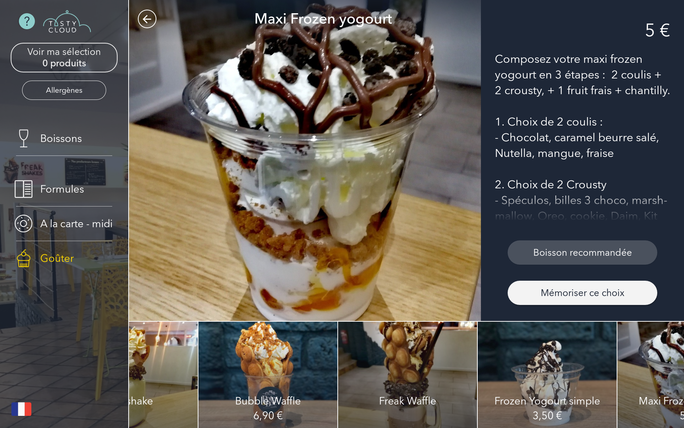
\includegraphics[width=\textwidth]{images/couleur_bouton2.png}
    \caption{Couleur blanche retenu}
  \end{minipage}
  \hfill
  \begin{minipage}[b]{0.45\textwidth}
    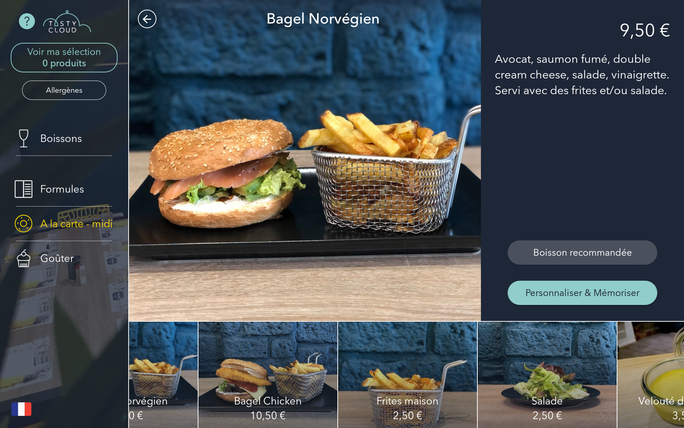
\includegraphics[width=\textwidth]{images/couleur_bouton3.png}
    \caption{Couleur bleu retenu}
  \end{minipage}
\end{figure}

On observe que ce changement affecte aussi le bouton de sélection (voir sa sélection) dans le cas de la couleur blanche. En effet ce dernier a alors des contours blancs. Le problème de cette solution est que l'on a alors 2 couleurs. On a donc décidé de laisser le choix à l'utilisateur (donc ici le restaurateur) de choisir une de ces deux couleurs pour son restaurant. Ce choix s'officie dans le back office où la couleur bleu avec le fond plein est présente par défaut et où la couleur blanche peut être choisie.

Le restaurateur dispose en effet de différentes options cochables ou non comme on peut le voir depuis cette capture d'écran du back office :

\begin{figure}[!htb]
  \centering
  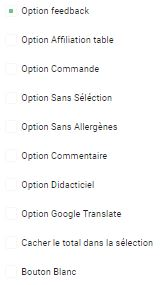
\includegraphics[width=40mm,scale=0.5]{options_backoffice.JPG}
  \caption{Options du back office}
  \label{fig:boat1}
\end{figure}

Pour que cette option fonctionne il a donc fallu rajouter une ligne dans la table "Restaurant" et mettre cela à jour dans les entités dans le code. Avec l'aide de mon tuteur qui avait déjà réalisé des ajouts de fonctionnalités similaires, j'ai pu savoir rapidement les changements à effectuer dans le code. Changer donc l'entité, le modèle (la classe) et le JSON. Tout ceci va nous permettre de faire le lien avec le back office. Il suffit à chaque fois d'ajouter une ligne pour le cas du bouton blanc. 

Une fois ceci terminé on peut récupérer directement avec le restaurant courant la valeur de ce booléen. Il ne faudra alors plus que chercher où mettre cette couleur. En effet elle peut s'appliquer aussi lorsque l'application recommande des plats ou bien lorsque l'on choisit une formule. Une fois tous les cas énumérés ajoutés nous avons pu intégrer cette fonctionnalité dans la version suivante de l'application.

\begin{figure}[!htb]
  \centering
  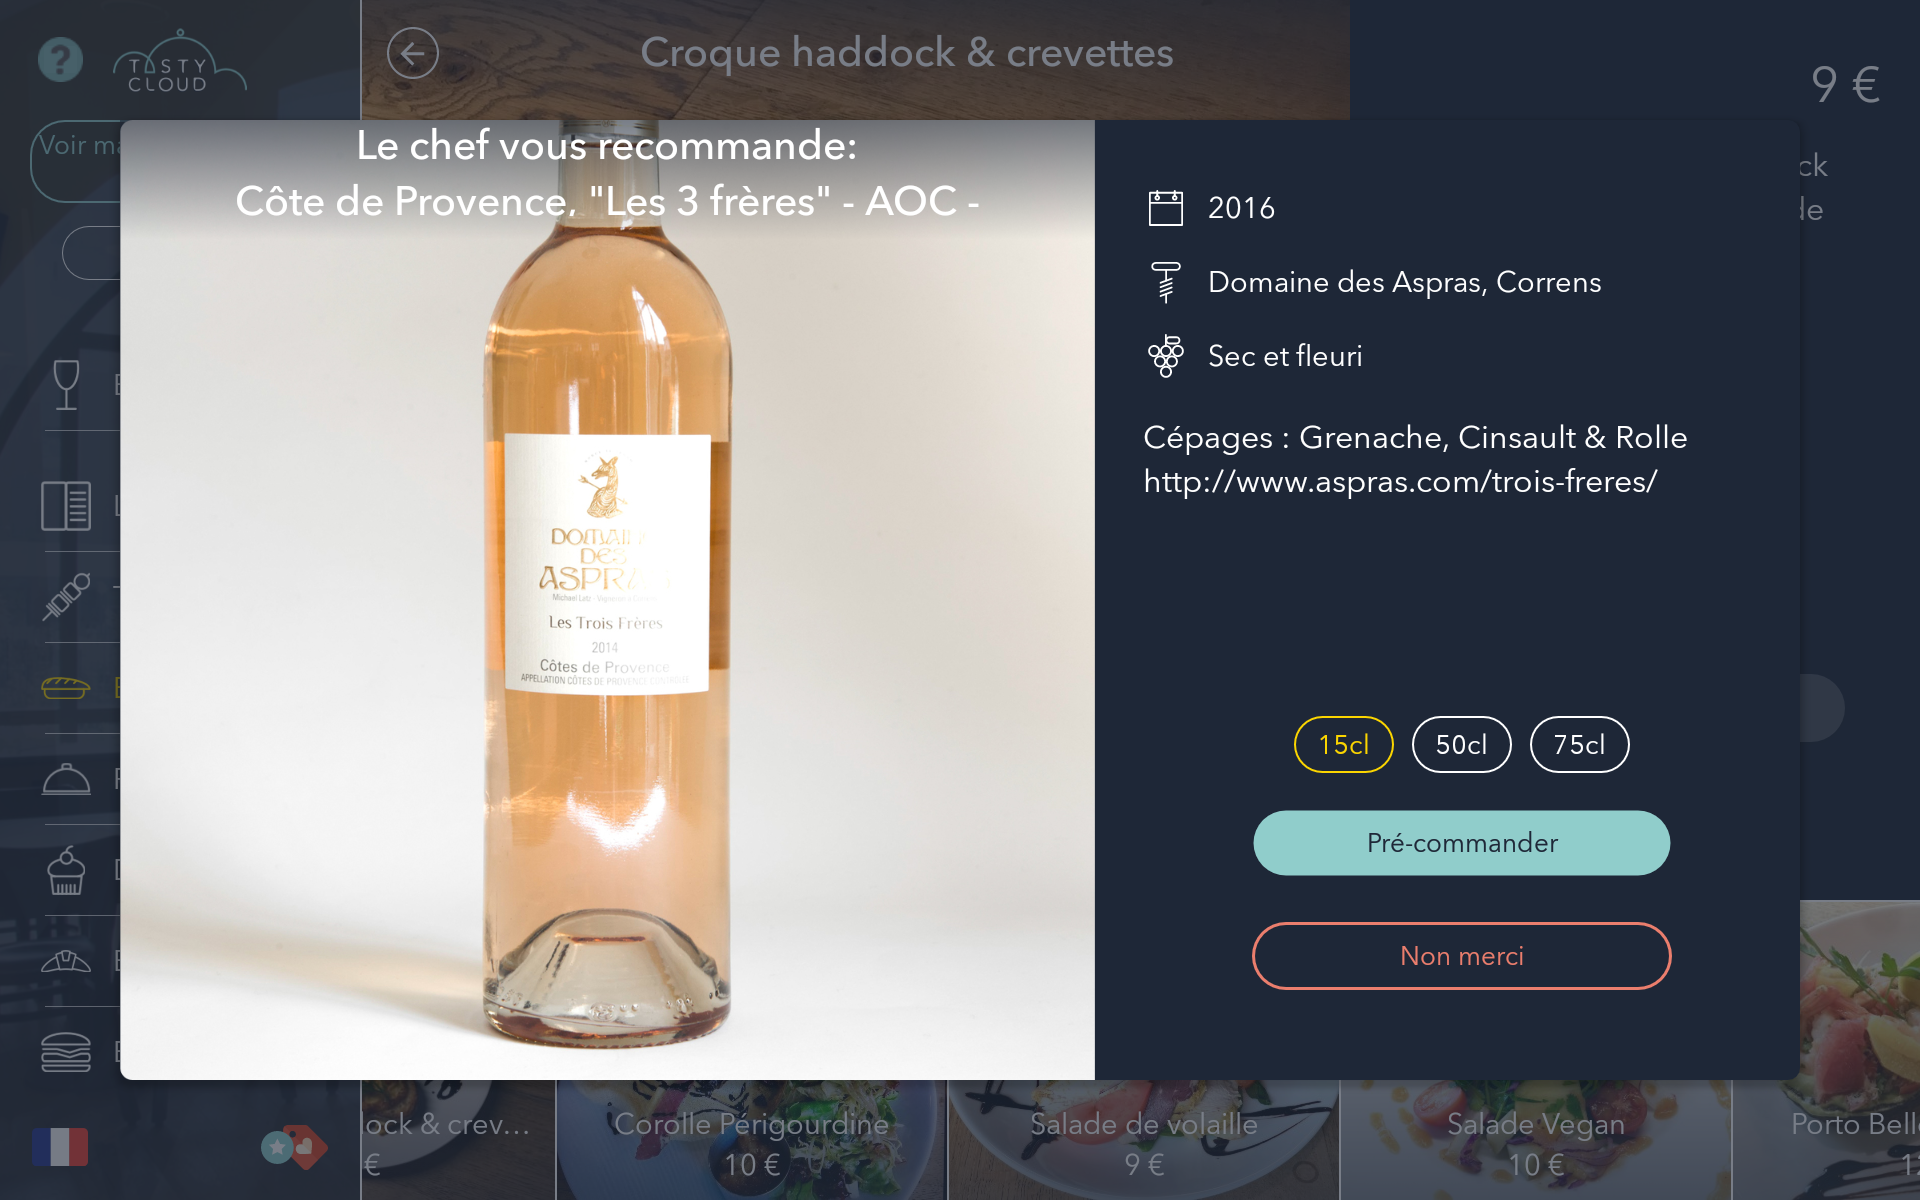
\includegraphics[width=110mm,scale=0.5]{images/couleur_bouton4.png}
  \caption{Une pop-up de recommandation}
  \label{fig:boat1}
\end{figure}

\subsection{Sélection dynamique}

\begin{figure}[!htb]
  \centering
  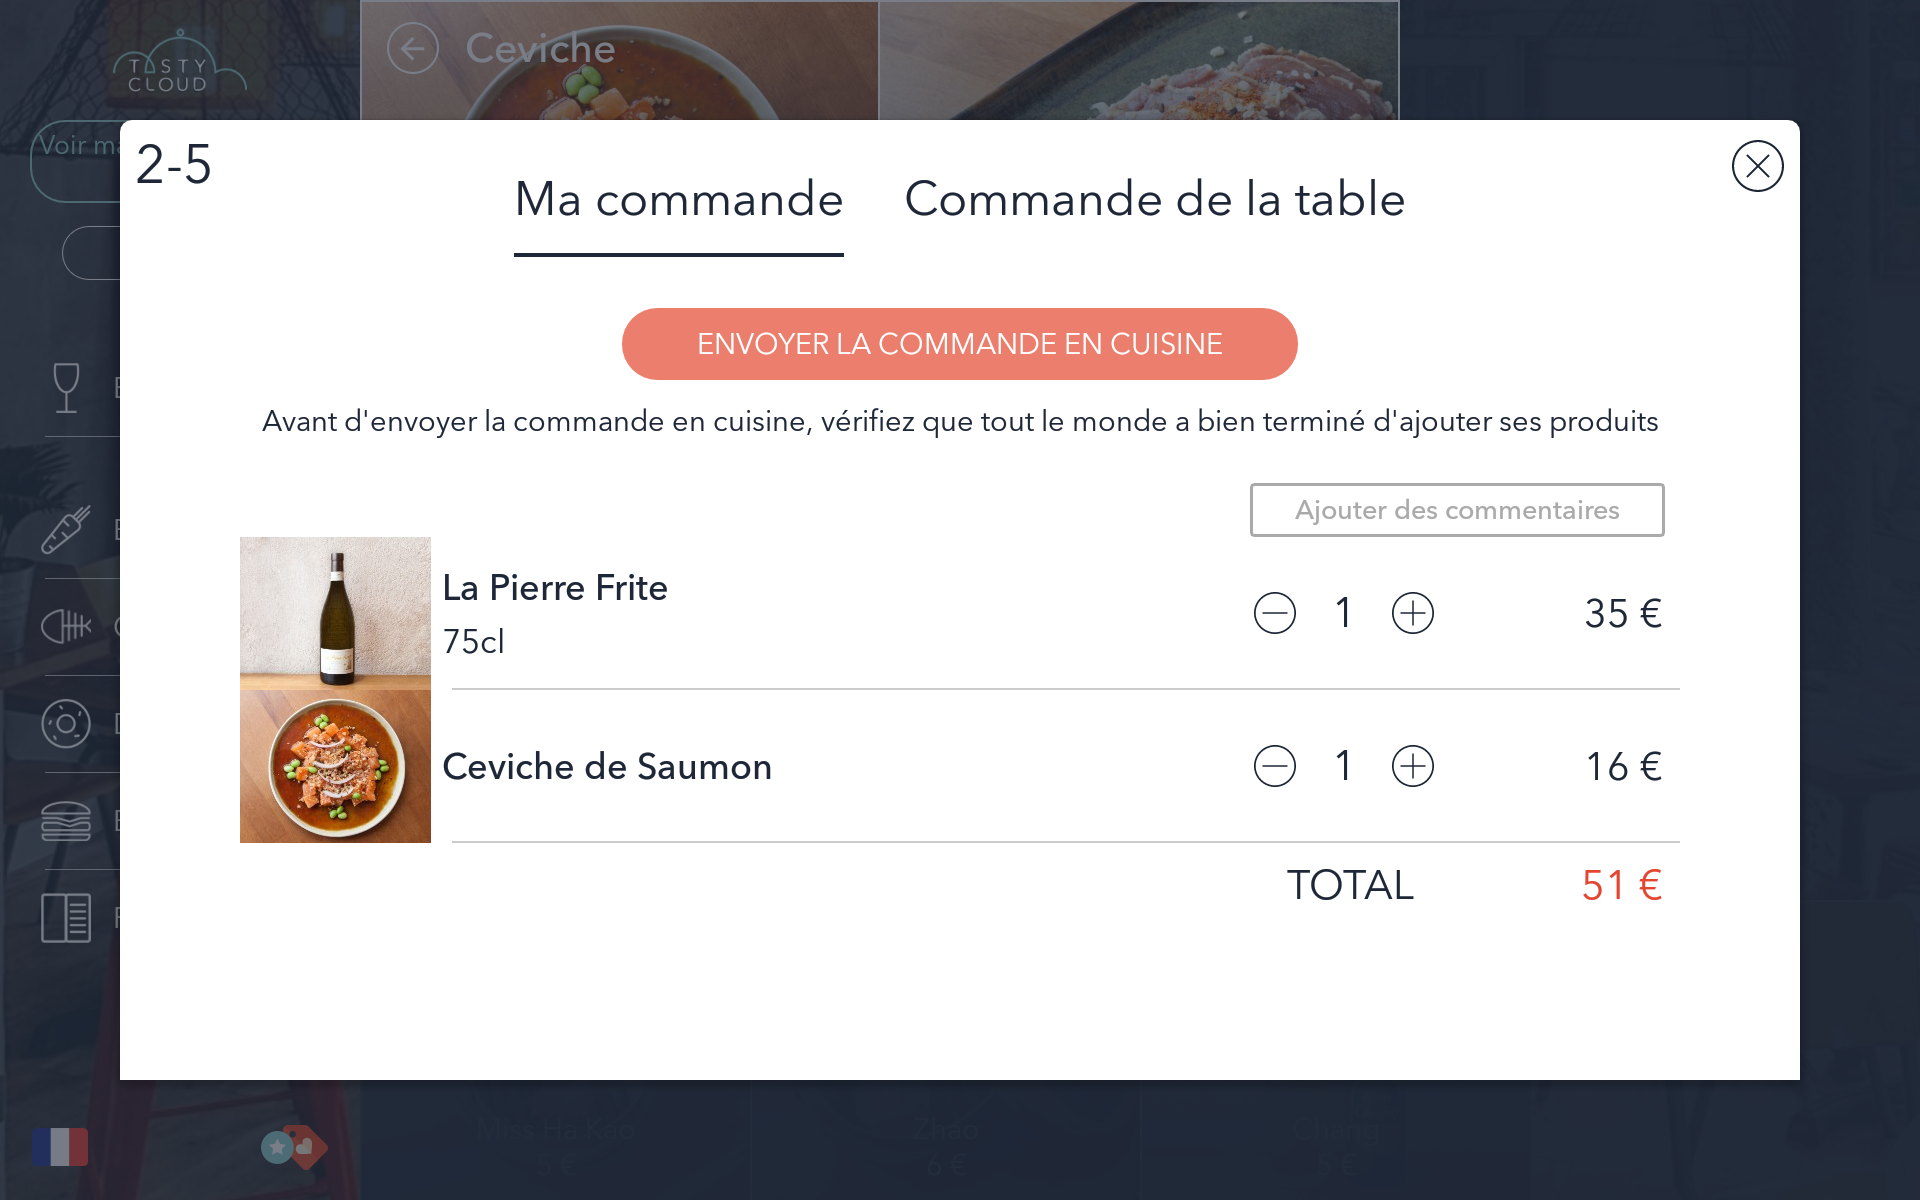
\includegraphics[width=115mm,scale=0.5]{images/selection.png}
  \caption{Menu de sélection}
  \label{fig:boat1}
\end{figure}

Voici le menu de sélection de l'application. Pour certains restaurants, ce menu propose la commande comme dans le cas de la capture d'écran. Il peut aussi être proposé plusieurs tablettes pour une table ce qui fait qu'un utilisateur peut commander sur sa tablette, voir ce qu'il a commandé et aussi voir ce qui a été commandé sur la table dans l'onglet "Commande de la table". L'idée de la mission sur la sélection dynamique est que cet onglet apparaît si et seulement si quelqu'un d'autre a commandé quelque chose. On peut donc aussi avoir le cas ou "Ma commande" est vide et "Commande de la table" est présent. Tout dépend la manière dont les plats sont commandés. Le but de cette mission était aussi que tout cela se fasse en temps réel. Pour ce faire mon tuteur m'a expliqué que je devais passer par le presenter et faire cela de manière asynchrone comme ce qui a par exemple été fait pour l'affiliation. Dans le contrôleur j'ai donc une fonction de ce type :

\begin{lstlisting}[frame=single]  % Start your code-block
    
    override fun bindTablesEachOther(isDifferent: Boolean) {
        if(isDifferent)
            tab2.visible()
        else
            tab2.gone()
    }
    
\end{lstlisting}

Elle permet simplement de cacher oui ou non le deuxième onglet, si les deux listes sont différentes. Pour ce qui est du paramètre passer à la fonction, c'est via le presenter qu'il est appelé. On va récupérer les deux listes depuis la base de données et faire les tests nécessaires pour savoir si oui ou non elles sont différentes. J'ai, dans un premier temps, fait simplement un test sur la taille des deux listes et retourner vrai si différent. Cependant, les listes sont différentes si le nombre de choix pour un produit change. Par exemple, il est possible que l'on ait la même taille dans la liste (par exemple 2 sur la figure 3.21) mais que dans la commande de la table l'on ait 2 ceviche de saumon et 1 vin "La Pierre Frite". Les listes auront bien la même taille mais le nombre de produits réels sera 2 chez moi et 3 sur la commande de la table.

\clearpage

Pour résoudre ce problème il a fallu faire plus de test. Nous avons le test des tailles il faut aussi tester les items un par un dans un foreach. Pour chacun on test si le nombre d'éléments est différent (1 vin ? 2 vin ?) et on test si c'est bien les mêmes produits. Si dans les deux cas il y a une différence alors on retournera vrai. Après avoir implémenté cette solution j'ai pu tester avec deux tablettes en même temps sur une table. Cela semblait bien fonctionner mais j'ai ensuite remarqué que les produits n'étaient pas rangés de la même façon selon que l'on soit dans le premier ou deuxième onglet.

\begin{figure}[!htb]
  \centering
  \begin{minipage}[b]{0.45\textwidth}
    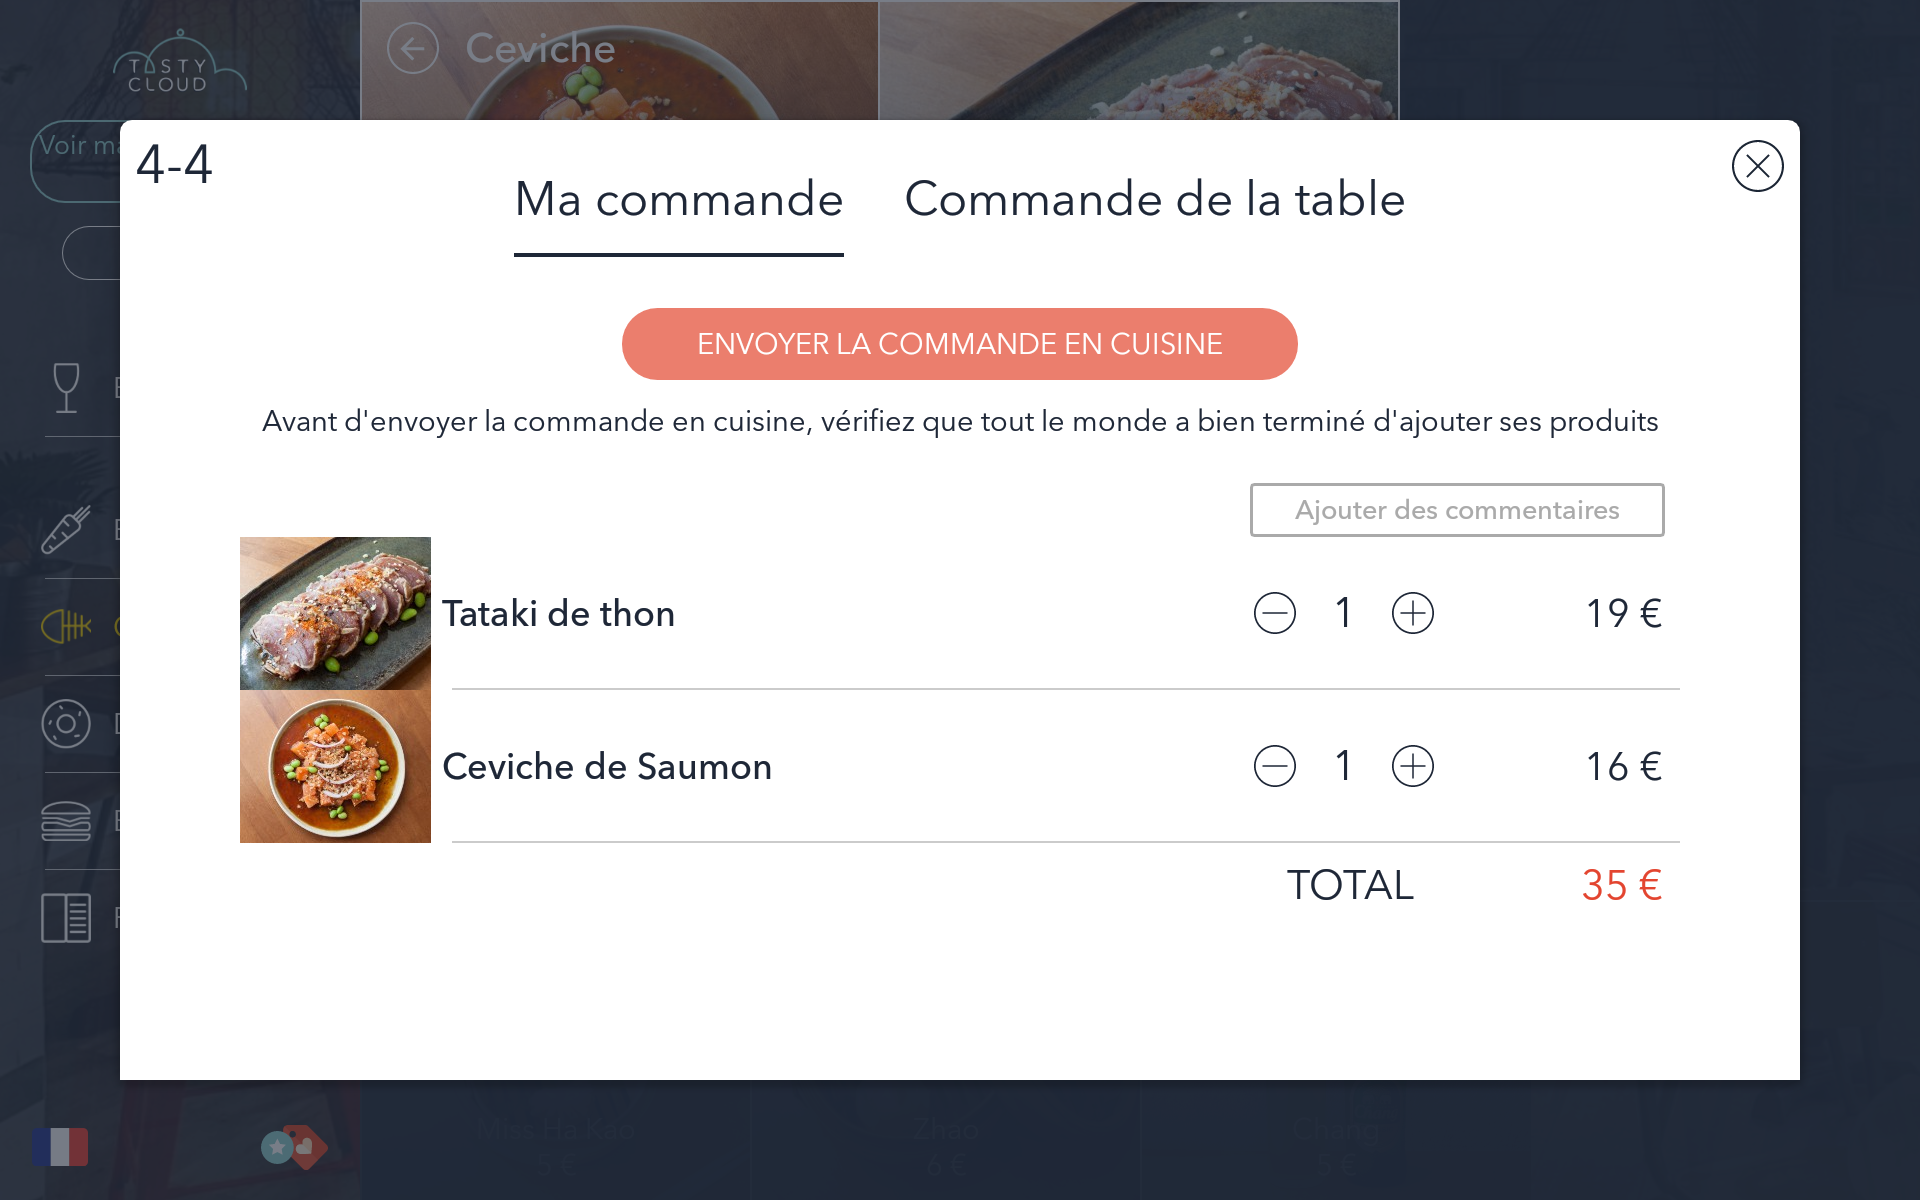
\includegraphics[width=\textwidth]{images/selection2.png}
    \caption{Onglet "Ma commande"}
  \end{minipage}
  \hfill
  \begin{minipage}[b]{0.45\textwidth}
    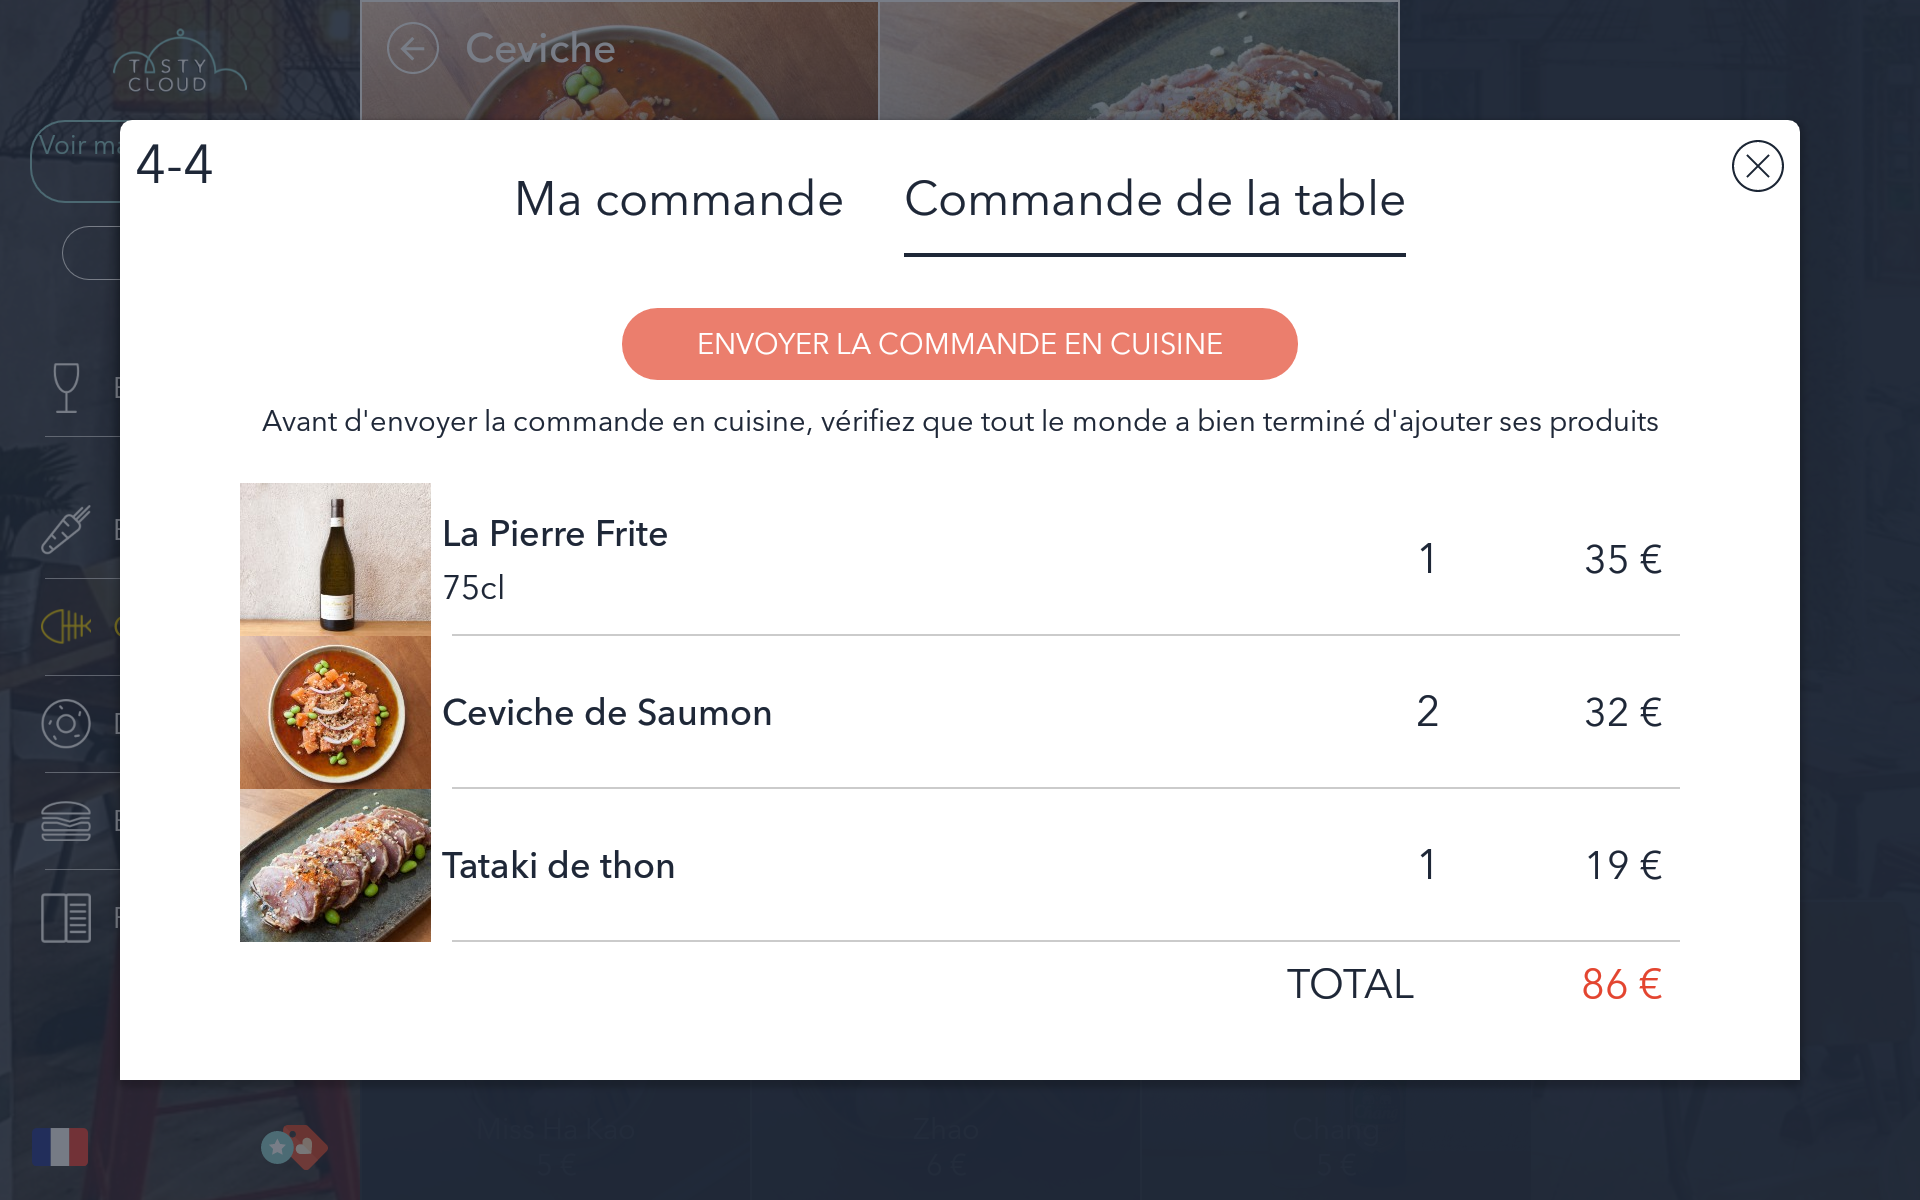
\includegraphics[width=\textwidth]{images/selection3.png}
    \caption{Onglet "Commande de la table"}
  \end{minipage}
\end{figure}

Par exemple dans ma commande, on a "Tataki de thon" puis "Ceviche de saumon" et ces deux aliments sont inversés dans commande de la table. Ceci s'explique que pour des raisons pratiques de traitements, les aliments dans commande de la table doivent être triés de façon précise (par les id des produits) et dans ma commande, ils doivent l'être dans l'ordre dans lesquels les produits ont été commandés. En conséquence de cela, il a fallu repenser le système de comparaison et c'est alors que j'ai décidé  de faire l'addition de tous les nombres de produits et de les comparer. Par exemple dans les deux captures d'écran ci-dessus, on aurait 2 à gauche et 4 à droite et donc l'affichage de l'onglet "Commande de la table".

Ainsi cette mission est pratique pour le visuel des clients en salle. Ils peuvent tout de suite connaître et voir en temps réel les ajouts et suppressions des convives avec lesquels ils sont. Lors de la visualisation de leur commande, ils peuvent voir si l'onglet "Commande de la table" apparaît ou non et ainsi constater si il y déjà eu une commande à leur table.

\begin{figure}[!htb]
  \centering
  \begin{minipage}[b]{0.45\textwidth}
    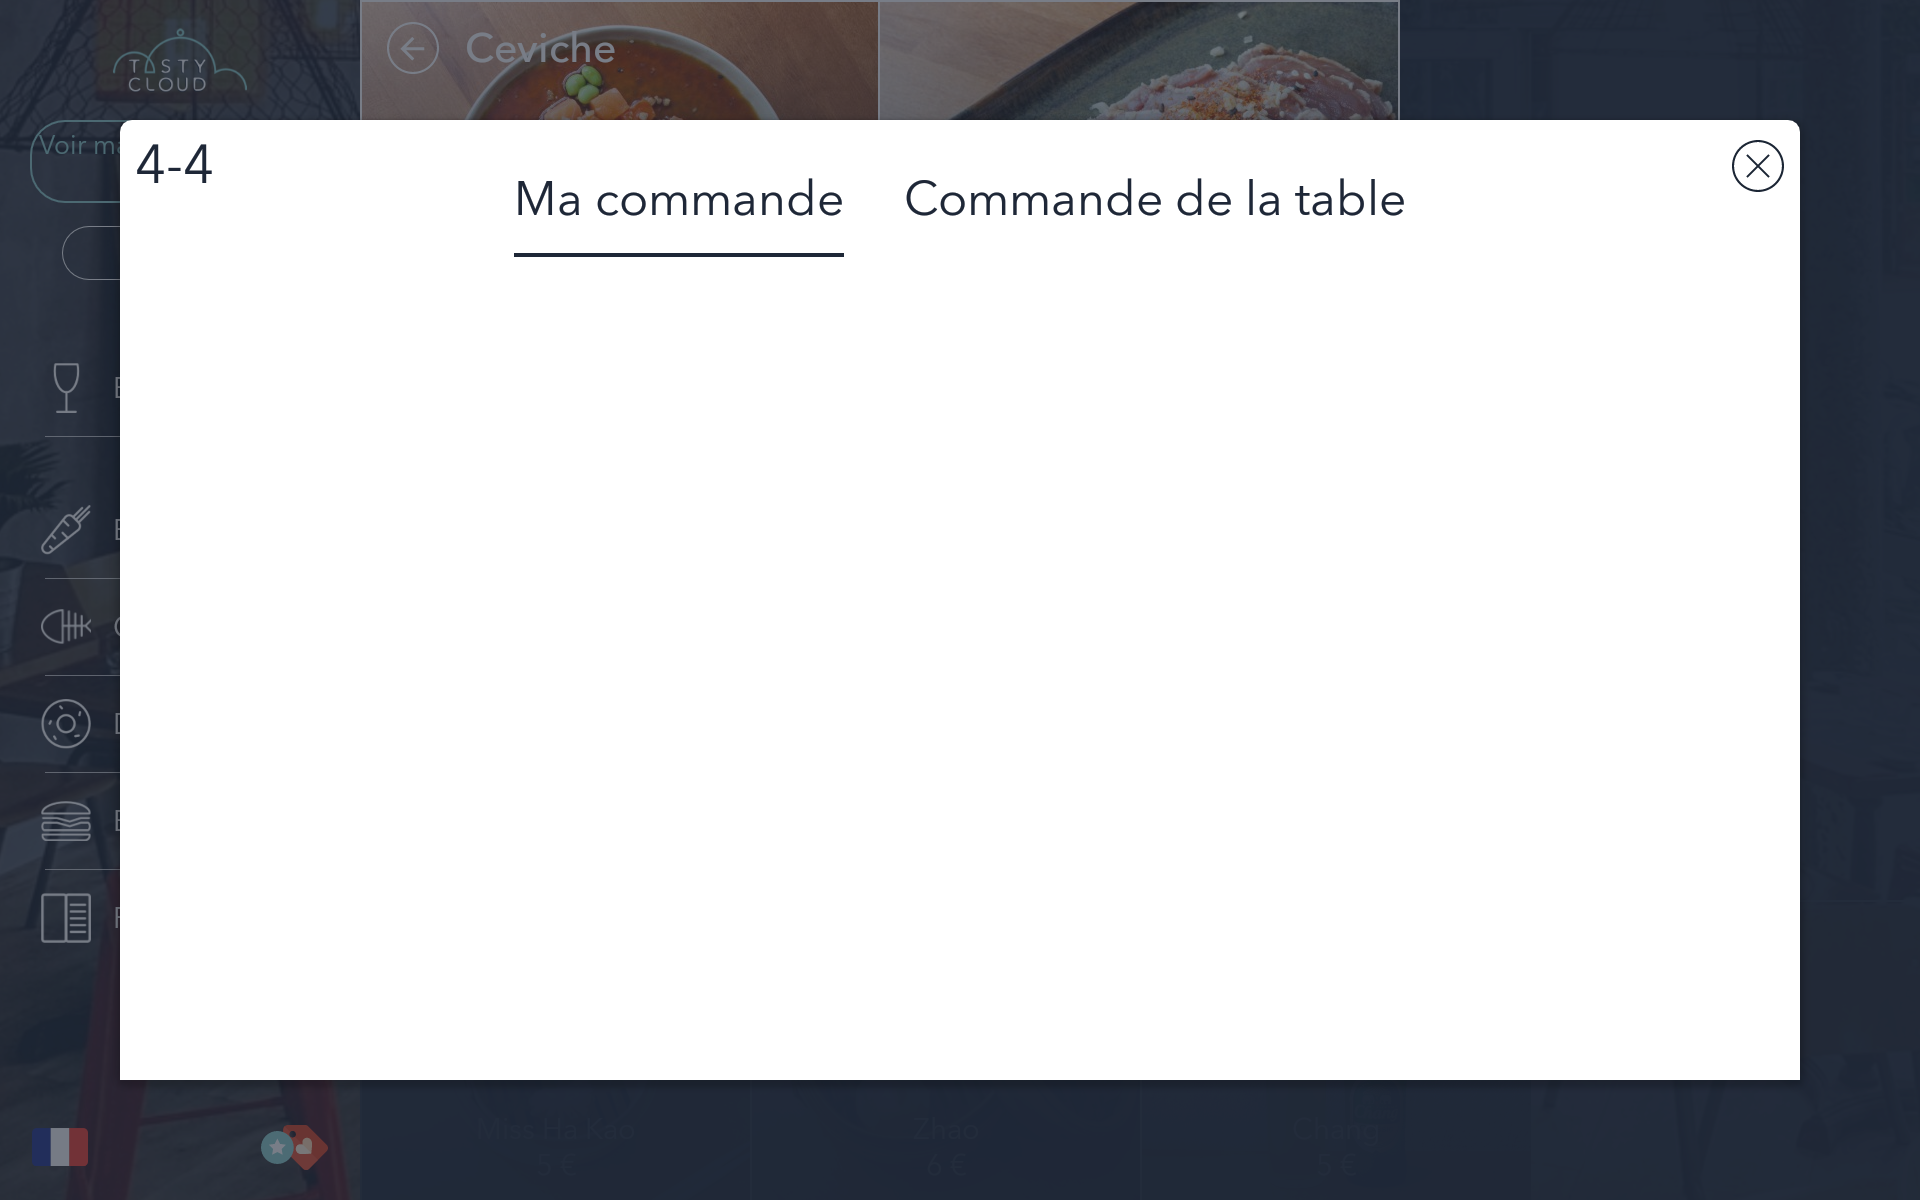
\includegraphics[width=\textwidth]{images/selection4.png}
    \caption{Cas ou quelqu'un a commandé}
  \end{minipage}
  \hfill
  \begin{minipage}[b]{0.45\textwidth}
    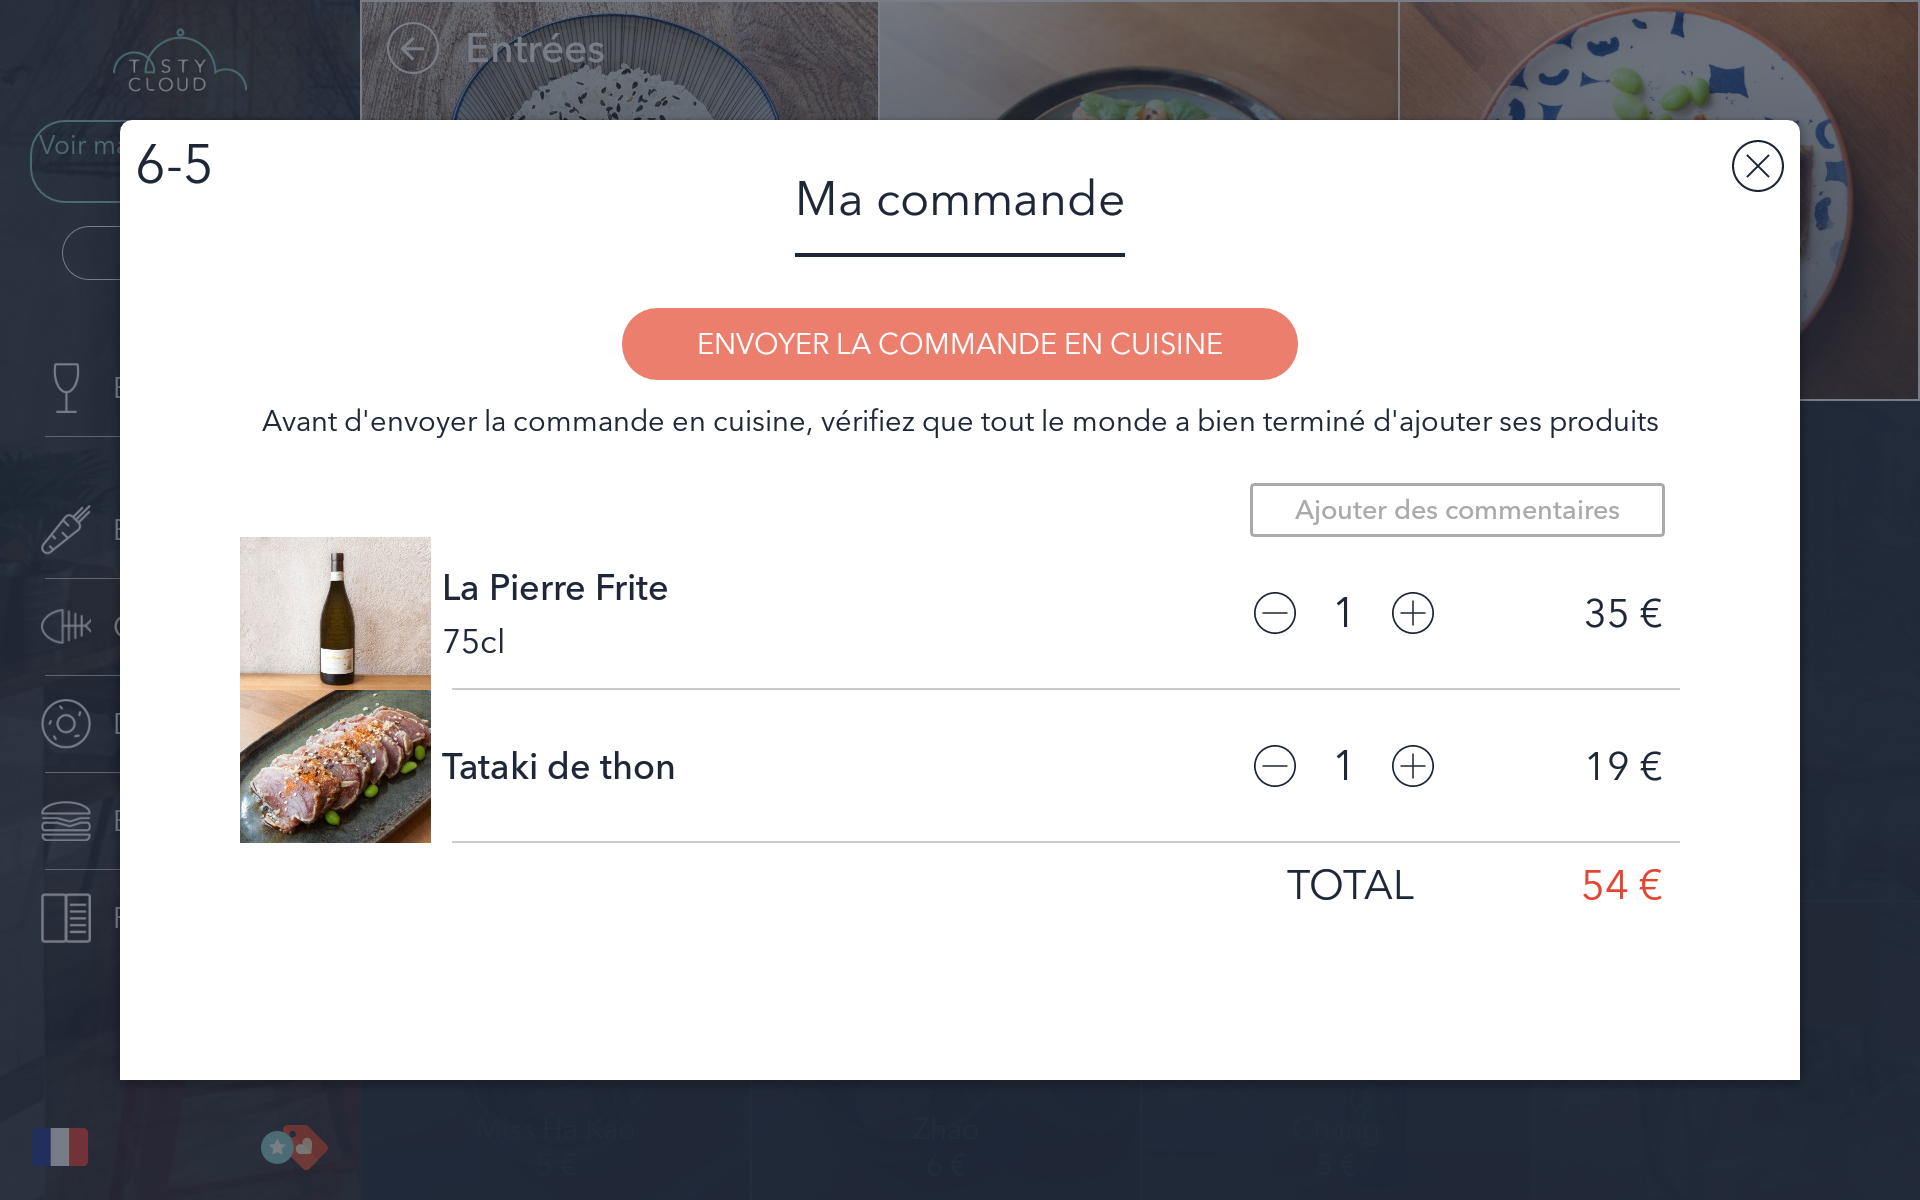
\includegraphics[width=\textwidth]{images/selection5.png}
    \caption{Cas ou je suis le seul à avoir commandé}
  \end{minipage}
\end{figure}



\subsection{Mot de passe pour la clôture de tables}

Certains serveurs mal informés appuyaient inopinément sur le bouton "Clôturer service". Ce bouton ferme toutes les tables du restaurant sans préavis. Avec mon tuteur, nous avons donc pensé à créer une boite de dialogue qui s'ouvre quand on appuie sur ce bouton. Cette dernière demande alors un mot de passe qui permet de clôturer toutes les tables et ainsi l'erreur n'est plus possible. Pour cette mission il n'y pas vraiment de modélisation ou de conception à réaliser. Seulement, nous nous sommes rendus compte que le DialogBox précédemment énoncé dans le rapport ne s'affichait pas sur la page d'affiliation. On a réutilisé alors PopupWindow qui lui se plaçait en premier plan sur l'affiliation (qui est aussi techniquement une pop-up). Il a alors fallu faire un XML correspondant à ce qui était requis pour la demande de clôture de tables soit un champ d'édition de texte pour le mot de passe et deux boutons "Valider" et "Fermer".

\begin{figure}[!htb]
  \centering
  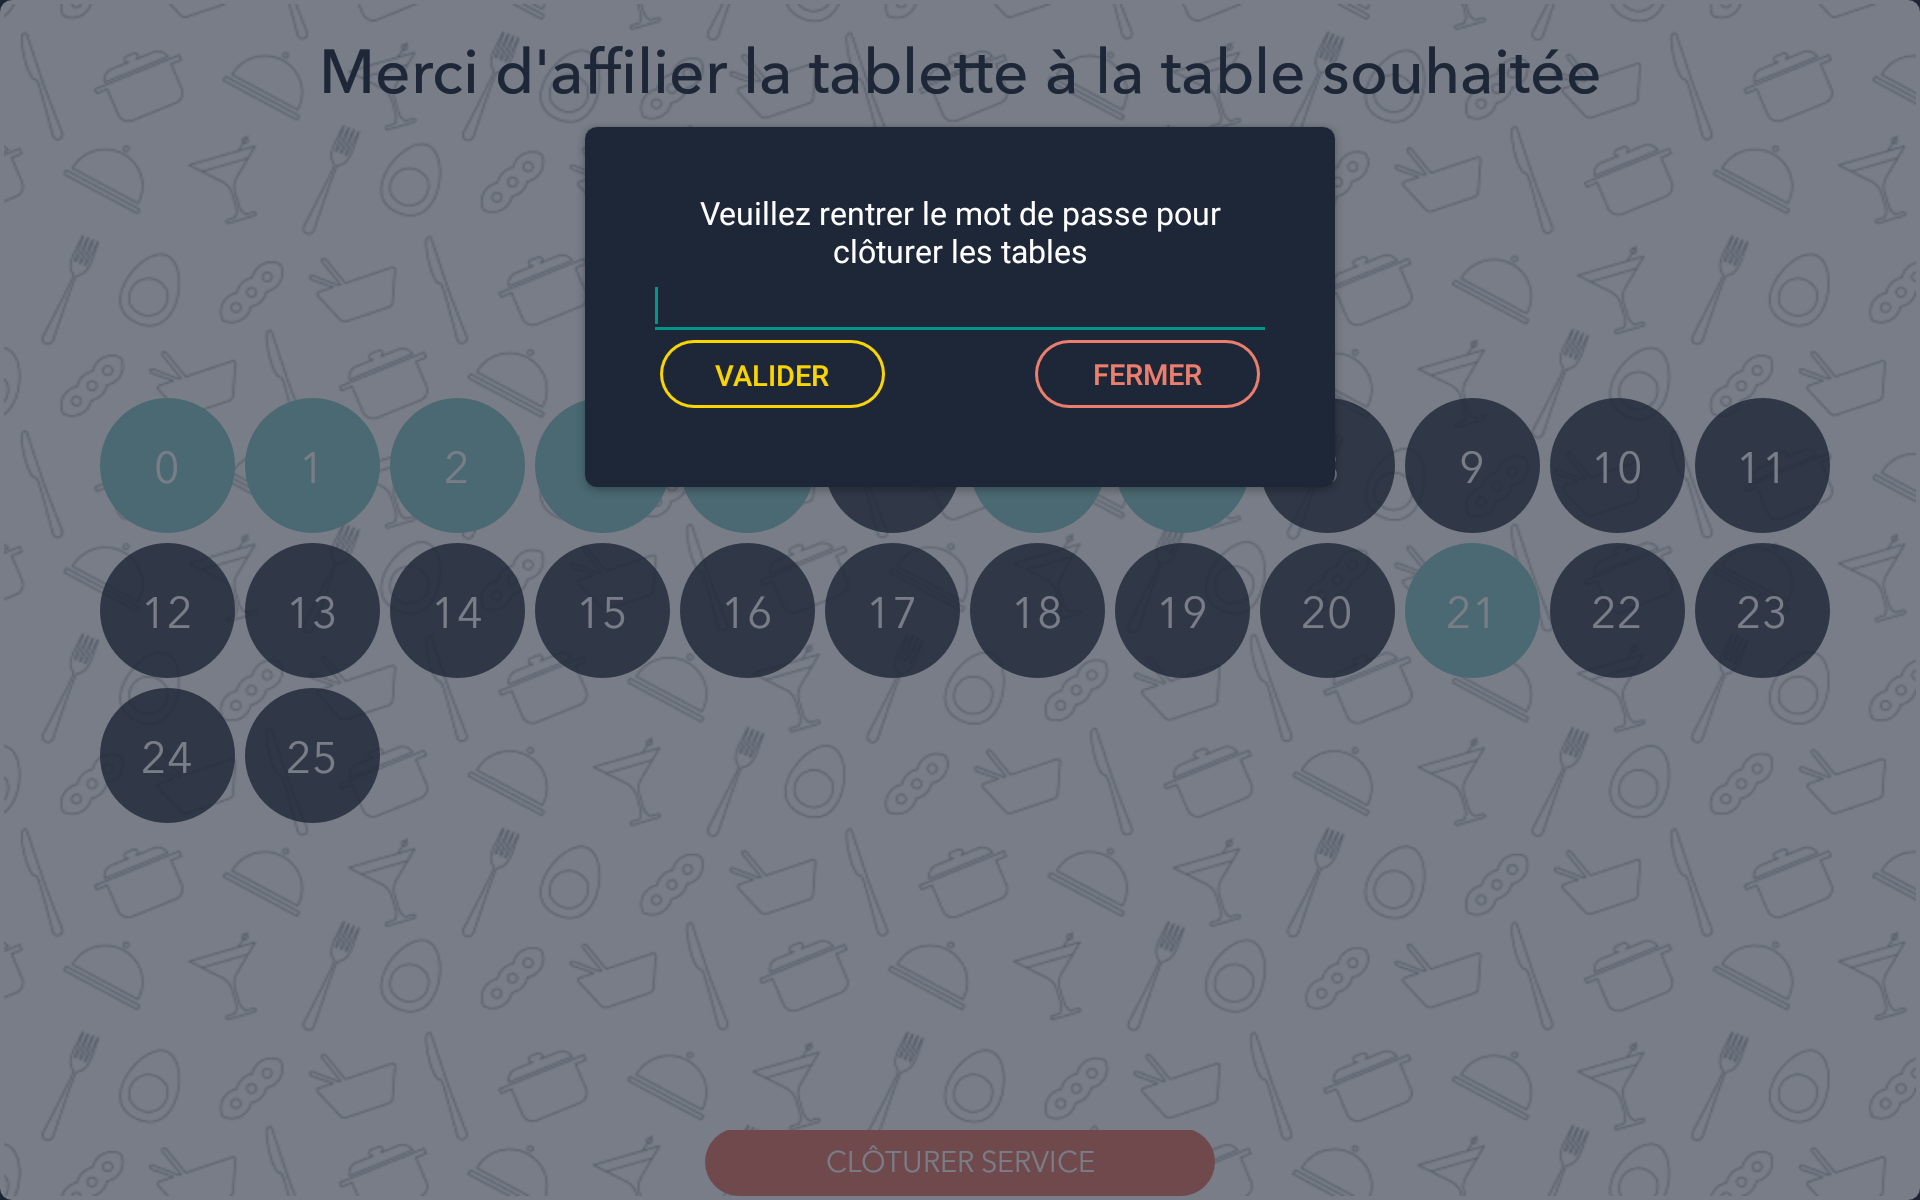
\includegraphics[width=100mm,scale=0.5]{images/cloture_table.png}
  \caption{Fenêtre pour la fermeture des tables}
  \label{fig:boat1}
\end{figure}

Le mot de passe demandé est toujours le même.Nous avons alors respecté la charte graphique qui existait déjà sur certaines autres pop-ups. Le but de cette mission était de sécuriser l'application pour la clôture de table. Fermer toutes les tables alors que l'on est en plein service peut s'avérer très dangereux.

\begin{figure}[!htb]
  \centering
  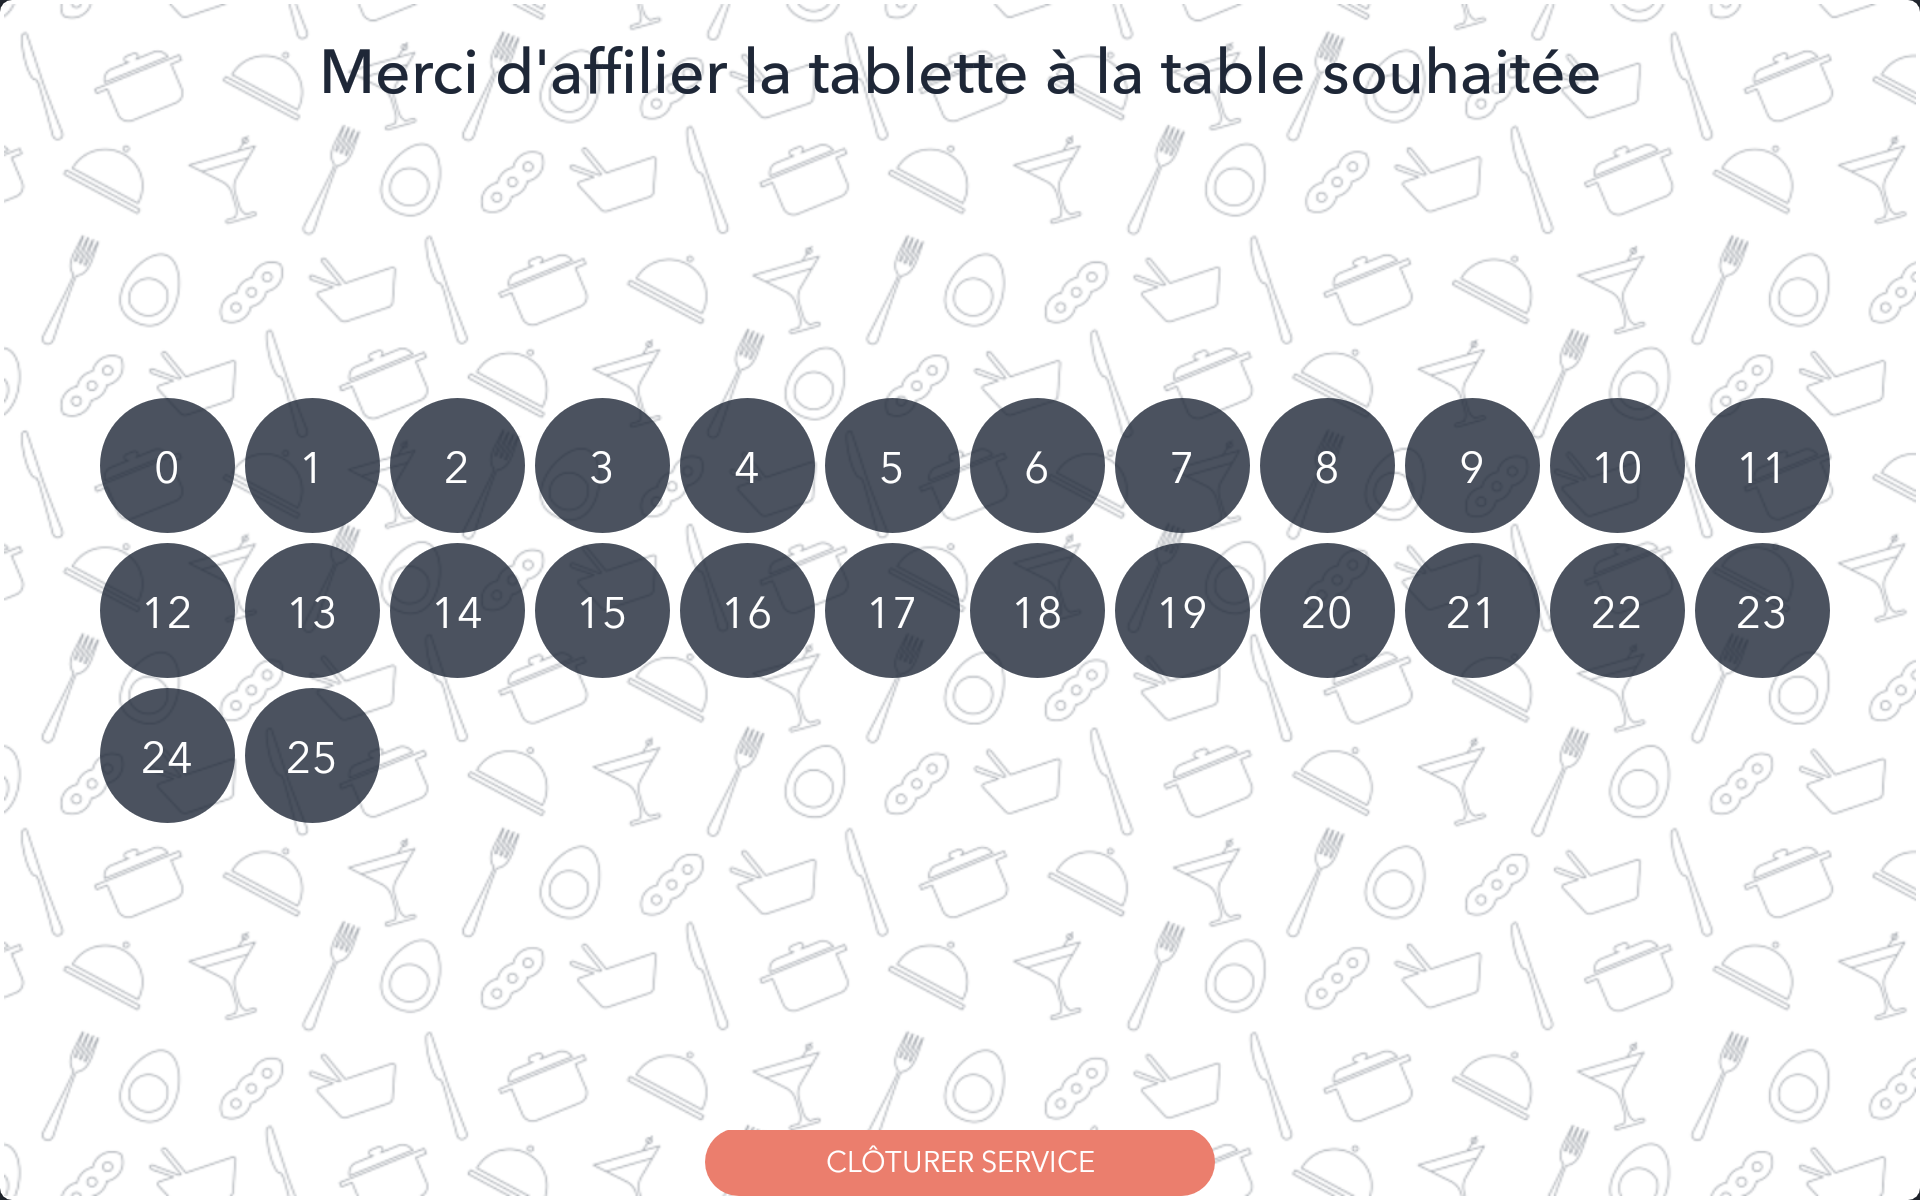
\includegraphics[width=100mm,scale=0.5]{images/cloture_table2.png}
  \caption{Toutes les tables sont fermés !}
  \label{fig:boat1}
\end{figure}


\subsection{Les descriptions scrollable visibles}

Certains produits possèdent des descriptions longues et dans certains cas l'aménagement du texte fait que l'on n'a pas forcément l'information que l'on peut scroller (ou dérouler) pour voir la suite.

\begin{figure}[!htb]
  \centering
  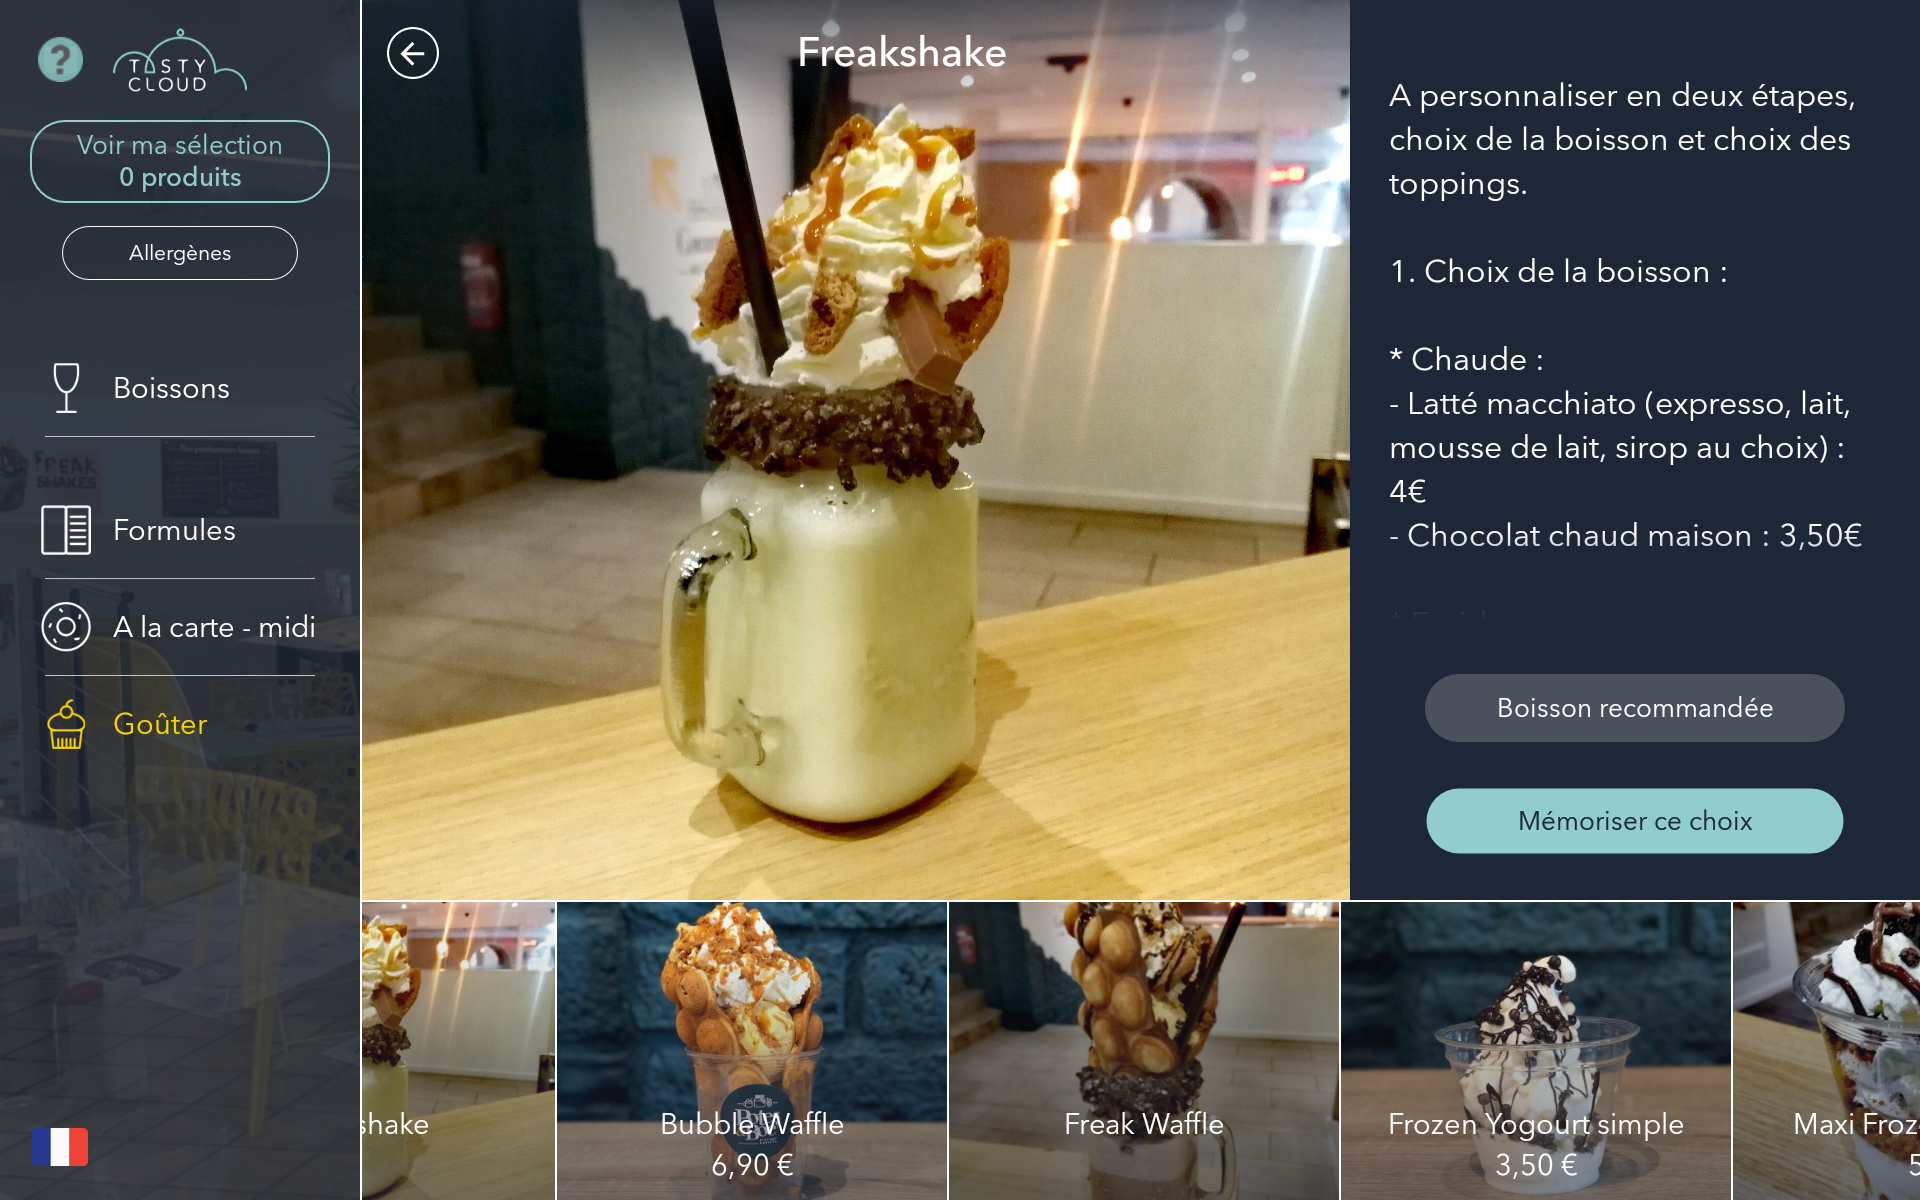
\includegraphics[width=100mm,scale=0.5]{images/scroll.png}
  \caption{Il est ici pas évident de savoir si on peut scroller}
  \label{fig:boat1}
\end{figure}

Voici par exemple un cas où le bas de la description coïncide avec un saut à la ligne. Ici le client peut passer à côté de ce qu'il y a écrit en dessous. Pour ce cas précis il s'agit d'expliquer une formule. Par conséquent il m'a été chargé de trouver un moyen pour régler ce problème. Ma première approche a été de changer la taille de la décoloration des bords pour que l'on voit mieux qu'il est possible de scroller vers le bas. Seulement, l'attribut à changer en XML fait que cela change le bas et le haut. J'ai alors fait en sorte que le bas du rectangle de description coïncide toujours avec une ligne de texte pour que cette dernière soit coupée. Ici le problème est que ce rectangle peut changer de taille. En effet pour les vins par exemple nous avons la provenance la date, ses caractéristiques qui prennent le haut droit de la page (au-dessus de la description). Par conséquent il est assez difficile de prévoir tous les cas possibles. 

J'ai donc abandonné cette idée pour finalement me rabattre sur la première mais cette fois en essayant de trouver une solution pour changer la décoloration juste en bas. En m'intéressant à la classe "ScrollView" d'Android (donc la classe qui nous permet de scroller), je me suis rendu compte que cette classe contenait deux fonctions "getTopFadingEdgeStrength" et "getBottomFadingEdgeStrength". Si le haut ne pose pas de problème il faut accentuer l'effet de décoloration du scrollview en bas. J'ai décidé de laisser le fonctionnement du "getBottomFadingEdgeStrength" comme il était mais de changer le top. Je voulais en effet limiter cette accentuation sur le top. Ainsi je pourrais utiliser l'attribut "FadingEgeLength" dans le XML en le mettant à un pourcentage élevé. Le top lui sera affecté à 20 pourcent de cette valeur avec la redéfinition de la fonction.

L'idée était donc de créer une classe qui étend de ScrollView et de redéfinir son "getTopFadingEdgeStrength" pour que ce dernier retourne 20 pourcents de la valeur qu'on lui a attribué dans le XML (le code de cette fonction est disponible en annexe). On utilisera alors cette classe comme ScrollView dans le XML.

\clearpage

\begin{figure}[!htb]
  \centering
  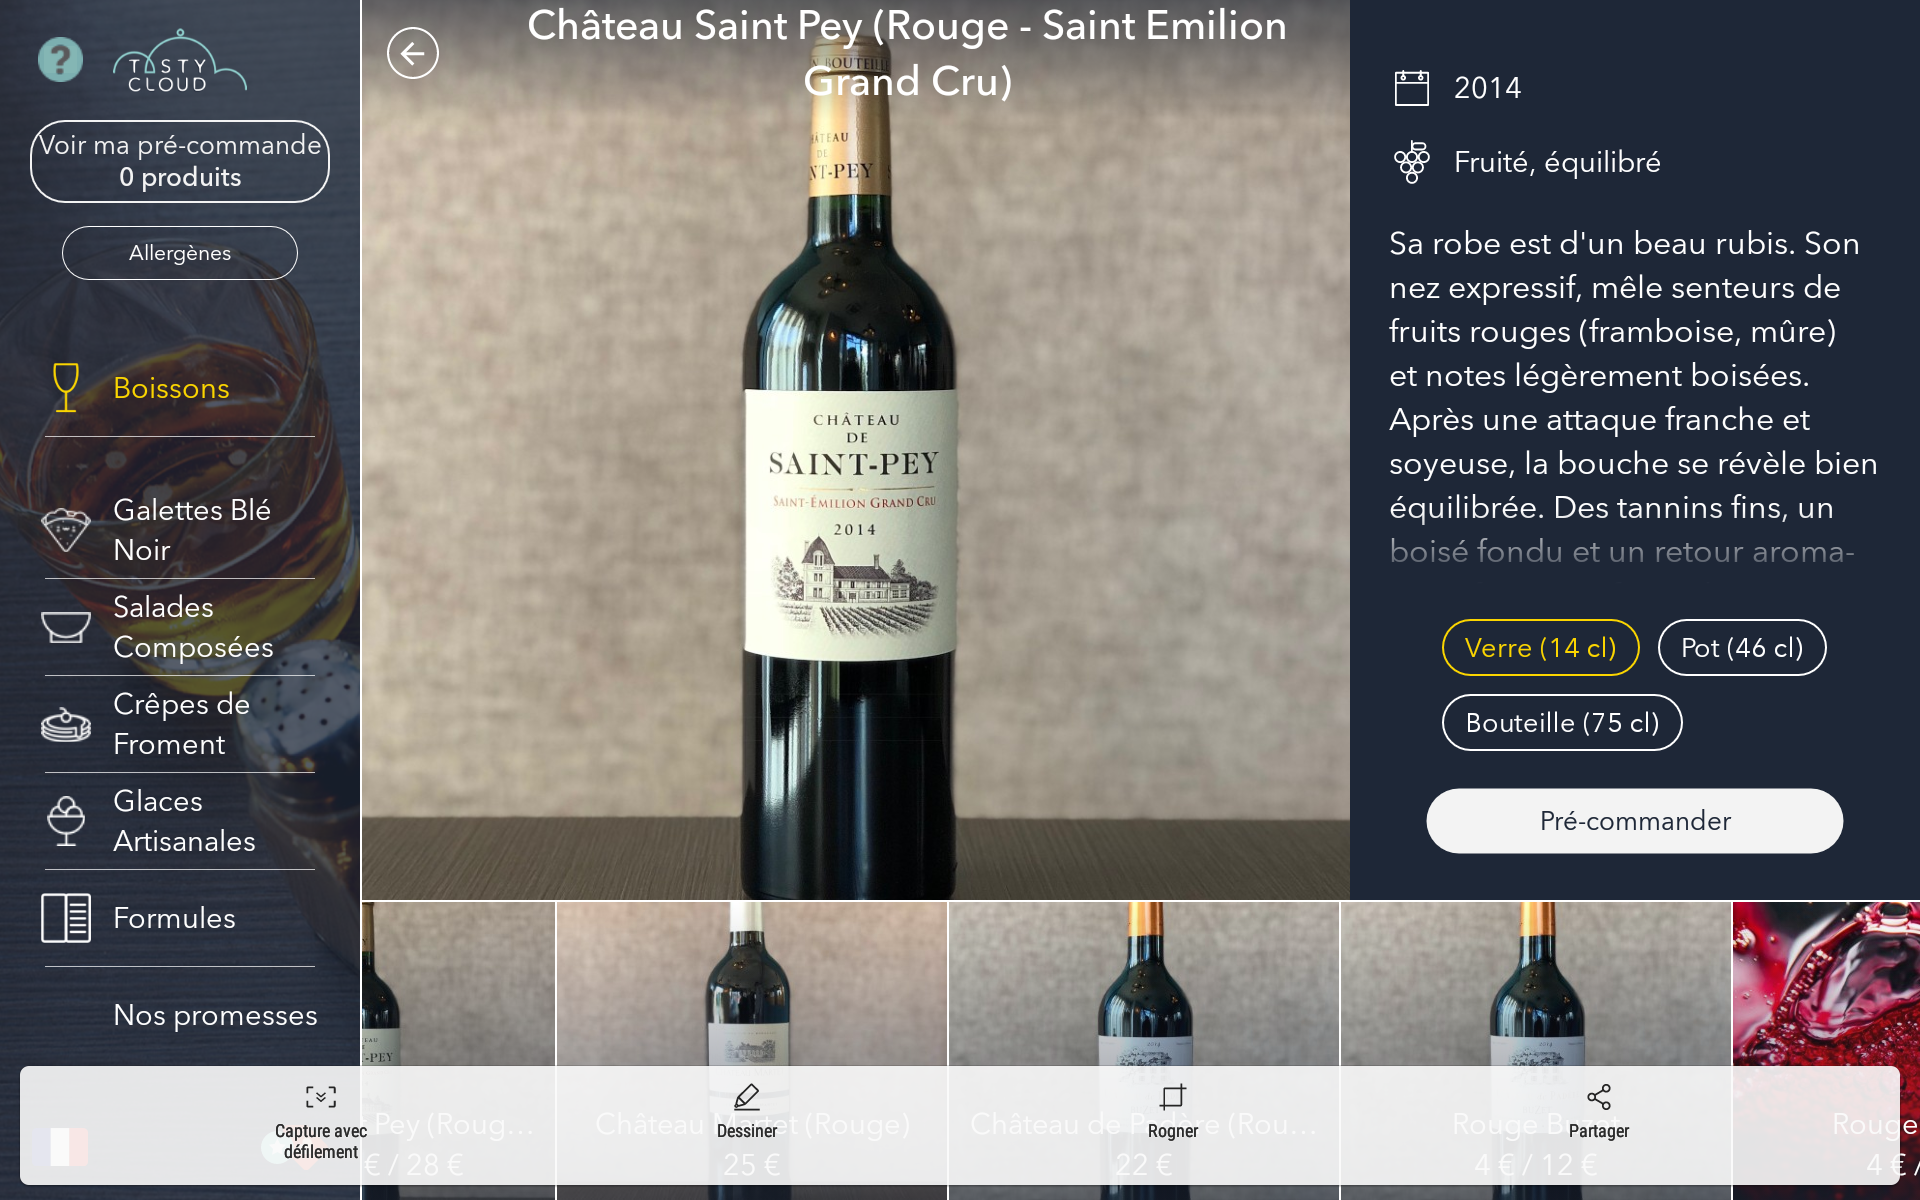
\includegraphics[width=115mm,scale=0.5]{images/scroll2.png}
  \caption{Effet de décoloration sur la description}
  \label{fig:boat1}
\end{figure}

On peut voir un exemple de cette décoloration sur la figure ci-dessus. J'en profite aussi pour montrer les caractéristiques présentes sur les vins par rapport à ce qui a été dit précédemment. On a par exemple ici la date et les caractéristiques du vin qui compressent la description. Pour la deuxième solution il était difficile de la mettre en place car il y avait trop de cas différents.

Par rapport à la décoloration, on voit bien ici que la description est scrollable. Prenons un autre cas où l'on voit bien la différence de taille entre le bas et le haut.

\begin{figure}[!htb]
  \centering
  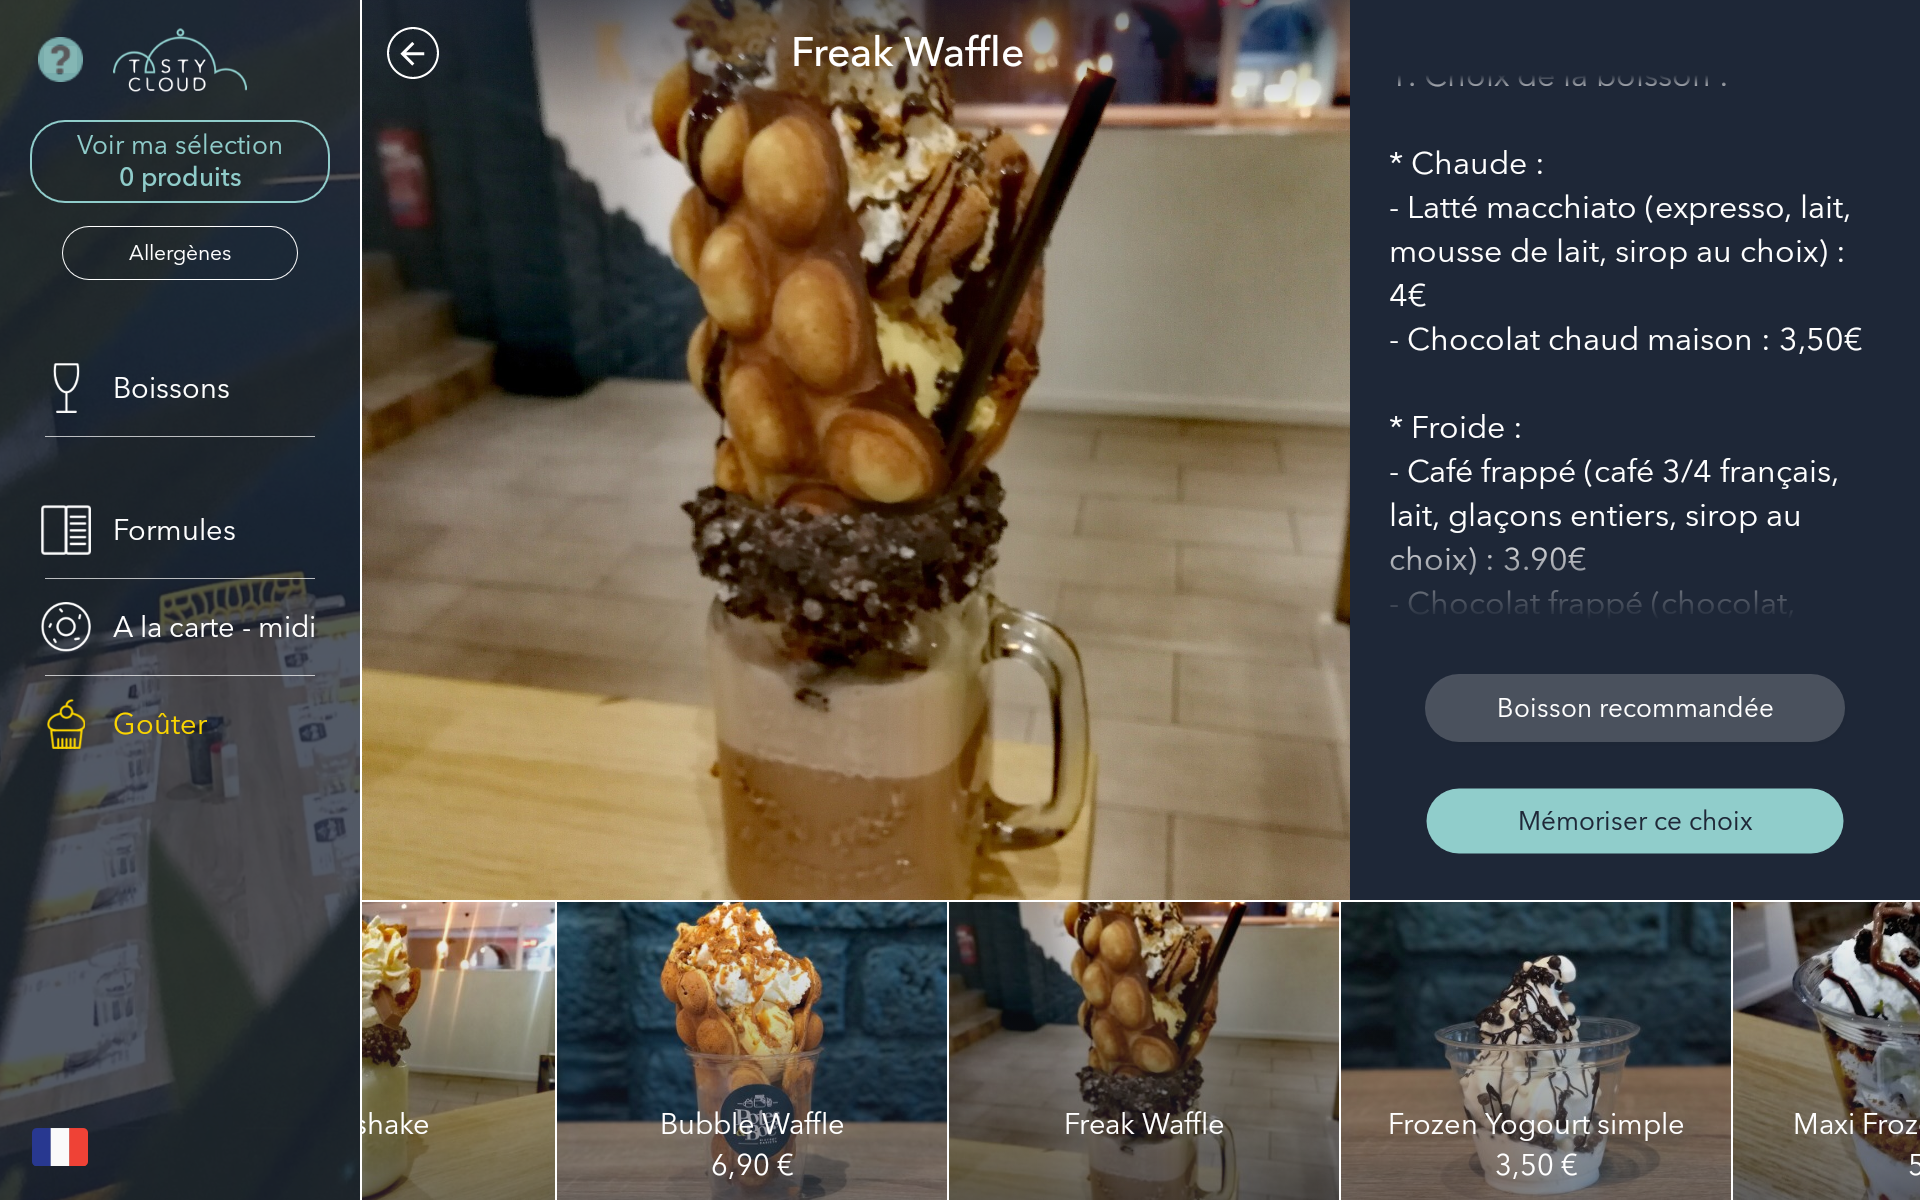
\includegraphics[width=115mm,scale=0.5]{images/scroll3.png}
  \caption{Différence décoloration haut et bas}
  \label{fig:boat1}
\end{figure}

Si dorénavant le bas de la description coïncide avec un retour à la ligne ou même un saut de ligne, l'utilisateur pourra constater le dégradé qui lui suggérera alors de dérouler la description. Cette mission peut paraître anodine mais elle tout de même importante pour accentuer la stabilité de l'application et montrer qu'il y a eu un gros travail sur le feedback client pour proposer la meilleure expérience possible aux utilisateurs.

\section{Divers}

Dans cette partie, je vais présenter différentes missions réalisées durant le stage qui sont soit minimes soit comparables à d'autres missions déjà présentées. Je vais aussi parler de choses pas directement en rapport avec ma mission de stage (donc le développement android).

Comme pour la mission du bouton blanc, une autre demande client était de cacher le total dans le menu de sélection où l'on voit ses plats choisis. Comme seulement quelques restaurants en particulier voulaient cette fonctionnalité, on a fait une option dans le back office. Il a donc juste fallu cacher le total dans le cas où la case correspondante à cette option était cochée. Voici un exemple où le total est caché, il n'est plus affiché en dessous de la liste des produits.

\begin{figure}[!htb]
  \centering
  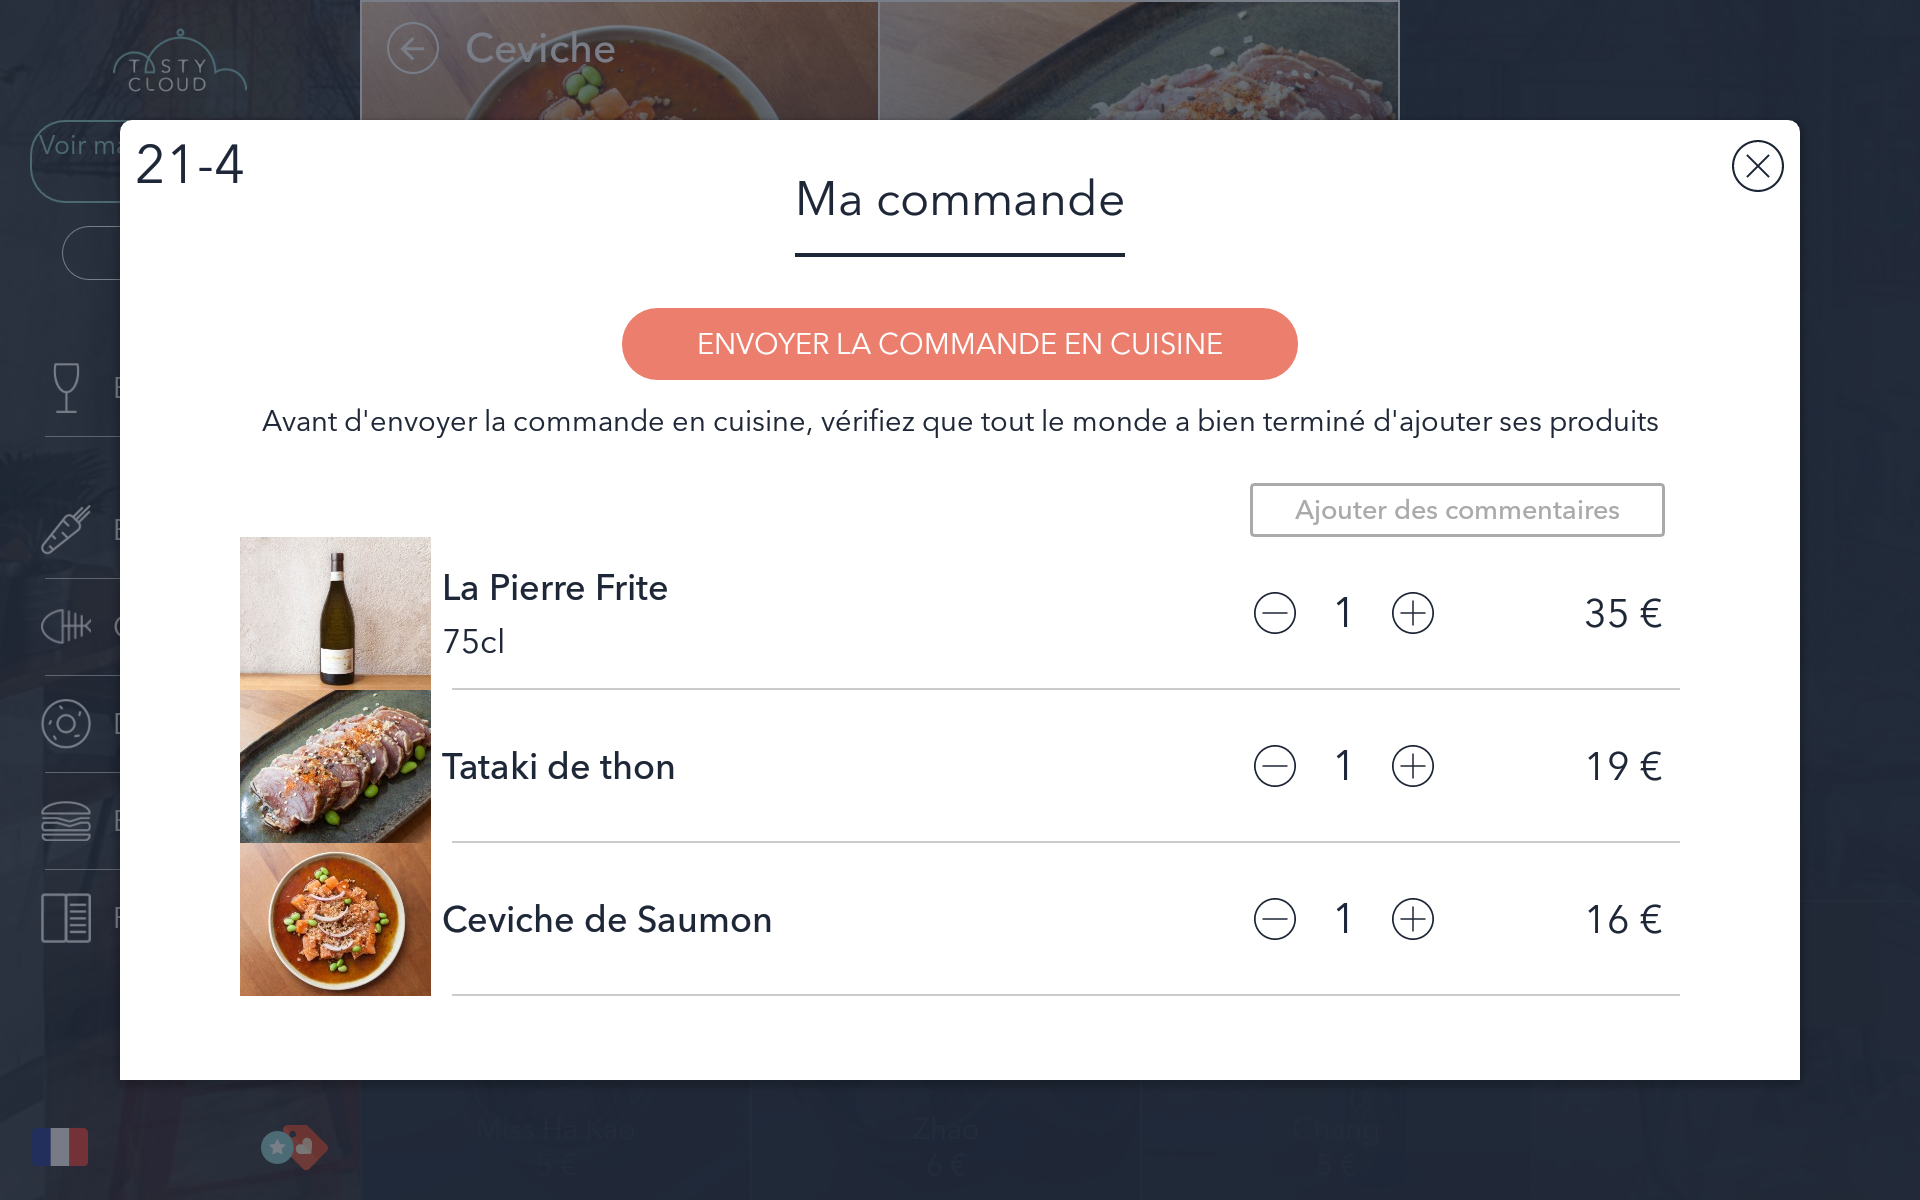
\includegraphics[width=115mm,scale=0.5]{images/divers.png}
  \caption{Le total est caché}
  \label{fig:boat1}
\end{figure}

Dans le menu d'accueil, le restaurateur peut mettre un message de bienvenue pour les clients avec des informations concernant le restaurant. Une demande a été de retirer ces messages (ça et le bouton à propos). Au lieu, cette fois, de mettre une option dans le back office, il a été décidé que dans le cas où le restaurateur décide de ne rien mettre en description et rien dans le bouton à propos, ces derniers ne s'affichent pas. Il a en effet la possibilité d'éditer ces informations dans le back office.

\begin{figure}[!htb]
  \centering
  \begin{minipage}[b]{0.45\textwidth}
    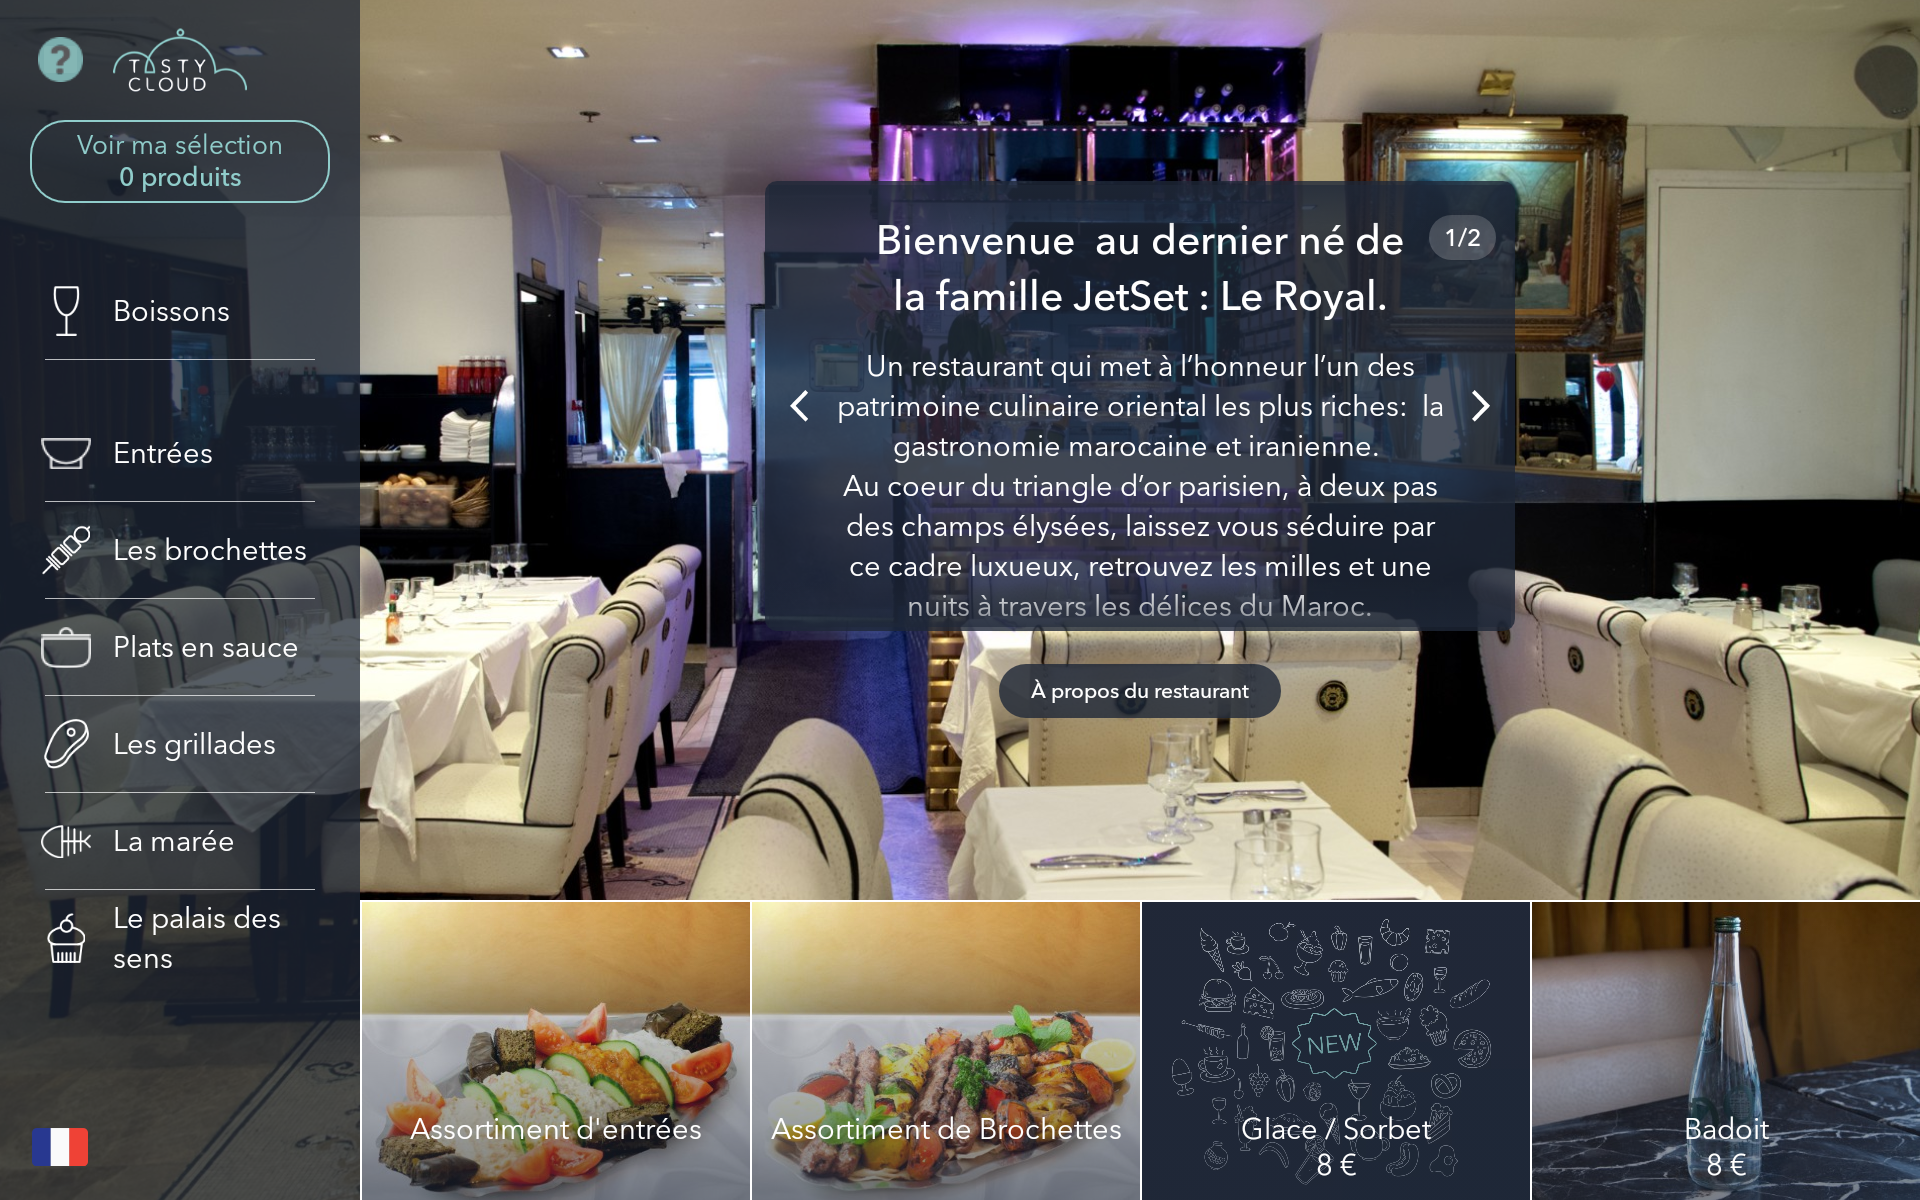
\includegraphics[width=\textwidth]{images/divers2.png}
    \caption{Informations sur l'accueil}
  \end{minipage}
  \hfill
  \begin{minipage}[b]{0.45\textwidth}
    \includegraphics[width=\textwidth]{images/divers3.png}
    \caption{Les informations sont cachées}
  \end{minipage}
\end{figure}

\clearpage

J'ai aussi réglé de nombreux petits bugs qui ont été remontés par des clients ou visibles lors de l'utilisation. Des bugs graphique, en rapport avec la base de données dont même certains qui faisaient crasher l'application. J'ai par exemple géré un cas ou des crashs arrivaient de façon irrégulière sur le changement de restaurant. J'ai fini par trouver le problème en débogage. J'ai refait tout le chemin de changement de restaurant en débogage jusqu'à trouver la cause du crash et pouvoir la régler. Dans ce cas le problème venait d'objets qui n'étaient pas chargés à cause du fait que l'application est asynchrone.

Pour d'autres bugs comme graphique j'ai réglé des détails dans les XML. Ces réglages peuvent être comparables à ce qui par exemple été fait sur le RecyclerView de l'affiliation. Il y a aussi eu des bugs dans le code qui ont engendré des bugs graphique. Par exemple j'ai travaillé sur un cas ou une mauvaise concaténation d'une chaîne de caractères entraînait une répétition du titre. J'ai aussi réglé un cas ou des mauvaises informations apparaissaient dans la sélection avec un chemin d'utilisation bien précis. J'ai aussi travaillé sur des mises à jour rapides. Par exemple sur le fait que les caractéristiques des vins (donc années caractéristiques etc ...) s'affichent si et seulement si nous avons une valeur. Avant l'icône restait même si il n'y avait pas d'informations.

J'ai décidé de ne pas faire de parties pour ces cas car il s'agissait de mises à jour relativement rapides. Par rapport au stage en lui-même, j'ai aussi aidé à la mise à jour sur le site web. Mon travail la dessus se limitait à du HTML et du PHP. J'ai mis à jour des redirections, textes, des pages. Par exemple, j'ai mis à jour certains clients et leur page web sur le site, j'ai fait de même pour la page qui énumère les articles parlant de l'entreprise. Je n'ai pas mis le site directement à jour mais j'ai tout envoyé sur bitbucket et mon tuteur s'est occupé du reste.

\begin{figure}[!htb]
  \centering
  \includegraphics[width=150mm,scale=0.6]{images/site_web_clients.png}
  \caption{Clients ajoutés (du Nokken au Mercure)}
  \label{fig:boat1}
\end{figure}

En plus du travail informatique, j'ai aussi aidé au développement de l'entreprise lorsque l'on mettait en place de nouveaux restaurants. Par exemple l'entreprise a eu un nouveau client avec 50 tablettes en mai et j'ai, avec une collègue, mis toutes les tablettes à jour sur le restaurant. Elles ont ensuite pu être envoyées chez le client. J'ai également mis à jour les photos sur 15 tablettes pour un autre restaurant. Bien que ces travaux n'étaient pas informatiques, ils ont en général toujours été en lien avec les tablettes.


\chapter{Synthèse}
\label{sec:synthese}
\section{Les résultats et améliorations possibles}

Mon stage a été l'occasion de réaliser de nombreuses missions. Ces dernières étaient plus ou moins importantes mais toutes ont été l'occasion d'apprendre de nouvelles choses et de mieux comprendre comment fonctionne l'application. Les missions les plus importantes restent le didacticiel ainsi que la remise en place de l'affiliation. En effet le nouveau système d'affiliation est aujourd'hui en place dans tous les restaurants qui possèdent cette option. Le premier restaurant que j'ai brièvement énoncé lorsque je parlais des 50 tablettes a été le premier à mettre ce nouveau système d'affiliation en place et jusqu'à ce jour nous n'avons pas connu de problème. 

L'autre mission importante du stage est le tutoriel. C'est la mission qui m'a demandé le plus de temps car il a fallu tout inventer, que ce soit la structure, le côté graphique avec le XML, la logique entre les étapes etc. C'est aussi pour cela que cette mission à été très intéressante. Cependant ce qui a été développé jusque-là n'est qu'une première version. Par conséquent il est fort possible que le tutoriel soit amélioré. D'ailleurs, à ce stade de développement on peut déjà penser à des améliorations côté visuel comme côté code. Celle qui me vient le plus à l'esprit concerne l'éclaircissement des éléments. Techniquement on utilise des coordonnées en "dur" pour les rectangles éclaircis. C'est d'ailleurs quelque chose qui a pris du temps de développement. J'ai du étalonner en faisant plusieurs essais avec différentes valeurs. Pour certaines vues les coordonnées sont récupérées. Pour d'autre les vues sont dans d'autres layouts et il est plus difficile de les obtenir car ce ne sont pas des vues d'Android mais de l'application propre et les récupérer enclenchait des bugs. C'est d'ailleurs pour cela qu'il y a des redéfinitions de fonctions dans les fonctions de type "setBrightView". Il y a des cas où l'on a un seul paramètre et c'est la vue et d'autre ou on a les coordonnées. Une autre amélioration possible est de donner plus de "pouvoir" à l'utilisateur (ici comprendre le restaurateur). Il pourrait par exemple dans le futur avoir la possibilité de gérer lui-même ses étapes de tutoriel, choisir ses couleurs de pop-up etc. Il a aujourd'hui seulement la possibilité de changer les textes.

Pour toutes les missions énoncées, ces dernières ont été mises en production et le résultat est qu'aujourd'hui l'utilisateur à accès à ces nouvelles fonctionnalités. Comme expliqué précédemment certaines sont optionnelles (affiliation, didacticiel). L'avantage pour les clients est que les nouvelles fonctionnalités sont intégrées à l'offre Tastycloud. Par conséquent ce sont des sortes de promesses que fait l'entreprise et le client reçoit ces ajouts. Bien évidemment, ces fonctionnalités sont souvent en rapport avec des demandes clients ou du feedback mais d'autres clients pouvaient n'avoir rien demandé et c'est une réelle plus-value pour le client qui est alors témoin du sérieux et de l'efficacité de la solution.

\section{Ce que j'ai appris}

Ce travail chez Tastycloud m'a appris des notions de développement plus poussé que lors de mes précédents stages. J'ai, en effet ici appris à mettre en oeuvre un schéma d'utilisation et à conceptualiser et modéliser un système informatique. Cela a été très enrichissant et stimulant d'un point de vue ingénierie car on a le sentiment d'avoir avancé en compétence par rapport à ce qu'on a pu faire par le passé. D'un point de vue plus technique j'ai appris un nouveau langage kotlin et de nouveaux principes Android. J'ai appris des choses côté graphique avec le XML. C'est un stage qui demande beaucoup d'autonomie dans les recherches c'est aussi pourquoi j'ai appris à bien cibler mes recherches pour trouver des solutions efficaces rapidement. 

Comme c'était la première fois que j'étais confronté à un cas concret d'application Android j'ai aussi été sensibilisé au fonctionnement d'une application dans le monde de l'entreprise. Cela a été intéressant de voir comment marchait l'évolution de la maintenance de ce genre d'application. D'un point de vue moins technique j'ai aussi été confronté au travail en start-up et également en openspace qui est aussi une expérience formatrice.

    
\chapter{Conclusion}
\label{sec:conclusion}

En conclusion, ce stage chez Tastycloud à été une expérience enrichissante, formatrice, intéressante et même conviviale ! J’ai été amené tout au long du stage à faire preuve d’autonomie dans la recherche d’informations et également à découvrir un tout nouveau milieu : celui de la start-up. J'ai aussi été sensibilisé au monde de la restauration pour bien comprendre les spécificités de l'application. Chaque restaurant a ses propres caractéristiques et son propre vocabulaire, ses propres besoins auxquels il faut s'adapter. J'ai donc appris toutes ces choses au fur et à mesure et avec l’aide principalement de mon tuteur et au reste de l'équipe.

J'ai développé des compétences techniques que ce soit en Kotlin ou Android. Bien que j'ai été dans un premier temps un peu perdu surtout en commençant par la mission de l'affiliation. J'ai réussi à me former en apprenant par moi-même et avec l'aide de mon tuteur. Les sites web tels que "stackoverflow" m'ont aussi bien aidé pour comprendre certains détails techniques que ce soit encore une fois en Android ou en Kotlin. J'ai dorénavant bien conscience de la manière dont fonctionne l'application et tous les enjeux autours. Je pourrai, je pense, réutiliser toutes ses connaissances dans le futur surtout que je souhaite m'orienter dans le développement mobile. Enfin, ce stage a été un bon exemple de pourquoi il faut documenter son code, pourquoi il est important de poser des schémas et des diagrammes UML avant de commencer le développement d'un projet la réflexion étant mise en avant tout le long du projet. Cette réflexion se fait d'un point de vue utilisateur (comment va-t-il utiliser cette fonctionnalité ?) ou d'un point de vue réutilisation du code, ce qui a été énoncé durant le rapport.

Cette partie du stage s'est donc bien déroulée. Cependant ce dernier se termine en août et par conséquent j'ai de nouvelles missions qui m'attendent cet été. Notamment une mission de customisation des produits (par exemple choisir les ingrédients de sa pizza). Je suis ainsi fier de participer aux enjeux de l’entreprise à travers les missions qui m’ont été confiées. Le projet de Tastycloud étant innovant et original il m'a été facile de me motiver pour y travailler surtout qu'on m'a donné une certaine liberté dans le développement. Savoir que certaines des fonctionnalités que j'ai développées peuvent être utilisées par des milliers de clients est une immense satisfaction. C'est pour tout cela que Tastycloud est pour moi une expérience élémentaire de mon parcours universitaire.

\begin{figure}[!htp]
  \centering
  \includegraphics[width=130mm,scale=0.5]{images/equipe.jpg}
  \caption{Photo de l'équipe}
  \label{fig:boat1}
\end{figure}

\chapter{Annexe}
\label{sec:annexe}

\underline{Fonctionnement du système presenter, controller, adapter ... :}

\begin{figure}[!htp]
  \centering
  \includegraphics[width=130mm,scale=0.5]{images/diagramme_conttroller.png}
  \caption{Fonctionnement du système "controller"}
  \label{fig:boat1}
\end{figure}

Ce système marche avec Dagger. Repository est la classe qui fait lien avec la base de données et Home appelle les controller.

\underline{Texte du didacticiel :}

1) Bonjour et bienvenue chez X ! Nous allons vous montrer comment passer commande depuis cette tablette.
Cela ne vous prendra que quelques secondes.
Non, merci / Continuer

2) Retrouvez ici les suggestion de l'établissement.
Suite

3) Allergique ou intolérant ? Sélectionnez ici les éléments qui vous concernent, une icône apparaitra alors sur les produits qui en contiennent.
Suite

3) Naviguez entre les différentes catégories pour faire votre choix.
Suite

4) Cliquez sur un produit pour en voir tous les détails.
Suite

5) Vous désirez autre chose ? Appuyez sur la flèche pour revenir à l'écran précédent
Suite

6) Celui-ci vous plait et vous souhaitez le commandez ? Cliquez sur "mémoriser" ou sur "personnaliser et mémoriser" s'il y a des options à choisir pour l'ajouter à votre sélection.
Suite

7) Une fois votre choix fait, retrouvez les plats que vous avez retenus dans l'onglet "sélection".
Suite

8) Votre sélection vous convient et vous êtes prêts à commander ? Cliquez sur "envoyer ma commande en cuisine", un serveur viendra vous apporter votre premier plat dès que le chef l'aura préparé.
Suite

9) Si malgré tout vous avez des doutes, n'hésitez pas à appeler un serveur qui viendra vous aider avec grand plaisir. Bon appétit !
Fin

\clearpage
\underline{Capture d'écran didacticiel :}

\begin{figure}[!htb]
  \centering
  \begin{minipage}[b]{0.45\textwidth}
    \includegraphics[width=\textwidth]{images/tuto7.png}
    \caption{Message bienvenue}
  \end{minipage}
  \hfill
  \begin{minipage}[b]{0.45\textwidth}
    \includegraphics[width=\textwidth]{images/tuto2.png}
    \caption{Étape 1}
  \end{minipage}
\end{figure}

\begin{figure}[!htb]
  \centering
  \begin{minipage}[b]{0.45\textwidth}
    \includegraphics[width=\textwidth]{images/tuto3.png}
    \caption{Étape 2}
  \end{minipage}
  \hfill
  \begin{minipage}[b]{0.45\textwidth}
    \includegraphics[width=\textwidth]{images/tuto4.png}
    \caption{Étape 4}
  \end{minipage}
\end{figure}

\begin{figure}[!htb]
  \centering
  \begin{minipage}[b]{0.45\textwidth}
    \includegraphics[width=\textwidth]{images/tuto5.png}
    \caption{Étape 6}
  \end{minipage}
  \hfill
  \begin{minipage}[b]{0.45\textwidth}
    \includegraphics[width=\textwidth]{images/tuto6.png}
    \caption{Étape 9}
  \end{minipage}
\end{figure}

\clearpage

\underline{Code du TouchDelegate}

\begin{lstlisting}[frame=single]  % Start your code-block
    
        fun setExtraRectangleClickable (minView: View, extraTop: Int, 
        extraLeft: Int, extraBottom: Int, extraRight: Int) {

        //initialisation du pere de la vue
        var bigView = minView.parent as View

        bigView.post({
            //recuperation du rectangle entourant la vue
            var rect = Rect()
            minView.getHitRect(rect)

            //ajout des dimensions elargies
            rect.top -= extraTop.dp
            rect.left -= extraLeft.dp
            rect.bottom += extraBottom.dp
            rect.right += extraRight.dp

            //creation du touch delegate
            var touchDelegate = TouchDelegate(rect, minView)
            this.addDelegate(touchDelegate)

            //affectation du delegate au pere
            bigView.touchDelegate = this

        })

    }
    
\end{lstlisting}

\underline{Code du ScrollView :}

\begin{lstlisting}[frame=single]  % Start your code-block
    
   override fun getTopFadingEdgeStrength(): Float {
        if (childCount == 0) {
            return 0.0f
        }

        val length = verticalFadingEdgeLength
        if (scrollY < length) {
            if((scrollY / length.toFloat()) >= 0.2f)
                return 0.2f
            else
                return scrollY / length.toFloat()
        }

        return 0.2f

    }

\end{lstlisting}

On force à toujours retourner 0.2f après un cap

\clearpage
\underline{Page web changées :}

http://www.tastycloud.fr/clients-menu-sur-tablette-tactile.html

http://www.tastycloud.fr/press-restaurant-connecte-digital.html

\chapter{Bibliographie}
\label{sec:bibliographie}

Site web de Tastycloud : 

http://www.tastycloud.fr

Recherche web principalement sur : 

https://stackoverflow.com/

https://developer.android.com/

Aide Kotlin : 

http://tutos-android-france.com/introduction-a-kotlin/




%%% Local Variables: 
%%% mode: latex
%%% TeX-master: "isae-report-template"
%%% End: 








\appendix

\end{document}